\documentclass[12pt]{report}
\usepackage[utf8]{inputenc}
\usepackage[style=apa,sortcites=true,sorting=nyt,backend=biber]{biblatex}
\addbibresource{EBC.bib}
\usepackage[
            colorlinks=true,        
            allcolors = black,  
            citecolor=blue,        
        ]{hyperref}
\AtEveryCite{\color{blue}}       

\usepackage{graphicx}
\graphicspath{ {images/} }
\usepackage{graphicx} % Required for inserting images
\usepackage[titles]{tocloft}
\usepackage{sectsty}
\usepackage{amsmath}
\usepackage{mathtools}
\usepackage{amssymb}
\usepackage{stmaryrd}
\usepackage{comment}
\usepackage{dsfont}
\usepackage{algorithm}
\usepackage{algpseudocode}
\usepackage{caption}
\linespread{1.5}




\def\cred{\color{red}}
\def\cblue{\color{blue}}
\newtheorem{remark}{Remark}[section]
\newtheorem{exam}{\textsc{Example}}[section]
\newtheorem{theorem}{Theorem}[subsection]
\newtheorem{proposition}{Proposition}[section]
\newtheorem{lemma}{Lemma}[subsection]
\newtheorem{algorithmold}{Algorithm}[section]
\newtheorem{definition}{Definition}[subsection]
\newcommand{\1}{\mathbf{1}}
%\newcommand{\1}{\mathds{1}}
\def\be{\begin{equation}}
\def\ee{\end{equation}}

\usepackage[a4paper, portrait, margin=0.9in]{geometry}

\sectionfont{\LARGE}
\subsectionfont{\Large}
\subsubsectionfont{\large}

\setcounter{tocdepth}{4}
\setcounter{secnumdepth}{4}

\begin{document}

\begin{titlepage}
   \begin{center}
       \vspace*{1cm}
        \huge
       \textbf{Class of Empirical Copulas:} \\
       \huge
       \textbf{Modelling Tail Risk} \\
       \vspace{2cm}
        \LARGE
       \textbf{Tong Pun Yat}

       
        
       \vspace{7.0cm}
       \Large
       STAT4798 Statistics and Actuarial Science Project
            
       \vspace{0.8cm}
            
       Department of Statistics and Actuarial Science\\
       The University of Hong Kong\\
       30 April 2024
            
   \end{center}

\end{titlepage}

\newpage
\begin{flushleft}
\LARGE
\textbf{Preface} \\
\normalsize
\vspace{1cm}
Prof. Hofert has provided inspiration and motivation behind this project (understanding the overestimation and underestimation of tail risk). I have developed the algorithm in its entirety, and is reviewed by Prof. Hofert, where he has given comments on how to improve the simulation. The report is also typed entirely by me, where the first half of the report are prerequisites, which are in reference with various relevant literatures (most notably \cite{HofertBook}, \cite{KojadinovicYi2024Smooth}, \cite{SegersEBC}); and the second half of the report is original, with parts of the R code referencing \cite{copulaRPackage2023}, \cite{KojadinovicYi2024Smooth} with some modifications from me. 
\end{flushleft}

\newpage
\begin{flushleft}
\LARGE
\textbf{Acknowledgements} \\
\normalsize
\vspace{1cm}
I would like to thank Prof. Hofert, my supervisor for STAT4798, for his continued guidance in the entirety of this project, where he has introduced the underlying motivation around this topic and on copulas overall. I would also like to especially thank my friend Yao Hui for assisting in running the (super long) R algorithm for me (as my computer did not have sufficient memory / RAM to handle the simulation). I would also like to thank my friends for their continued support during this course, and lastly my girlfriend Tiffannie, or I wouldn't have stood till now.
\end{flushleft}

\tableofcontents
\renewcommand\thesection{\arabic{section}}

\newpage
\begin{flushleft}
\sectionfont{\fontsize{20}{15}\selectfont}
\subsectionfont{\fontsize{17}{15}\selectfont}
\section{Introduction}
\vspace{0.5cm}
\subsection{Motivation}
\vspace{0.5cm}
\normalsize
In introductory statistics, we borne the need to understand the relationship between multiple underlying variables to make statistical inference. By analysing them in a univariate way, we gain intuition on the distributional characteristics of its marginal distribution, while multivariate analysis allow us to understand the dependence between variables. To begin with, we can start with linear dependence. Notably, we generalise the linear relationship between variables with correlation coefficients: \\
\vspace{0.5cm}
\begin{align*}
\rho = \begin{pmatrix} 
    1 & \rho_{12} & \dots & \rho_{1d} \\
    \rho_{21} & 1 & \dots & \rho_{2d} \\
    \vdots & \vdots & \ddots & \vdots \\
    \rho_{n1} & \rho_{n2} & \dots & 1
\end{pmatrix}
, \: \rho_{ij} = \frac{Cov(X_{i},X_{j})}{\sqrt{Var(X_{i})Var(X_{j})}}
\end{align*} \\
\vspace{0.5cm}
However, we realise that this metric is only useful when evaluating linear relationships between variables (or transformed variables). A low correlation coefficient does not imply a weak relationship as variables might exhibit non-linear dependence. \\
\vspace{0.5cm}
Copulas, as investigated in this report, can describe the dependence between the components of the random vectors. However in reality, while dealing with messy datasets, it is extremely hard to infer the unknown Copula and marginal distributions by observation. Parametric or semiparametric methods of estimating the copula are often biased as the parametric family of copulas have to be specified beforehand, which is often unrealistic. A possible workaround of this problem is utilising nonparametric estimation of copulas, which does not require prior knowledge on the family of copulas when undergoing statistical inference. \\
\vspace{0.5cm}
Empirical copula, first proposed by \cite{DeheuvelsEC}, analyses the multi-dimensional psuedo-observations (estimated nonparametrically as the ranks of the components of the random vector) componentwise, and could be shown to have a similar shape to the real estimated copula. However, empirical copula is shown to not be a copula itself due to its discrete uniformity on the marginal distribution of the random vectors. \\
\vspace{0.5cm}
To overcome this shortcoming, multiple smoothed copulas built on the basis of empirical copulas are proposed. It includes a multilinear extension of the empirical copula, the empirical checkerboard copula (as defined by \cite{CarleyTaylorECC} and \cite{HofertBook}), the empirical beta copula \parencite{SegersEBC}, and recently, generalised smooth copula estimators (that contains the empirical beta copula) proposed by \cite{KojadinovicYi2024Smooth}. \\
\vspace{0.5cm}
In present time, tail risk is widely less understood and often underestimated. It is known that the usage of the no-tail-dependent Gaussian Copula in the modelling of default probability of securities (and tranches) with mortgage underlyings have indirectly led to the financial crisis in 2007, where securities are mispriced due to the underestimation of tail default risk. The usage of the wordings "1-in-500" in describing the massive flood that happened in Hong Kong during late 2023 is widely misunderstood, as there are no 500-year worth of data in understanding an event of this scale. Yet, due to global warming, these large scale national disasters will be recurring (or even commonplace) in the near future, which brings the urgency in developing tail risk modelling techniques. \\
\vspace{0.5cm}
In this report, we try to understand whether the class of empirical copulas systematically underestimate or overestimate tail risk with respect to the true underlying copula by computing the up-tail and low-tail probability of the class of empirical copulas and compare it to the true up-tail and low-tail probability. This could extend the possibility that even for a small sample size empirical copula can be more widely applied in the modelling of tail risks without the risk of misspecifying the class of copulas and with added accuracy compared to other parametric / semiparametric methods. \\
\vspace{0.5cm}

\newpage

\section{Prerequisites: Copulas}
\vspace{0.5cm}
\subsection{Definition and Construction}
\vspace{0.5cm}

We first establish two important (and well-known) results on probability transformation. When $F$ is a continuous distribution, $F^{-1}$ is equivalent to the inverse of $F$.\\


\begin{lemma}\label{IntegralTransform} 
\textbf{Integral Transform} \\

For a r.v. $X$ $\sim$ $F$ where $F$ is a continuous distribution function $\Rightarrow$ $F(X)$ $\sim$ $U(0,1)$.
\end{lemma}
Proof:  \parencite{HofertBook} $F_{F_{X}}(x)$ = $P(F_{X}(x) $$\le$ $y$) = $P(X \le F^{-1}_{X}(y))$ = $F_{X}(F^{-1}_{X}(y))$ = $y \Rightarrow F(X)$ $\sim$ $U(0,1)$ 
\\


\begin{lemma}\label{QuantileTransform}
\textbf{Quantile Transform} \\

For a r.v. $U \sim U(0,1)$, $F$ and $F^{-1}$ being any distribution function and its corresponding quantile function respectively $\Rightarrow$ $F^{-1}_{X}(U) \sim F $.
\end{lemma}
Proof: Similar to \textbf{Lemma 1.1}, $P(F^{-1}_{X}(U) \le x) = P(U \le F_{X}(x)) = F_{X}(x)$
\\

\vspace{0.5cm}
These two transformation implies that it is trivial to transform any continuous distribution into a standard uniform distribution, and subsequently to another continuous distribution of interest. This allows us to relate random variables with different underlying distributions easily. We can generalise dependence by creating a continuous multivariate distribution function that links all the marginal standard uniform distributions. 

\vspace{0.5cm}
The definition of Copula is illustrated below, with reference to \cite{HofertBook}.\\

\begin{definition}\label{CopProperties}
\textbf{Copula} \\
A copula is a continuous d-dimensional distribution function $C(u_{1}, u_{2}, \dots, u_{d}) $ that satisfies the following properties: \\
\begin{enumerate}
    \item Groundedness: \: $C(u_{1}, \dots, u_{i-1}, 0, u_{i+1}, \dots, u_{d}) = 0$ if any $u_{i} = 0$.\\
    \item $U(0,1)$ margins: \: $\forall i \in \{1, \dots,d\}, \: C(1, \dots, 1, u_{i}, 1, \dots, 1) = u_{i}$\\
    \item d-increasing: $\: \textbf{a}, \textbf{b} \in [0,1]^{d}, \Delta_{(\textbf{a},\textbf{b}]}C = \sum\limits_{i \in \{0,1\}^{d}} (-1)^{\sum_{j=1}^{d}i_{j}}C(a_{1}^{i_{1}}b_{1}^{1-i_{1}}, \dots, a_{d}^{i_{d}}b_{d}^{1-i_{d}})  \ge 0 $, \: where $\Delta_{(\textbf{a},\textbf{b}]}C$ is the C-volume defined w.r.t hyperrectangle $(\textbf{a},\textbf{b}]$.
\end{enumerate}
\end{definition}


% cite sklar
What makes copulas so popular is its uniqueness under a continuous framework. This is brought about by the famous results of Sklar's Theorem.

\begin{theorem}\label{SklarTheorem}
\textit{\normalfont \parencite{SklarTheorem}}
\textbf{Sklar's Theorem}
\vspace{-0.2cm}
\begin{enumerate}
    \item Existence: For univariate margins $F_{1}, F_{2}, \dots, F_{d} \sim U(0,1)$, a d-dimensional distribution function $F$, $\exists C: [0,1]^{d} \rightarrow [0,1]$ such that $F(\textbf{x}) = C(F_{1}(x_{1}), \dots, F_{d}(x_{d}))$, $\textbf{x} \in \mathbb{R}^{d}$, where $C$ is uniquely defined on $\prod_{j=1}^{d} ran \: F_{j}$.
    \item Converse: Given any copula $C: [0,1]^{d} \rightarrow [0,1]$ and univariate margins $F_{1}, F_{2}, \dots, F_{d}$, $F(\textbf{x}) = C(F_{1}(x_{1}), \dots, F_{d}(x_{d}))$ is a d-dimensional distribution function, $\textbf{x} \in \mathbb{R}^{d}$.
\end{enumerate}
\end{theorem}
Notice that if the univariate margins $F_{1}, F_{2}, \dots, F_{d}$ are continuous (and $U(0,1)$ distributed), $C$ is uniquely defined. \\
\vspace{0.5cm}
This shows that there is a one-to-one correspondence between the univariate margins to the observable d-dimensional distribution function, linked by a unique copula function. \\
\vspace{0.5cm}

Its' significance can be illustrated by the following analogy provided in \cite{HofertBook}. Consider two d-dimensional random vectors $\textbf{X}$  and $\textbf{Y}$, where its components (marginals) (i.e. $(X_{1}, \dots, X_{d})$ and $(Y_{1}, \dots, Y_{d})$) are distributed differently (e.g. let's propose that $X_{1}, \dots, X_{i}$ are gamma distributed, $X_{i+1}, \dots, X_{d}$ are normally distributed; $Y_{1}, \dots, Y_{i}$ are beta distributed, $Y_{i+1}, \dots, Y_{d}$ are pareto distributed). However, it is unrealistic to compare their dependence as their marginal distribution are different. However, utilising \ref{IntegralTransform} can allow us to transform all marginal distributions to standard uniform margins, then applying a Copula function to model dependence. If it is provided that the random vectors are continuous, Having the same joint distribution (or the same copulas) implies that they have the same dependence structure.\\
\vspace{0.5cm}
It's ability to model dependence between multivariate vectors can be amplified by the invariance principle. The theorem presented below is obtained from \cite{HofertBook}: \\

\newpage
\begin{theorem}\label{CopulaInvariance}
\textbf{Invariance Property of Copulas} \\

Let $\textbf{X} \sim F$ with continuous univariate margins $F_{1}, F_{2}, \dots, F_{d}$ and copula $C$. It follows that $T_{1}(X_{1}), T_{2}(X_{2}), \dots, T_{d}(X_{d})$ also has copula $C$, where $\forall j \in $\{$1$, \dots, $d$\}, $T_{j}$ is a strictly increasing function on ran $X_{j}$. 
\end{theorem}

Proof:
\begin{align*}
\Rightarrow P(T_{1}(X_{1}) \le x_{1}, \dots, T_{d}(X_{d}) \le x_{d}) &= P(X_{1} \le T_{1}^{-1}(x_{1}), \dots, X_{d} \le T_{d}^{-1}(x_{d})).\\
&= C(F_{1}(T^{-1}_{1}(x_{1})),F_{2}(T^{-1}_{2}(x_{2})), \dots, F_{d}(T^{-1}_{d}(x_{d})))
\end{align*}

We can also see that $\forall j \in $\{$1$, \dots, $d$\}, $P(T_{j}(X_{j}) \le x_{j})$ = $P(X_{j} \le T_{j}^{-1}(x_{j}))$ = $F_{j}(T^{-1}_{j}(x_{j}))$
and the result follows.

\vspace{0.5cm}

Copulas can provide a way to understand the dependence without knowledge of the original (before-transformed) marginal distribution, and the fact that imposing an increasing transformation does not distort dependence allows flexibility in transforming the variable to standard uniform marginals without the worry of over or underestimating dependence. \\

\vspace{0.5cm}

Before introducing some common copula families and distributions, it is best to define a bound for the possible values of a copula. The definitions are obtained from \cite{HofertBook}. \\ 

\begin{theorem}\label{FrechetHoeffdingBound}
\textit{\normalfont (\cite{höffding1940maßstabinvariante}; \cite{FrechetBounds})}
\:\textbf{Frech\'et-Hoeffding Bounds} \\
\vspace{-0.8cm}
\begin{align*}
C^{-}(\textbf{u}) = \max \{ \sum_{j = 1}^{d} u_{j} - d + 1, 0 \}, \:
C^{+}(\textbf{u}) = \min_{1 \le j \le d} \{u_{j}\}
, \: \textbf{u} \in [0, 1]^d \\
\end{align*}
\vspace{-2.5cm}
\begin{align*}
\Rightarrow \forall \: C(\textbf{u}), \: C^{-}(\textbf{u}) \le C(\textbf{u}) \le C^{+}(\textbf{u}), \: \textbf{u} \in [0, 1]^d
\end{align*}
\end{theorem}

This establishes the maximal and minimal value of a copula (which is analogically similar to +1 and -1 in pearson's correlation coefficient). Note that $C^{-}(\textbf{u})$ at d = 2 is the countermonotonic copula and $C^{+}(\textbf{u})$ is the comonotonic copula.\\

% these definition from marius's book

\newpage
\subsection{Common Copula distributions}
\vspace{0.5cm}
Distributions of Copulas have been well-researched in the past decade. There are three main copula classes: Archimedean copulas, Elliptical copulas and Extreme-value copulas. In this report, we focus on the first two classes. Definition of these copulas are obtained from \cite{HofertBook}.
\subsubsection{Archimedean Copulas}
\vspace{0.5cm}

\begin{definition}\label{ArchimedeanDefinition}
\textit{\normalfont\parencite{HofertBook}} \:\textbf{Archimedean copula} \\

C(\textbf{u}) is an archimedean copula if it exhibits the following form: \\
\vspace{-0.8cm}
\begin{align*}
C(\textbf{u}) = \psi(\psi^{-1}(u_{1}) + \psi^{-1}(u_{2}) + \dots + \psi^{-1}(u_{d})), \: \textbf{u} \in [0, 1]^d
\end{align*}
where $\psi$ is a generator function.
\end{definition}

\begin{definition}\label{GeneratorDefinition}
\textit{\normalfont\parencite{HofertBook}} \:\textbf{Generator Function} \\

$\psi$ is a generator function for an archimedean copula if it exhibits the following properties: \\
\begin{enumerate}
\item $\psi : [0,\infty] \rightarrow [0,1]$ is continuous, strictly decreasing; $\psi(0) = 1$, $\psi(\infty) -> 0$
\item $\psi \in \Psi$, where $\Psi$ is the class of all generators
\item $ \forall k \in \{0, \dots, d - 2 \}, (-1)^{k} \psi^{(k)}(t) \ge 0$ and $(-1)^{d-2}\psi^{(d-2)}(t)$ is nonincreasing and convex on $t \in (0,\infty)$ \normalfont{(d-monotonicity)}
\end{enumerate}
\end{definition}
Note that if $\forall k \in \{0, \dots, d \}, (-1)^{k} \psi^{(k)}(t) \ge 0$, $\psi$ is completely monotone. \\

For the purpose of this report, only heavy-tailed copulas are presented below:\\
\begin{enumerate}
\item \textbf{Clayton copula} \parencite{ClaytonCopula} \\
\vspace{0.5cm}
$C^{C}_{\theta}(\textbf{u})$ = $\left\{
\begin{array}{ll} 
\max \{ u_{1}^{-\theta} + u_{2}^{-\theta} - 1, 0 \}^{-1/\theta}, \: \: d = 2, \: \theta \in [-1,\infty) \backslash \{ 0 \}, \: \textbf{u} \in [0,1]^{2} \\
(1 - d + \sum_{j = 1}^{d} u^{- \theta}_{j} )^{-1/\theta}, \: \: d \ge 3, \; \theta \in (0,\infty), \: \textbf{u} \in [0,1]^{d}
\end{array} 
\right.$ 
\\
\vspace{0.5cm}
where $\psi(t)$ = $(1 + t)^{-1/\theta}$ 

\newpage
\item \textbf{Gumbel-Hougaard copula} (\cite{GumbelCopula}; \cite{HougaardCopula}) \\ 

\vspace{0.5cm}
$C^{GH}_{\theta}(\textbf{u})$ = $\exp \left( -( \sum\limits_{j = 1}^{d} (- \ln u_{j})^{\theta})^{1/\theta} \right)$, $\theta \in [1,\infty) $, $\textbf{u} \in [0,1]^{d}$ 
\\
\vspace{0.5cm}
where $\psi(t)$ = $\exp(-t^{1/\theta})$
\end{enumerate}

It is noted that Clayton copulas have unusually high weight on the left (low) tail, and Gumbel-Hougaard have unusually high weight on the right (upper) tail, hence these copulas are used to evaluate the effectiveness of evaluating low and upper tail risk by the class of empirical copulas. \\

\subsubsection{Elliptical Copulas}
\vspace{0.5cm}

\begin{definition}\label{EllipticalDefinition}
\textit{\normalfont\parencite{HofertBook}} \:\textbf{Elliptical copula} \\

C(\textbf{u}) is an elliptical copula if it exhibits the following form: \\
\vspace{-0.8cm}
\begin{align*}
C(\textbf{u}) = H(F^{-1}_{1}(u_{1}), \dots, F^{-1}_{d}(u_{d})), \: \textbf{u} \in \prod\limits_{j=1}^{d} ran F_{j}
\end{align*}
where $H$ is a multivariate elliptical distribution function, $F_{1}, \dots, F_{d}$ are the univariate margins.
\end{definition}

\begin{definition}\label{EllipticalDistribution}
\textit{\normalfont\parencite{HofertBook}}
\:\textbf{Elliptical distribution} \\

\textbf{X} is an elliptical distribution if it exhibits the following form: \\
\vspace{-0.8cm}
\begin{align*}
\textbf{X} = \boldsymbol{\mu} + R\textbf{A}\textbf{S}
\end{align*}

where $\textbf{S} \sim U( \{ \textbf{x} \in \mathbb{R}^{k} : \|\textbf{x}\| = 1 \} )$ is uniformly distributed across the unit sphere of order k, $\textbf{A}$ is the lower triangular square matrix with nonnegative entries such that $\textbf{A}\textbf{A}^{T}$ = $\sum$, where $\sum$ is the covariance matrix (Cholesky decomposition of $\sum$), and R $\ge$ 0 having a density:
\begin{align*}
f_{R}(r) = \frac{2 \pi^{\frac{d}{2}} r^{d-1} g(r^{2})}{\Gamma(\frac{d}{2})}
\end{align*}
\end{definition}

It is remarked that if rank($\sum$) = d (full rank), then the density function of X exhibits the form: \\

\begin{align*}
h(\textbf{x}) = \frac{1}{\sqrt{det \: \Sigma}} \: g \left( (\textbf{x} - \boldsymbol{\mu})^{T} \Sigma^{-1} (\textbf{x} - \boldsymbol{\mu})  \right)
\end{align*}
where $g : [0,\infty) \rightarrow [0,\infty)$ is the density generator

If we supply a specific $g$, a different elliptical copula can be created. The two main copulas in the elliptical copula class are t copulas and normal copulas. Although only t copulas have heavy tail on both tails, considering the significance of the Gaussian copulas, both copulas are listed below: \\

\begin{enumerate}
\item \textbf{Student t copula} \textit{\normalfont\parencite{HofertBook}} \\

The density generator $g$ exhibits the form:\\
\vspace{0.5cm}
$g(t) = \frac{\Gamma(\frac{v+d}{2})}{(\pi v)^{\frac{d}{2}}\Gamma(\frac{v}{2})} \left( 1+\frac{t}{v} \right) ^{-\frac{v+d}{2}}, \: t \in [0,\infty)$ \\
\vspace{0.5cm}
then the density of the copula is:\\
\vspace{0.5cm}
$ c^{t}(\textbf{u}) = \frac{\Gamma(\frac{v+d}{2})}{\Gamma(\frac{v}{2})\sqrt{\det \: P}} \left( \frac{\Gamma(\frac{v}{2})}{\Gamma(\frac{v+1}{2})} \right)^{d} \frac{ (1 + \frac{\textbf{x}^{T}P^{-1}\textbf{x}}{v})^{-\frac{v+d}{2}}}{\prod_{j = 1}^{d} (1 + \frac{x_{j}^{2}}{v})^{-\frac{v+1}{2}}} , \: \textbf{u} \in (0,1)^{d}$ \\
\vspace{0.5cm}
where $\textbf{x} = (t^{-1}_{v}(u_{1}), \dots, t^{-1}_{v}(u_{d}))$.\\

\item \textbf{Gaussian copula} \parencite{HofertBook} \\ 
\vspace{0.5cm}

The density generator $g$ exhibits the form:\\
\vspace{0.5cm}
$g(t) = \frac{\exp(-\frac{t}{2})}{(2\pi)^{\frac{d}{2}}}, \: t \in [0,\infty)$ \\
\vspace{0.5cm}
then the density of the copula is:\\
\vspace{0.5cm}
$ c^{n}(\textbf{u}) = \frac{1}{\sqrt{\det \: P}} \exp \left(-\frac{1}{2}\textbf{x}^{T}(P^{-1}-I_{d})\textbf{x} \right), \: \textbf{u} \in (0,1)^{d}$ \\
\vspace{0.5cm}

where $\textbf{x} = (\Phi^{-1}(u_{1}), \dots, \Phi^{-1}(u_{d}))$.\\

\end{enumerate}

It is noted that Student t copulas have high tail dependence on both sides of the tail, while Gaussian copulas do not have tail dependence on both sides of the tail (truly both sides of the spectrum!).\\

\subsubsection{Extreme-value Copulas}
\vspace{0.5cm}

Extreme value copulas are only slightly mentioned due to the fact that the Gumbel-Hougaard Copula is also a extreme-value copula.\\
\vspace{0.5cm}
Considering the one dimensional case, distributional characteristics in the tail are often underestimated, hence it is optimal to fit a distribution that only considers the maximal value of a set of observations. As discussed in \cite{ModellingExtremalEventsForInsuranceandFinance}, By choosing a suitable block size and obtaining the maxima, it can be seen that, if suitably normalised and let block size n $\rightarrow$ $\infty$, it will converge to the generalised extreme-value distribution.\\
\vspace{0.5cm}
Generalised in multiple literatures (eg. \cite{EVTAnIntro}, \cite{HofertBook}), we can extend this condition to the multivariate case; i.e., if the i.i.d. of block maxima random vectors are suitably normalised, they will converge to the multivariate generalised extreme-value distribution. Note that the marginal distributions are also univariate generalised extreme-value distributions.  \\
\vspace{0.5cm}
The definition of the extreme-value copula are obtained from \cite{HofertBook}.

\begin{definition}\label{ExtremeValueDefinition}
\textit{\normalfont\parencite{HofertBook}} \:\textbf{Extreme-value copula} \\

$C(u)$ is an extreme-value copula if for $\textbf{u} \in [0,1]^{d}$, there exists a $C^{*}$ that exhibits the following properties: 
\begin{align*}
\lim_{n \rightarrow \infty} C^{*}(\textbf{u}^{\frac{1}{n}})^{n} = C(u)
\end{align*}
and $C^{*} \in MDA(G_{\xi})$ (Maximum domain of attraction), where $G_{\xi}$ is the generalised extreme-value distribution with shape parameter $\xi$.
\end{definition}

An important result of extreme-value copulas can be obtained by algebraic manipulation. Proof is omitted but could be found in \cite{HofertBook}.\\

\begin{lemma}\label{MaxStability}
\textit{\normalfont\parencite{HofertBook}} \:\textbf{Max stability characterisation of Extreme-value copulas}\\

A copula $C$ is a extreme-value copula \\
$\iff \forall \textbf{u} \in [0,1]^{d}$ and $r \in \mathbb{N}, \: C(\textbf{u}^{\frac{1}{r}})^{r} = C(\textbf{u})$

\end{lemma}
One notable example of the extreme-value copula is the gumbel-hougaard copula, which is also an archimedean copula.\\

\newpage
\subsection{A Primer in Correlation Measures}
\vspace{0.5cm}
In this section, several rank correlation measures will be introduced as ways to quantify dependence other than the most commonly used pearson's correlation coefficient.

\subsubsection{Pitfalls of Pearson's Correlation Coefficient}
\vspace{0.5cm}
\:\cite{HofertBook} has provided a very detailed analysis on how Pearson's correlation coefficient is deficient in measuring dependence. This report will provide a brief overview on the pitfalls of pearson's correlation coefficient.

\begin{enumerate}
\item \textbf{Nonexistence of correlation coefficient} \\
\vspace{0.5cm}
Recall the definition: $\rho_{ij} = \frac{Cov(X_{i},X_{j})}{\sqrt{Var(X_{i})Var(X_{j})}}$. If either $X_{i}$ or $X_{j}$ does not have a second moment, then $\rho_{ij}$ will be undefined. A possible counterexample is student t distribution with a degree of freedom $v \in (1,2]$, then the second moment is unbounded.
\item \textbf{Invariance property violated} \\
\vspace{0.5cm}
Notice that correlation coefficient measures the magnitude of change of a variable with respect to the opposing variable, hence a linear increasing transformation fulfils the invariance requirement. However, a non-linear transformation (even if increasing) on the random variable will lead to a possible multiplicative / non-linear distortion of the magnitude, which leads to a change in the correlation coefficient as it is only a measure of linear dependence. 
\item \textbf{One-to-one correspondence between marginal distributions and correlation coefficient on the joint distribution violated}\\
\vspace{0.5cm}
A elegant counterexample is provided, originated from stackexchange: \parencite{4665041} \\
$X \in \{-1, 0, 1 \}$, $Y \in \{0, 1\}$, for any $p \in (\frac{1}{6},\frac{1}{3})$,
\begin{align*}
P(X = -1, \: Y = 1) &= P(X = 1, \: Y = 1) = p \\
P(X = -1, \: Y = 0) &= P(X = 1, \: Y = 0) = \frac{1}{3} - p \\
P(X = 0, \: Y = 0) &= 2p - \frac{1}{3} \\
P(X = 0, \: Y = 1) &= \frac{2}{3} - 2p 
\end{align*}
We observe that they have same marginals for all values of $p$, and X and Y are uncorrelated. This shows that there are an infinite amount of joint distributions corresponding to the marginal distribution and correlation.\\
    
\item \textbf{Uncorrelatedness does not imply Independence}\\
\vspace{0.5cm}
A good counterexample would be a transformation on a standard normal random variable:
$X \sim \mathcal{N}(0,1)$. Consider $X^{2}$. $\rho_{X, X^{2}} \neq 0$ but $E[XX^{2}] - E[X]E[X^{2}] = E[X^{3}] - E[X]E[X^{2}] = 0$ as the skewness of a standard normal random variable = 0 due to symmetry.

\item \textbf{Attaining Correlation = --1 or 1 is not necessarily possible for some marginal distributions} \\
\vspace{0.5cm}
A good counterexample would be two Bernoulli random variables. Let $X \sim Ber(p)$, $Y \sim Ber(q)$. By the Frech{\'e}t bounds, the correlation coefficient have the following bounds: \\
\vspace{-0.8cm}
\begin{align*}
\frac{\max(p+q-1,0) - pq}{\sqrt{pq(1-p)(1-q)}} \le \rho \le \frac{\min(p,q) - pq}{\sqrt{pq(1-p)(1-q)}}
\end{align*}

There exists some values of $p$ and $q$ such that the lower and upper bound of the Frech{\'e}t bounds are not equal to --1 and 1 respectively.\\ 
\end{enumerate}

\newpage
\subsubsection{Spearman's Rho}
\vspace{0.5cm}

It is worthy to mention that spearman's rho is equivalent to the pearson's correlation coefficient of the two random variables after applying integral transformation.

\begin{definition}\label{SpearmanRhoDefinition}
\textit{\normalfont\parencite{SpearmanRhoAuthor1904}}\:\textbf{Spearman's Rho}  \\
For a bivariate random vector $(X,Y)$, where $X \sim F$ and $Y \sim G$,
\begin{align*}
\rho_{s} = \rho_{s}(X,Y) = Corr(F(X),G(Y))
\end{align*}
\end{definition}

\begin{remark}\label{SpearmanRhoCopulaDependency}\: \textbf{Copula Dependency}\\

\normalfont{Recall that the formula for Spearman's Rho is:}
\begin{align*}
\rho_{s} = \frac{Cov(F(X),G(Y))}{\sqrt{Var(F(X))Var(G(Y))}}  
\end{align*}
From the Hoeffding Covariance lemma (\cite{höffding1940maßstabinvariante}, \cite{QRMMcNeil}) it provides an integral representation of the covariance: 
\begin{equation*}
Cov(X,Y) = \int_{\mathbb{R}} \int_{\mathbb{R}} H(x,y) - F(x)G(y) dydx 
\end{equation*}

It can be shown that upon substitution of $X$ and $Y$ by $F(X)$ and $G(Y)$: 
\begin{align*}
Cov(F(X),F(Y)) &= \int_{0}^{1} \int_{0}^{1} H(F^{-1}(x),G^{-1}(y)) - F(F^{-1}(x))G(G^{-1}(y)) \: dydx \\
&= \int_{0}^{1} \int_{0}^{1} H(F^{-1}(x),G^{-1}(y)) - xy \: dydx
\end{align*}

By Sklar's Theorem \parencite{SklarTheorem}, $H(F^{-1}(x),G^{-1}(y)) = C(x,y)$ and it follows that 
\begin{equation*}
Cov(F(X),F(Y)) = \int_{0}^{1} \int_{0}^{1} C(x,y) - xy \: dydx
\end{equation*}

Which is independent of the marginal distributions $F(\cdot)$ and $G(\cdot)$. Note that by \ref{IntegralTransform}, $F(X), \: G(Y) \sim U(0,1)$ with $E[U(0,1)] \: = \: \frac{1}{2}$ and $Var(U(0,1)) \: = \: \frac{1}{12}$, It follows that:
\begin{equation*}
\rho_{s} = 12 \: Cov(F(X),G(Y)) = 12 \int_{0}^{1} \int_{0}^{1} C(x,y) - xy \: dydx
\end{equation*}
\end{remark} 
This immediately implies that any increasing transformation on $X$ and $Y$ does not affect spearman's rho.\\
\vspace{0.5cm}
Also notice that the integral transform of $X$ and $Y$ are standard uniform, which implies that spearman's rho always exists.\\
\vspace{0.5cm}
As shown in \cite{HofertBook}, the lower and upper bounds of bivariate copula defined by the Fr{\'e}chet-Hoeffding bounds are essentially equivalent to almost surely decreasing and increasing function. It then follows by \cite{NelsenCopulabook2006} Theorem 5.1.8 that the countermonotonic and comonotonic bivariate copula have spearman's rho of -1 and +1 respectively. Hence, $\rho_{s} \in [0,1]$.

\subsubsection{Kendall's Tau}
\vspace{0.5cm}
Before we dive into the definition of Kendall's Tau, we first establish the concepts of concordance and discordance.

\begin{definition}\label{concorddiscorddef}\textbf{Concordance and Discordance} \\

For two points at $(x,y)$ and $(x^{'},y^{'})$, it is concordant if 
\begin{align*}
(x - x^{'})(y - y^{'}) > 0
\end{align*}
It is discordant if 
\begin{align*}
(x - x^{'})(y - y^{'}) < 0
\end{align*}
\end{definition}

\begin{definition}\label{KendallTauDefinition}
\textit{\normalfont(\cite{KendallTauAuthor1938}, \cite{HofertBook})}\:\textbf{Kendall's Tau} \\
For a bivariate random vector $(X,Y)$, where $X \sim F$ and $Y \sim G$, and a vector $(X^{'},Y^{'})$ which is i.i.d. with $(X,Y)$,
\begin{equation*}
\tau = \tau(X,Y) = E[sign ( (X - X^{'})(Y - Y^{'}) )]
\end{equation*}
\begin{align*}
Where \: \: sign(x) = 
\left\{ 
\begin{array}{rll}
-1, \: \:  x \: < \: 0 \\
0, \: \: x \: = \: 0 \\
1, \: \: x \: > \: 0
\end{array}
\right.
\end{align*}
\end{definition}

We can rewrite the definition of Kendall's Tau to this alternative representation which can provide us a better intuition to its properties.

\begin{lemma}
\label{KendallTauGeneralizationProb}
\textit{\normalfont\parencite{HofertBook}}\:\textbf{Alternative Representation by Probability}\\
By the definition of expectation of indicator functions, Kendall's Tau can be rewritten in this form:
\begin{align*}
\tau &= E[\mathds{1}\{(X - X^{'})(Y - Y^{'})  >  0 \} - \mathds{1} \{ (X - X^{'})(Y - Y^{'})  <  0 \}] \\
&= P \left( (X - X^{'})(Y - Y^{'}) > 0  \right) - P \left( (X - X^{'})(Y - Y^{'}) < 0  \right)\\
&= 2 \: P \left( (X - X^{'})(Y - Y^{'}) > 0  \right) - 1
\end{align*}
\end{lemma}

Note that the countermonotonic copula is discordant and the comonotonic copula is concordant. This follows that $\tau \in [-1,1]$.\\
\vspace{0.5cm}
We can also rewrite Kendall's Tau based on a another representation involving copulas.\\

\begin{lemma}
\label{KendallTauGeneralizationCopulas}
\textit{\normalfont\parencite{HofertBook}}\:\textbf{Alternative Representation by Copulas}\\

By Sklar's Theorem, it can be represented in terms of (and only) copulas.
\begin{align*}
\tau &= 4 \: P (X - X^{'}) < 0, Y - Y^{'} < 0) - 1\\
&= 4 \int_{\mathbb{R}} \int_{\mathbb{R}} H(x,y) \: dH(x,y) - 1 \\
&= 4 \int_{\mathbb{R}} \int_{\mathbb{R}} C(F(X),G(Y)) \: dC(F(X),G(Y)) - 1
\end{align*}
\end{lemma}

This shows that Kendall's Tau only depends on the underlying copula, instead of the marginal distributions. This shows that Kendall's Tau is invariant under strictly increasing transformations.

Lastly, we can rewrite Kendall's Tau based on a representation involving the correlation coefficient. 

\begin{lemma}
\label{KendallTauGeneralizationCorrelation}
\textit{\normalfont\parencite{HofertBook}} \:\textbf{Alternative Representation by Correlation}\\
We can rewrite Kendall's Tau as:
\begin{align*}
\tau &= 4 \: P (X - X^{'} < 0, Y - Y^{'} < 0) - 1\\
&= Corr \left( \mathds{1}(X - X^{'}), \mathds{1}(Y - Y^{'}) \right)
\end{align*}
\end{lemma}

This shows that the denominator of the correlation representation is a Bernoulli random variable and the second moment is defined. Hence, this ensures the existence of Kendall's Tau under any distribution.

\newpage
\subsubsection{Significance}

These rank correlation measures are an upgrade compared to the pearson's correlation coefficient: It is capable of handling non-linear dependence and at the same, allow more strict properties to be exhibited on the dataset to be evaluated, for example, existence, invariance and the attainent of [--1, 1] to improve comparability. \\
\vspace{0.5cm}
Moreover, both measures only depend on the underlying copula. \cite{HofertBook} also stated that a lot of these copula families have a one-to-one correspondence between these rank correlation measures and the parameter specifying the copula. Hence, we can deduce the parameter for a specific copula by simply measuring the rank correlation of the dataset.\\
\vspace{0.5cm}
This is instrumental in our further analysis as we would like to generate datasets (with different underlying copulas) with the same rho or tau to ensure standardisation and comparability across distributions.

\newpage
\subsection{Survival Copulas and Rotated Copulas}
\vspace{0.5cm}
In this report, we are investigating both left (low) and right (high) tail dependence, hence generating survival copulas to model right tail is essential. For better modelling capabilities, having an analytical solution for a survival copula (corresponding to the original copula) is pivotal.

\begin{definition}\label{SurvivalCopulaDefinition}
\textbf{Survival Copula} \\
The survival copula is a multivariate survival function: $\Bar{F}(\textbf{x}) = P(\textbf{X} > \textbf{x}), \textbf{x} \in \mathbb{R}$ with marginal distributions $\Bar{F_{j}(x_{j})} = \Bar{H}(\infty, \dots, x_{j}, \dots, \infty) = P(X_{j} > x_{j})$.
\end{definition}

Lets extend Sklar's theorem to survival copulas.

\begin{theorem}\label{SklarTheoremSurvival}
\textit{\normalfont\parencite{HofertBook}}
\:\textbf{Sklar's Theorem for Survival Copulas} \\
\begin{enumerate}

\item Existence: For univariate margins $\Bar{F}_{1}, \Bar{F}_{2}, \dots, \Bar{F}_{d}$, a d-dimensional survival function $\Bar{F}$, $\exists \: \Bar{C}: [0,1]^{d} \rightarrow [0,1]$ such that $\Bar{F}(\textbf{x}) = \Bar{C}(\Bar{F}_{1}(x_{1}), \dots, \Bar{F}_{d}(x_{d}))$, $\textbf{x} \in \mathbb{R}^{d}$, where $C$ is uniquely defined on $\prod_{j=1}^{d} ran \: \Bar{F}_{j}$.
\item Converse: Given any survival copula $\Bar{C}: [0,1]^{d} \rightarrow [0,1]$ and univariate margins $\Bar{F}_{1}, \Bar{F}_{2}, \dots, \Bar{F}_{d}$, $\Bar{F}(\textbf{x}) = \Bar{C}(\Bar{F}_{1}(x_{1}), \dots, \Bar{F}_{d}(x_{d}))$ is a d-dimensional survival function, $\textbf{x} \in \mathbb{R}^{d}$.
\end{enumerate}
\end{theorem}

It is important to link survival copulas to their original copulas, which will be illustrated below: (Definition follows \cite{HofertBook})

\begin{theorem}\label{SurvivalCopulaProperties}
\textit{\normalfont\parencite{HofertBook}}
\:\textbf{Properties of Survival Copulas} \\
For $\textbf{U} \sim C$:
\begin{enumerate}
\item $1 - \textbf{U} \sim \Bar{C}$
\item $C$ can be recovered by $\Bar{C}$ by:
\begin{align*}
\Bar{C}(\textbf{u}) = \sum\limits_{J \subseteq \{1, \dots, d \} }(-1)^{|J|}C \left( (1 - u_{1})^{\mathds{1}(1\in J)}, \dots, (1 - u_{d})^{\mathds{1}(d\in J)} \right), \: \: \textbf{u} \in [0,1]^{d}
\end{align*}
\end{enumerate}
\end{theorem}

It can be seen that constructing survival copulas are rather computationally intensive. However, in this report, dimensions are restricted to a rather lower number. Using \ref{SurvivalCopulaProperties}, we will implement an analytical form of survival copulas from the smoothed empirical copulas.\\
\vspace{0.5cm}
For convenience, we consider rotated copulas as a more generalised form of survival copulas.

\begin{definition}\label{RotatedCopulaProperties}
\textit{\normalfont\parencite{HofertBook}}
\:\textbf{Rotated Copulas} \\
If $\textbf{U} \sim C$, then we can define rotated copula of C $rot_{\textbf{r}}(C)$ by:
\begin{align*}
\left( (1 - r_{1})U_{1} + r_{1}(1 - U_{1}), \dots, (1 - r_{d})U_{d} + r_{d}(1 - U_{d}) \right) \sim rot_{\textbf{r}}(C)
\end{align*}
It can be observed that $\Bar{C}$ = $rot_{\textbf{1}}(C)$, where $\textbf{1} \in 1^{d}$.
\end{definition}

This provides an intuitive way to understand the definition of survival copulas, where the flip of $C$ is determined by $\textbf{r}$ componentwise equal to 1. This implies the survival copula is basically a rotated copula that flips all dimensions. Rotated copulas provide some great properties in the measuring of datasets with opposite dependence. However, this is out of the scope of this report. Though, for optimizing computation, the computation of true survival copulas will be done through rotated copulas.\\
\vspace{0.5cm}
By understanding and computing an analytical solution for the various types of copulas (and empirical copulas), this allows us to efficiently and (relatively) more accurately measure tail risk, without the variation induced by the numerical estimation due to observations generated by the underlying / empirical copulas. 

\newpage
\section{Class of Empirical Copulas}
\vspace{0.5cm}
There are a myriad of parametric or semiparametric methods for estimating the copula. However, there are multiple pitfalls. In order to make an accurate estimation of the dependence structure, it is necessary to first specify the marginal distributions. After this procedure, it is needed to specify the copula that measures the dependence. The parameters of the underlying marginal distributions and the copulas are estimated by classical parametric methods such as maximum likelihood estimation. A slight getaround for the potential issues by parametric methods involve using the empirical distribution function to model the marginal distributions. This still does not solve the problem of specifying the underlying copula. One potential problem of misspecification is that, parametric or semiparametric methods become useless as even if the parameter is estimated, it still does not provide an accurate or meaningful description due to the existence of bias in the estimation of the underlying marginal distributions or copulas. Moreover, the usage of maximum likelihood estimation methods becomes computationally prohibitive (due to the need of numerical optimization techniques and even they will have restrictions), which exacerbates the possibility of creating bias in the parameter estimation. \\
\vspace{0.5cm}
Therefore, this report specifically focuses on a type of nonparametric estimation, which is the class of empirical copulas. Below, the types of empirical copulas will be introduced, as they are extensively used in this report.

\newpage
\subsection{Empirical copula}
\vspace{0.5cm}
One of the advantages of extending copulas to an empirical setting is that we do not have to specify a marginal distribution or copula a priori. The following definition is with reference to \cite{SegersEBC} version, however, it is first proposed by \cite{DeheuvelsEC}.

\begin{definition}\label{ECDef}
\textit{(\normalfont\cite{DeheuvelsEC}, \normalfont\cite{SegersEBC})}
\:\textbf{Empirical Copula} \\
Consider i.i.d random vectors $\boldsymbol{X_{i}} = (\boldsymbol{X_{\cdot,1}}, \dots, \boldsymbol{X_{\cdot,d}}) = \{ X_{i,j} \}_{i,j}$, $i = \{1, \dots, n \}$ and $j = \{1, \dots, d \}$. Denote $R_{i,j}$ be the rank of $X_{i,j}$ within the same random vector: $\boldsymbol{X_{\cdot ,j}}$.\\
Consider an empirical distribution:
\begin{align*}
\Hat{F}_{n,j}(x) = \frac{1}{n} \sum\limits_{i = 1}^{n} \mathds{1}\{X_{i,j} \le x\}
\end{align*}
Substitute $x$ with $X_{i,j}$, with the reasoning that $\Hat{F}_{n,j}(X_{i,j}) \sim U(0,1)$ asymptotically.
\begin{align*}
\Hat{F}_{n,j}(X_{k,j}) = \frac{1}{n} \sum\limits_{i = 1}^{n} \mathds{1}\{X_{k,j} \le X_{i,j}\} = \frac{R_{k,j}}{n}
\end{align*}
As the random vectors are i.i.d, we construct the empirical copula similar to the way of the independence copulas:
\begin{align*}
C_{n}(\textbf{u}) = \frac{1}{n} \sum\limits_{i = 1}^{n} \mathds{1}\left\{ \frac{\boldsymbol{R_{i,\cdot}}}{n} \le \textbf{u} \right\} = \frac{1}{n} \sum\limits_{i = 1}^{n} \prod\limits_{j = 1}^{d} \mathds{1}\left\{ \frac{R_{i,j}}{n} \le u_{j} \right\}
\end{align*}
\end{definition}
\vspace{0.5cm}
\begin{proposition}\label{ECisStepFunction}
\textbf{Empirical Copula is a multivariate step function} \\
It can be seen that, by the nature of ranking observations based on relative size of the component samples $X_{i,\cdot}$, $\forall \: u_{i,j}$, there always exist $u_{i,j} + \epsilon$, where $\epsilon$ is an arbitrary constant where the copula will output the same value. Hence, it follows that the empirical copula is a d-variate step function.  
\end{proposition}

The name empirical copula is actually (and ironically) an oxymoron. As the empirical copula is a step function, it violates the continuity requirements needed for it to be classified as a copula.\\

\newpage
\subsubsection{Creating the survival function of the empirical copula}
\vspace{0,5cm}
One important implication of this is we couldn't construct a equivalent version of the survival function of the empirical copula based on \ref{SurvivalCopulaProperties}, as it will result in an non-monotone exceedance probability. To act as an proxy, an alternative formulation of the survival function that corresponds to the survival copula of the empirical copula counterpart is constructed below:

\begin{definition}\label{SurvECDef}
\textbf{A proxy survival function for the empirical copula} \\
The proxy survival function for the empirical copula is defined as:
\begin{align*}
\Bar{C}_{n}(\textbf{u}) = \frac{1}{n} \sum\limits_{i = 1}^{n} \mathds{1}\left\{ \frac{\boldsymbol{R_{i,\cdot}}}{n} \ge \textbf{u} \right\} = \frac{1}{n} \sum\limits_{i = 1}^{n} \prod\limits_{j = 1}^{d} \mathds{1}\left\{ \frac{R_{i,j}}{n} \ge u_{j} \right\}
\end{align*}
\end{definition}
Due to its step nature, it often have high bias compared with the true underlying copula. Hence, statisticians have proposed some smoothed versions of the empirical copula as a getaround.

\vspace{0.5cm}
\subsection{Empirical checkerboard copula}
\vspace{0.5cm}

The empirical checkerboard copula roughly resembles the empirical copula, but instead of imposing a step function, there is a multilinear extension between the steps (hence the empirical checkerboard copula is also named as the empirical multilinear copula). Hence, the empirical checkerboard copula is absolutely continuous in $ran \: F$.

\begin{definition}\label{ECCDef}
\textbf{Empirical Checkerboard Copula} \\
The empirical checkerboard copula is defined as:
\begin{align*}
C_{n}^{\boxplus}(\textbf{u}) = \frac{1}{n} \sum\limits_{i = 1}^{n} \prod\limits_{j = 1}^{d} min \{ max \{ n u_{j} - R_{i,j} + 1, 0 \}, 1 \}
\end{align*}
\end{definition}

If the component samples $X_{\cdot,j}$ do not have ties, the rank that corresponds to the component samples would be unique. At the same time, the empirical checkerboard copula is absolutely continuous and hence the empirical checkerboard copula is a copula, contrary to the unsmoothed empirical copula. By observation of the analytical form of the empirical checkerboard copula, it does not seem to have a obvious form for survival functon of the copula, hence we compute the corresponding survival function of the underlying empirical checkerboard copula from Theorem \ref{SurvivalCopulaProperties}.

\newpage
\subsection{Empirical beta copula}
\vspace{0.5cm}

The empirical beta copula is proposed by \cite{SegersEBC}, as a special case of the bernstein copula (that is a copula). The form is stated below:

\begin{definition}\label{EBCDef}
\textit{\normalfont\parencite{SegersEBC}} \:
\textbf{Empirical Beta Copula} \\
The empirical beta copula is defined as:
\begin{align*}
C^{\beta}_{m}(\textbf{u}) = \frac{1}{n} \sum\limits_{i = 1}^{n} \prod\limits_{j = 1}^{d} F_{n,R_{i,j}}(u_{j}), \: \textbf{u} \: \in \: [0,1]^{d}
\end{align*}
where $F_{n,r}$ is the cumulative distribution function of the beta distribution with shape parameters r and n + 1 - r respectively, i.e. $\mathcal{B}(r, \:n + 1 - r)$.
\end{definition}

This formulation seems rather unintuitive compared to the relatively simple intuition provided by the empirical copula. \\

\subsubsection{Empirical Beta Copula: Formulation}
\vspace{0.5cm}
Let $\textbf{W}$ = $(\boldsymbol{W_{i,1}}, \dots, \boldsymbol{W_{i,d}})$ = $\{W_{i,j}\}_{i,j}$, \: $i \in \{1, \dots, n \}$ and $j \in \{1, \dots, d \}$, $\textbf{W}$ is independent of $\textbf{X}$. First obtain $\textbf{R}$ from $\textbf{X}$.\\
\vspace{0.5cm}
Let $V_{1,j}, \dots, V_{n,j}$ be the order statistics of $W_{1,j}, \dots, W_{n,j}$, for $j \in \{ 1, \dots, d \}$. Notice that $\textbf{W}$ is standard uniform distributed in its column components, while $\textbf{R}$ is only asymptotically standard uniform distributed in its column components. We then obtain:
\begin{align*}
\Hat{\mathbf{V_{i}}} = (V_{R_{i,1},1}, \dots, V_{R_{i,d},d})    
\end{align*}
This procedure is basically choosing the corresponding order statistics from a uniform distribution in its components, based on the rank of its corresponding asymptotic distribution. 

\begin{theorem}\label{OrderStatisticsBeta}
\textbf{The order statistics of a collection of i.i.d standard uniform distributed variables is Beta distributed} \\
Let $W_{1,j}, \dots, W_{n,j} \overset{\text{i.i.d.}}{\sim} U(0,1)$. Hence, $V_{R_{k,j},j} \sim \mathcal{B}(R_{k,j}, n + 1 - R_{k,j})$. \\
Proof is omitted.
\end{theorem}

\newpage
Hence, as each entry of $\Hat{\mathbf{V}}$ is beta distributed, it suffices to construct the empirical beta copula (hence the name) similar to the construction of the unsmoothed empirical copula.
\begin{align*}
C^{\beta}_{m}(\textbf{u}) = \frac{1}{n} \sum\limits_{i = 1}^{n} \prod\limits_{j = 1}^{d} P(V_{R_{i,j},j} \le u_{j}) = \frac{1}{n} \sum\limits_{i = 1}^{n} \prod\limits_{j = 1}^{d} F_{n,R_{i,j}}(u_{j}), \: \textbf{u} \: \in \: [0,1]^{d}
\end{align*}

\subsubsection{The empirical beta copula as a special case of the bernstein copula}
\vspace{0.5cm}

It is also shown by \cite{SegersEBC} that the empirical beta copula is actually a special case of the empirical bernstein copula $B_{\textbf{m}}(C_{n})$, where $\textbf{m} = (n, \dots, n)$.

\begin{definition}\label{BernsteinPolynomial}
\textit{\normalfont\parencite{SegersEBC}}\:
\textbf{Bernstein Polynomial for a d-variate function} \\
The Bernstein polynomial for a d-variate function, with order $\textbf{m}$ is denoted as:
\begin{align*}
B_{\textbf{m}}(f)(\textbf{u}) = \sum\limits_{s_{1} = 0}^{m_{1}} \dots \sum\limits_{s_{d} = 0}^{m_{d}} f \left(\frac{s_{1}}{m_{1}}, \dots, \frac{s_{d}}{m_{d}} \right) \prod\limits_{j = 1}^{d} p_{m_{j},s_{j}}(u_{j})
\end{align*}
Where $p_{m_{j},s_{j}}(u_{j})$ is equivalent to P(Bin(m,u) = s). \\ 
\end{definition}

It can be shown that when f = C (copula) then the Bernstein polynomial is a copula.

\begin{proposition}\label{BersteinPolynomialCopula}
\textit{\normalfont\parencite{SegersEBC}}\:
\textbf{Bernstein Polynomial is a copula if the function is a d-variate copula} \\
Substituting $f: [0,1]^{d}$ with C: $[0,1]^{d} \rightarrow [0,1]$, it then follows that:
\begin{align*}
B_{\textbf{m}}(C)(\textbf{u}) = \sum\limits_{s_{1} = 0}^{m_{1}} \dots \sum\limits_{s_{d} = 0}^{m_{d}} C \left(\frac{s_{1}}{m_{1}}, \dots, \frac{s_{d}}{m_{d}} \right) \prod\limits_{j = 1}^{d} p_{m_{j},s_{j}}(u_{j})
\end{align*}
\begin{enumerate}
\item (groundedness) When any $u_{j} = 0$, $j \in \{1, \dots, d\}$, the product term leads to $B_{\textbf{m}}(C)(u_{1}, \dots, u_{j-1}, 0, u_{j+1}, \dots, u_{d}) = 0$
\item (marginal distributions are standard uniformly distributed) When $\textbf{u} = (1, \dots, 1, u_{j}, 1, \dots, 1)$, notice that:
\begin{align*}
p_{m_{j},s_{j}}(1) = P(Bin(m_{j},1) = s_{j}) = \dbinom{m_{j}}{s_{j}} 1^{s_{j}} 0^{m_{j}-s_{j}} = \mathds{1}\{m_{j} = s_{j}\}
\end{align*}
Hence it follows that:
\begin{align*}
B_{\textbf{m}}(C)(\textbf{u}) &= \sum\limits_{s_{j} = 0}^{m_{j}} C(1, \dots, 1, \frac{s_{j}}{m_{j}}, 1, \dots, 1) p_{m_{j},s_{j}}(u_{j}) = \sum\limits_{s_{j} = 0}^{m_{j}} \frac{s_{j}}{m_{j}} p_{m_{j},s_{j}}(u_{j}) = u_{j}
\end{align*}
\item (d-increasing) As the bernstein polynomial is infinitely differentiable \parencite{SegersEBC}, hence $B_{\textbf{m}}(C)(\textbf{u})$ is d-increasing.
\end{enumerate}
\end{proposition}

It is then shown by \cite{SegersEBC} that the empirical Bernstein copula with degrees divisible by n is a copula. This provides further validity that the empirical beta copula, which is a special case (the degrees are n) of the empirical Bernstein copula, is a copula.

\begin{theorem}\label{empiricalBersteinPolynomialCopula}
\textit{\normalfont\parencite{SegersEBC}}\:
\textbf{Empirical Bernstein Copula with orders equal to divisors of n is also a copula} \\
First we write out the Empirical Bernstein Copula.
\begin{align*}
B_{\textbf{m}}(C_{n})(\textbf{u}) = \sum\limits_{s_{1} = 0}^{m_{1}} \dots \sum\limits_{s_{d} = 0}^{m_{d}} C_{n} \left(\frac{s_{1}}{m_{1}}, \dots, \frac{s_{d}}{m_{d}} \right) \prod\limits_{j = 1}^{d} p_{m_{j},s_{j}}(u_{j})
\end{align*}
Notice that it is trivial that $C_{n}$ is grounded and d-increasing. To show that the margins are (instead of asymptotically uniform) standard uniformly distributed, again construct it similar to Proposition \ref{BersteinPolynomialCopula}, it then follows:
\begin{align*}
B_{\textbf{m}}(C_{n})(\textbf{u}) &= \sum\limits_{s_{j} = 0}^{m_{j}} C_{n}(1, \dots, 1, \frac{s_{j}}{m_{j}}, 1, \dots, 1) p_{m_{j},s_{j}}(u_{j})
\end{align*}
Invoking the definition of the empirical copula, if $B_{\textbf{m}}(C_{n})(\textbf{u})$ is a copula:
\begin{align*}
B_{\textbf{m}}(C_{n})(\textbf{u}) = \sum\limits_{s_{j} = 0}^{m_{j}} \frac{1}{n} \sum\limits_{i = 1}^{n} \mathds{1} \left\{ \frac{R_{i,j}}{n} \le \frac{s_{j}}{m_{j}} \right\} p_{m_{j},s_{j}}(u_{j}) &\equiv \frac{s_{j}}{m_{j}} \\
\sum\limits_{i = 1}^{n} \mathds{1} \left\{ \frac{R_{i,j}}{n} \le \frac{s_{j}}{m_{j}} \right\} &\equiv \frac{s_{j}n}{m_{j}}
\end{align*}
Since $\frac{R_{i,j}}{n}$ is standard discrete uniformly distributed, 
\begin{align*}
\sum\limits_{i = 1}^{n} \mathds{1} \left\{ \frac{R_{i,j}}{n} \le \frac{s_{j}}{m_{j}} \right\} = \left\lfloor \frac{s_{j}n}{m_{j}} \right\rfloor \Longrightarrow \left\lfloor \frac{s_{j}n}{m_{j}} \right\rfloor \equiv \frac{s_{j}n}{m_{j}}    
\end{align*}
The equivalence implies that $m_{j}$ have to be a divisor of n.
\end{theorem}

\newpage
\subsubsection{Alternative formulation of the empirical beta copula}

Note that the empirical bernstein copula can be written as a mixture by \cite{SegersEBC}: 
\begin{align*}
B_{\textbf{m}}(C_{n})(\textbf{u}) = \int_{[0,1]^d} C_{n}(\textbf{w})  \: d\mu_{\textbf{m},\textbf{u}}(w)  
\end{align*}
where $\mu_{\textbf{m},\textbf{u}}(w)$ is the joint distribution function: $H_{\textbf{A}}(\textbf{w})$ where $\textbf{A} \sim \left(\frac{S_{m_{1},u_{1}}}{n}, \dots, \frac{S_{m_{d},u_{d}}}{n}\right)$ and $S_{m_{j},u_{j}} \sim \mathbb{B}(m_{j},u_{j}), \: j \in \{1, \dots, d \}$ \\
\vspace{0.5cm}
Hence, let $\textbf{m} = (n, \dots, n) = \textbf{n}$. Hence, the empirical beta copula can be written as:
\begin{align*}
B_{\textbf{n}}(C_{n})(\textbf{u}) = \int_{[0,1]^d} C_{n}(\textbf{w})  \: d\mu_{\textbf{n},\textbf{u}}(w)  
\end{align*}

\subsubsection{Creating the survival function of empirical beta copula}

Recall that the empirical beta copula can be rewritten as:
\begin{align*}
C^{\beta}_{n}(\textbf{u}) = \frac{1}{n} \sum\limits_{i = 1}^{n} \prod\limits_{j = 1}^{d} P(V_{R_{i,j},j} \le u_{j}) = \frac{1}{n} \sum\limits_{i = 1}^{n} \prod\limits_{j = 1}^{d} F_{n,R_{i,j}}(u_{j}), \: \textbf{u} \: \in \: [0,1]^{d}
\end{align*}
We propose a (proxy) survival function for the corresponding empirical beta copula.
\begin{definition}\label{SurvivalEBC}
\textbf{Survival function of the empirical beta copula} \\
The survival function of the empirical beta copula is defined as:
\begin{align*}
C^{\beta}_{n}(\textbf{u}) = \frac{1}{n} \sum\limits_{i = 1}^{n} \prod\limits_{j = 1}^{d} P(V_{R_{i,j},j} \ge u_{j}) = \frac{1}{n} \sum\limits_{i = 1}^{n} \prod\limits_{j = 1}^{d} (1 - F_{n,R_{i,j}}(u_{j})), \: \textbf{u} \: \in \: [0,1]^{d}
\end{align*}
\end{definition}
To validate our proxy survival function for the corresponding empirical beta copula, we construct the survival function by Theorem \ref{SurvivalCopulaProperties}. It can be numerically shown that they are equivalent. For computational efficiency, the defined survival function would be used as a proxy.

\newpage
\subsection{Smoothed and data-adaptive copulas based on the empirical beta copula: Generalisations}
\vspace{0.5cm}

Recall that in the previous section, we have rewritten the empirical bernstein copula in this form:
\begin{align*}
B_{\textbf{m}}(C_{n}(\textbf{u})) = \int_{[0,1]^d} C_{n}(\textbf{w})  \: d\mu_{\textbf{m},\textbf{u}}(w)  
\end{align*}
where $\mu_{\textbf{m},\textbf{u}}(w)$ is the joint distribution function: $H_{\textbf{A}}(\textbf{w})$ where $\textbf{A} \sim \left(\frac{S_{m_{1},u_{1}}}{n}, \dots, \frac{S_{m_{d},u_{d}}}{n}\right)$ and $S_{m_{j},u_{j}} \sim \mathbb{B}(m_{j},u_{j}), \: j \in \{1, \dots, d \}$. \\
\vspace{0.5cm}
The empirical bernstein copula is a mixture of empirical copulas, weighted by some smoothing distribution. Hence, it is noticeable that if the law of the random vector is modified (by changing its dependencies / moments), it might provide a better prediction performance compared to the original empirical beta copula. \cite{KojadinovicYi2024Smooth} have proposed several models where some models' smoothing distribution are dependent on the underlying dataset $\textbf{X}$. \\
\vspace{0.5cm}
A generalized class of empirical copula with data-adaptive smoothing is defined below:

\begin{definition}\label{SmoothECDefinition}
\textit{\normalfont\parencite{KojadinovicYi2024Smooth}}\:
\textbf{Generalized smoothed empirical copula} \\
The generalized smoothed empirical copula is defined as:
\begin{align*}
C_{n}^{v}(\textbf{u}) = \int_{[0,1]^d} C_{n}(\textbf{w}) \: dv^{\textbf{X}}_{\textbf{u}}(\textbf{w})
\end{align*}
where $v^{\textbf{X}}_{\textbf{u}}$ is the joint distribution function: $H_{\textbf{W}^{\textbf{x}}_{\textbf{u}}}(\textbf{w})$ where $\textbf{W}^{\textbf{x}}_{\textbf{u}}$ is a random vector arbitrarily defined.
\end{definition}

\newpage
\subsubsection{Generalized smoothed empirical copula: formulations}
\vspace{0.5cm}
Notice that we can define a function $\mathds{K}_{\textbf{r}}^{\textbf{x}}(\textbf{u})$ with useful properties:

\begin{definition}\label{K function}
\textit{\normalfont\parencite{KojadinovicYi2024Smooth}}\:
\textbf{A d-variate "survival function"} \\
The function $\mathds{K}_{\textbf{r}}^{\textbf{x}}(\textbf{u})$ is defined as:
\begin{align*}
\mathds{K}_{\textbf{r}}^{\textbf{x}}(\textbf{u}) = \int_{[0,1]^d} \mathds{1}\left(\frac{\textbf{r}}{n} \le \textbf{w}\right) \: dv^{\textbf{X}}_{\textbf{u}}(\textbf{w}) = E \left[ \mathds{1}(\frac{\textbf{r}}{n} \le \textbf{W}^{\textbf{x}}_{\textbf{u}}) \right]
\end{align*}
We notice that, in terms of the random vector $\textbf{W}^{\textbf{x}}_{\textbf{u}}$, it is a d-variate survival function.
\begin{align*}
\mathds{K}_{\textbf{r}}^{\textbf{x}}(\textbf{u}) = P \left( \textbf{W}^{\textbf{x}}_{\textbf{u}} \ge \frac{\textbf{r}}{n} \right)
\end{align*}
Using the previous section's notation, we can rewrite $\mathds{K}_{\textbf{r}}^{\textbf{x}}(\textbf{u})$ as:
\begin{align*}
\mathds{K}_{\textbf{r}}^{\textbf{x}}(\textbf{u}) = \Bar{H}_{\textbf{W}^{\textbf{x}}_{\textbf{u}}}\left(\frac{\textbf{r}}{n}\right)
\end{align*}
where $\Bar{H}$ is the "survival function" of the corresponding $H$ (However not exactly as it is not a strict equality).
\end{definition}
Then we can rewrite the generalized smoothed empirical copula in the following form:
\begin{align*}
C_{n}^{v}(\textbf{u}) = \frac{1}{n} \sum\limits_{i = 1}^{n} \: \mathds{K}_{\mathbf{R_{i,\cdot}}}^{\textbf{X}}(\textbf{u}), \: \mathds{K}_{\textbf{r}}^{\textbf{X}}(\textbf{u}) = P \left( \textbf{W}^{\textbf{X}}_{\textbf{u}} \ge \frac{\textbf{r}}{n} \: \middle| \: \textbf{X} \right)
\end{align*}
with a slight condition that the components of $\textbf{W}^{\textbf{X}}_{\textbf{u}}$ needs to be discretized \parencite{KojadinovicYi2024Smooth} with values $\left\{0,\frac{1}{n}, \dots, 1 \right\}$. (If it is not discretized, then a slight adjustment of $-\frac{1}{2}$ is imposed on $\mathbf{R_{i,\cdot}}$.)

\begin{theorem}\label{sklaronsmoothcopula}
\textit{\normalfont\parencite{KojadinovicYi2024Smooth}}\:
\textbf{A generalised form of} $\mathbf{\mathds{K}_{\textbf{r}}^{\textbf{X}}(\textbf{u})}$ \\
Consider a d-variate survival function $\Bar{F}_{\textbf{u}}^{\textbf{x}}(\textbf{w}) = P(\textbf{W}^{\textbf{X}}_{\textbf{u}} > \textbf{w} ), \: \textbf{w} \in [0,1]^{d}$.\\
Note that if the condition of discretized $\textbf{W}^{\textbf{X}}_{\textbf{u}}$ is true, then it follows that
\begin{align*}
\Bar{H}_{\textbf{W}^{\textbf{x}}_{\textbf{u}}}\left(\frac{\textbf{r}}{n}\right) = \Bar{F}_{\textbf{u}}^{\textbf{x}}\left(\frac{\textbf{r} - \textbf{1}}{n}\right)
\end{align*}
Also by Sklar's Theorem for survival copulas (\cite{HofertBook}, \cite{SklarTheorem}), it also follows that there exists a copula $\Tilde{C}_{\textbf{u}}^{\textbf{x}}$ such that:
\begin{align*}
\Bar{F}_{\textbf{u}}^{\textbf{x}}\left(\frac{\textbf{r} - \textbf{1}}{n}\right) &= \Tilde{C}_{\textbf{u}}^{\textbf{x}} \left[\Bar{F}_{u_{1}}^{\textbf{x}}\left(\frac{r_{1} - 1}{n}\right), \dots, \Bar{F}_{u_{d}}^{\textbf{x}}\left(\frac{r_{d} - 1}{n}\right) \right]\\
\mathbf{\mathds{K}_{\textbf{r}}^{\textbf{x}}(\textbf{u})} &= \Tilde{C}_{\textbf{u}}^{\textbf{x}} \left[\Bar{F}_{u_{1}}^{\textbf{x}}\left(\frac{r_{1} - 1}{n}\right), \dots, \Bar{F}_{u_{d}}^{\textbf{x}}\left(\frac{r_{d} - 1}{n}\right) \right]
\end{align*}
Hence we can write the smoothed empirical copula as:
\begin{align*}
C_{n}^{v}(\textbf{u}) &= \frac{1}{n} \sum\limits_{i = 1}^{n} \Tilde{C}_{\textbf{u}}^{\textbf{X}} \left[\Bar{F}_{u_{1}}^{\textbf{X}}\left(\frac{R_{i,1} - 1}{n}\right), \dots, \Bar{F}_{u_{d}}^{\textbf{X}}\left(\frac{R_{i,d} - 1}{n}\right) \right]
\end{align*}
\end{theorem}

Notice that a $\textbf{X}$ is attached on the copula $\Tilde{C}$. This represents the fact that this copula might depend on the underlying observations $\textbf{X}$ (such as the empirical beta copula). \\
\vspace{0.5cm}
To see if these smoothed empirical copulas outperform the empirical beta copula, we will include some of the specified smoothed empirical copulas as obtained from \cite{KojadinovicYi2024Smooth}. For the case where $\mathbf{W^{X}_{u}}$ is discrete at its components, we would like to choose the components that takes on values $\left\{0, \frac{1}{n}, \dots, \frac{n-1}{n}, 1 \right\}$, with $E(W^{\textbf{X}}_{u_{j}}) = u_{j}$. Before diving into the survival margins for $\Bar{F}^{x}_{\textbf{u}}$, specify $W_{u_{j}}^{\textbf{x}} = \frac{S_{n,u_{j}}}{n}$. \cite{KojadinovicYi2024Smooth} have specified 2 different discrete distributions that fulfils the property:

\begin{enumerate}

\item Marginal distributions binomial distributed
\begin{align*}
P ( S_{n,u_{j}} = s) = \dbinom{n}{s} u_{j}^{s} (1 - u_{j}) ^ {n - s} \\
E[S_{n,u_{j}}] = n u_{j}, \: Var(S_{n,u{j}}) = n u_{j} (1 - u_{j})
\end{align*}

\item Marginal distributions beta-binomial distributed
\begin{align*}
P ( S_{n,u_{j}} = s) &= \dbinom{n}{s} \frac{\mathcal{B}(s + \alpha, n - s + \beta)}{\mathcal{B}(\alpha,\beta)} \\
E[W^{\textbf{X}}_{u_{j}}] = u_{j} &= \frac{\alpha}{\alpha + \beta}, \: Var(W^{\textbf{X}}_{u_{j}}) = \rho \: \frac{u_{j} (1 - u_{j})}{n} \\
\rho &= \frac{\alpha + u_{j}n}{\alpha + u_{j}}
\end{align*}
\end{enumerate}
\cite{KojadinovicYi2024Smooth} have also proposed a continuous distribution (for continuous $W^{\textbf{X}}_{u_{j}}$. Notice that if $\mathbf{W^{X}_{u}}$ is continuous, it then follows that $\Bar{H}_{\mathbf{W^{x}_{u}}} = \Bar{F}^{\textbf{x}}_{\textbf{u}}$. \\
\vspace{0.5cm}
However, the rewritten smoothed empirical copula for continuous distribution i.e.
\begin{align*}
C_{n}^{v}(\textbf{u}) &= \frac{1}{n} \sum\limits_{i = 1}^{n} \Tilde{C}_{\textbf{u}}^{\textbf{X}} \left[\Bar{F}_{u_{1}}^{\textbf{X}}\left(\frac{R_{i,1}}{n}\right), \dots, \Bar{F}_{u_{d}}^{\textbf{X}}\left(\frac{R_{i,d}}{n}\right) \right]
\end{align*}
does not fulfil the requirement of uniform margins. i.e. 
\begin{align*}
C_{n}^{v}(1, \dots, 1, u_{j}, 1, \dots, 1) = E \left[ \frac{\lfloor nW^{\textbf{X}}_{u_{j}} \rfloor}{n} \middle| \textbf{X} \right] < E \left[ W^{\textbf{X}}_{u_{j}} \middle| \textbf{X} \right] = u_{j}
\end{align*}
A reasonable adjustment in this case is to add a modification to $R_{i,j}$:
\begin{align*}
C_{n}^{v}(\textbf{u}) &= \frac{1}{n} \sum\limits_{i = 1}^{n} \Tilde{C}_{\textbf{u}}^{\textbf{X}} \left[\Bar{F}_{u_{1}}^{\textbf{X}}\left(\frac{R_{i,1} - 0.5}{n}\right), \dots, \Bar{F}_{u_{d}}^{\textbf{X}}\left(\frac{R_{i,d} - 0.5}{n}\right) \right]
\end{align*}

\newpage
The proposed continuous distribution is shown below:
\begin{enumerate}
\item Marginal distributions beta distributed
\begin{align*}
E[W^{\textbf{X}}_{u_{j}}] = u_{j} &= \frac{\alpha}{\alpha + \beta} \\
Var(W^{\textbf{X}}_{u_{j}}) &= \rho \: \frac{u_{j} (1 - u_{j})}{n}\\
\rho &= \frac{n u_{j}}{\alpha + u_{j}}
\end{align*}
\end{enumerate}

Furthermore, we need to propose a reasonable survival copula $\Tilde{C}_{\textbf{u}}^{\textbf{X}}$. \\
\vspace{0.5cm}
Recall that the smoothed empirical copula is written as:
\begin{align*}
C_{n}^{v}(\textbf{u}) &= \frac{1}{n} \sum\limits_{i = 1}^{n} \Tilde{C}_{\textbf{u}}^{\textbf{X}} \left[\Bar{F}_{u_{1}}^{\textbf{X}}\left(\frac{R_{i,1} - 1}{n}\right), \dots, \Bar{F}_{u_{d}}^{\textbf{X}}\left(\frac{R_{i,d} - 1}{n}\right) \right]\\
E[C_{n}^{v}(\textbf{u})] &= E \left[ \frac{1}{n} \sum\limits_{i = 1}^{n} \Tilde{C}_{\textbf{u}}^{\textbf{X}} \left[\Bar{F}_{u_{1}}^{\textbf{X}}\left(\frac{R_{i,1} - 1}{n}\right), \dots, \Bar{F}_{u_{d}}^{\textbf{X}}\left(\frac{R_{i,d} - 1}{n}\right) \right] \right]
\end{align*}
When we analyse the components of $\Tilde{C}_{\textbf{u}}^{\textbf{X}}$ \parencite{KojadinovicYi2024Smooth} we can observe that:

\begin{lemma}\label{componentequalsu_j}
\textit{\normalfont\parencite{KojadinovicYi2024Smooth}}\:
\textbf{Expectation of} $\Bar{F}_{u_{j}}^{\textbf{X}}\left(\frac{R_{i,j} - 1}{n}\right)$ \\
We can show that: 
\begin{align*}
E \left[ \Bar{F}_{u_{j}}^{\textbf{X}}\left(\frac{R_{i,j} - 1}{n}\right) \right] = u_{j}
\end{align*}
Proof:\\
Taking expectation of $\Bar{F}_{u_{j}}^{\textbf{X}}\left(\frac{R_{i,j} - 1}{n}\right)$:
\begin{align*}
E \left[ \Bar{F}_{u_{j}}^{\textbf{X}}\left(\frac{R_{i,j} - 1}{n}\right) \right] &= E \left[ E \left[ \Bar{F}_{u_{j}}^{\textbf{X}}\left(\frac{R_{i,j} - 1}{n}\right) \middle| \textbf{X} \right] \right]
\end{align*}
Recall that $R_{i,j}$ is distributed with a discrete uniform distribution. Hence we can rewrite:
\begin{align*}
E \left[ E \left[ \Bar{F}_{u_{j}}^{\textbf{X}}\left(\frac{R_{i,j} - 1}{n}\right) \middle| \textbf{X} \right] \right] &= E \left[ \frac{1}{n} \sum\limits_{k = 1}^{n} \Bar{F}_{u_{j}}^{\textbf{X}}\left(\frac{k - 1}{n}\right) \right] = E \left[ \frac{1}{n} \sum\limits_{k = 1}^{n} P \left( W^{\textbf{X}}_{u_{j}} > \frac{k - 1}{n} \middle| \textbf{X} \right) \right]
\end{align*}
As $W^{\textbf{X}}_{\textbf{u}}$ is also discretized componentwise:
\begin{align*}
E \left[ \frac{1}{n} \sum\limits_{k = 1}^{n} P \left( W^{\textbf{X}}_{u_{j}} > \frac{k - 1}{n} \middle| \textbf{X} \right) \right] &= E \left[ \frac{1}{n} \sum\limits_{k = 1}^{n} P \left( W^{\textbf{X}}_{u_{j}} \ge \frac{k}{n} \middle| \textbf{X} \right) \right] = E \left[ \frac{1}{n} \sum\limits_{k = 1}^{n} E \left[ \mathds{1}\{ nW^{\textbf{X}}_{u_{j}} \ge k \} \middle| \textbf{X} \right] \right] \\ &= E \left[ E \left[ \frac{\lfloor nW^{\textbf{X}}_{u_{j}} \rfloor}{n} \middle| \textbf{X} \right] \right] = E \left[ u_{j} \right] = u_{j}
\end{align*}
\end{lemma}

Then it suffices to observe that:
\begin{align*}
E[C_{n}^{v}(\textbf{u})] = \frac{1}{n} \sum\limits_{i = 1}^{n} \Tilde{C}^{\textbf{X}}_{\textbf{u}} ( u_{1}, \dots, u_{d} ) =  \Tilde{C}^{\textbf{X}}_{\textbf{u}} ( u_{1}, \dots, u_{d} ) = \Tilde{C}^{\textbf{X}}_{\textbf{u}} (\textbf{u})
\end{align*}

This is very significant as we could just let the survival copula $\Tilde{C}^{\textbf{X}}_{\textbf{u}}$ to be similar to the true copula to obtain good performance. Therefore, a good proxy might be to let $\Tilde{C}^{\textbf{X}}_{\textbf{u}}$ = $C_{n}^{\beta}$, and is used in the models we test in the current report.

\newpage
\section{Model specifications}
\vspace{0.5cm}
We investigate the effectiveness of estimating up-and-low tail risk for several variations of empirical copulas, with respect to the true copula. \\
\vspace{0.5cm}
\subsection{Copulas and Parameters}
\vspace{0.5cm}
\subsubsection{Programming Language and Packages}

The programming language used to do the simulation is the R language. The packages "copula" \parencite{copulaRPackage2023}, "extraDistr" \parencite{extraDistrRPackage2023}, "RColorBrewer" \parencite{RColorBrewerRPackage2022} are utilised in the simulation.

\subsubsection{True Copulas}

To evaluate the accuracy of the estimation of the tails, we will create the class of empirical copulas that is fitted from the samples generated by the true copula. Then, we will benchmark the accuracy of the class of empirical copulas with the true copula. For convenience, the copulas will be listed below again. \\
\vspace{0.5cm}
The following copulas are used:
\begin{enumerate}
\item \textbf{Gumbel-Hoegaard Copula} (only upper-tail) 
\begin{align*}
C^{GH}_{\theta}(\textbf{u}) &= \exp \left( -( \sum\limits_{j = 1}^{d} (- \ln u_{j})^{\theta})^{1/\theta} \right), \: \theta \in [1,\infty), \: \textbf{u} \in [0,1]^{d}
\end{align*}
\item \textbf{Clayton Copula} (only lower-tail) 
\begin{align*}
C^{C}_{\theta}(\textbf{u}) &= \left\{
\begin{array}{ll} 
\max \{ u_{1}^{-\theta} + u_{2}^{-\theta} - 1, 0 \}^{-1/\theta}, \: \: d = 2, \: \theta \in [-1,\infty) \backslash \{ 0 \}, \: \textbf{u} \in [0,1]^{2} \\
(1 - d + \sum_{j = 1}^{d} u^{- \theta}_{j} )^{-1/\theta}, \: \: d \ge 3, \; \theta \in (0,\infty), \: \textbf{u} \in [0,1]^{d}
\end{array} 
\right.
\end{align*}
\item \textbf{Student-t Copula with 4 degrees of freedom} (both upper- and lower-tail)
\begin{align*}
 c^{t}(\textbf{u}) &= \frac{\Gamma(\frac{v+d}{2})}{\Gamma(\frac{v}{2})\sqrt{\det \: P}} \left( \frac{\Gamma(\frac{v}{2})}{\Gamma(\frac{v+1}{2})} \right)^{d} \frac{ (1 + \frac{\textbf{x}^{T}P^{-1}\textbf{x}}{v})^{-\frac{v+d}{2}}}{\prod_{j = 1}^{d} (1 + \frac{x_{j}^{2}}{v})^{-\frac{v+1}{2}}} , \: \textbf{u} \in (0,1)^{d}
\end{align*}
\newpage
\item \textbf{Gaussian Copula} (both upper- and lower-tail) 
\begin{align*}
 c^{t}(\textbf{u}) &= \frac{\Gamma(\frac{v+d}{2})}{\Gamma(\frac{v}{2})\sqrt{\det \: P}} \left( \frac{\Gamma(\frac{v}{2})}{\Gamma(\frac{v+1}{2})} \right)^{d} \frac{ (1 + \frac{\textbf{x}^{T}P^{-1}\textbf{x}}{v})^{-\frac{v+d}{2}}}{\prod_{j = 1}^{d} (1 + \frac{x_{j}^{2}}{v})^{-\frac{v+1}{2}}} , \: \textbf{u} \in (0,1)^{d}
\end{align*}
\end{enumerate}

\subsubsection{Class of Empirical Copulas}

We will evaluate 6 different types of copulas that is derived from Deheuvels' Empirical copula \parencite{DeheuvelsEC}. For convenience, the copulas will be listed below again.
\begin{enumerate}
\item \textbf{Empirical copula}
\begin{align*}
C_{n}(\textbf{u}) = \frac{1}{n} \sum\limits_{i = 1}^{n} \prod\limits_{j = 1}^{d} \mathds{1}\left\{ \frac{R_{i,j}}{n} \le u_{j} \right\}
\end{align*}
\item \textbf{Empirical beta copula}
\begin{align*}
C^{\beta}_{n}(\textbf{u}) = \frac{1}{n} \sum\limits_{i = 1}^{n} \prod\limits_{j = 1}^{d} F_{n,R_{i,j}}(u_{j}), \: \textbf{u} \: \in \: [0,1]^{d}
\end{align*}
\item \textbf{Empirical checkerboard copula}
\begin{align*}
C_{n}^{\boxplus}(\textbf{u}) = \frac{1}{n} \sum\limits_{i = 1}^{n} \prod\limits_{j = 1}^{d} min \{ max \{ n u_{j} - R_{i,j} + 1, 0 \}, 1 \}
\end{align*}
\item \textbf{Empirical copula with binomial smoothed survival margins ($\rho$ = 4) and empirical beta copula as survival copula}
\begin{align*}
C_{n}^{v}(\textbf{u}) &= \frac{1}{n} \sum\limits_{i = 1}^{n} \Tilde{C}_{\textbf{u}}^{\textbf{X}} \left[\Bar{F}_{u_{1}}^{\textbf{X}}\left(\frac{R_{i,1} - 1}{n}\right), \dots, \Bar{F}_{u_{d}}^{\textbf{X}}\left(\frac{R_{i,d} - 1}{n}\right) \right] \\
&= \frac{1}{n} \sum\limits_{i = 1}^{n} C_{n}^{\beta} \left[\Bar{B}_{n, u_{1}}^{\textbf{X}}\left(R_{i,1} - 1\right), \dots, \Bar{B}_{n, u_{d}}^{\textbf{X}}\left(R_{i,d} - 1\right) \right]
\end{align*}
where $\Bar{B}_{n, u_{d}}^{\textbf{X}}$ is the survival function of the binomial distribution: $\Bar{B}_{n, u_{d}}^{\textbf{X}} \sim \mathbb{B}(n, u_{d})$
\item \textbf{Empirical copula with beta-binomial smoothed survival margins ($\rho$ = 4) and empirical beta copula as survival copula}
\begin{align*}
C_{n}^{v}(\textbf{u}) &= \frac{1}{n} \sum\limits_{i = 1}^{n} C_{n}^{\beta} \left[\Bar{BB}_{u_{1}}^{\textbf{X}}\left(R_{i,1} - 1\right), \dots, \Bar{BB}_{u_{d}}^{\textbf{X}}\left(R_{i,d} - 1\right) \right]
\end{align*}
where $\Bar{BB}_{u_{j}}^{\textbf{X}}$ is the survival function of the beta-binomial distribution.
\item \textbf{Empirical copula with beta smoothed survival margins ($\rho$ = 4) and empirical beta copula as survival copula}
\begin{align*}
C_{n}^{v}(\textbf{u}) &= \frac{1}{n} \sum\limits_{i = 1}^{n} C_{n}^{\beta} \left[\Bar{F}_{u_{1}}^{\textbf{X}}\left(\frac{R_{i,1} - 0.5}{n}\right), \dots, \Bar{F}_{u_{d}}^{\textbf{X}}\left(\frac{R_{i,d} - 0.5}{n}\right) \right]
\end{align*}
where $\Bar{F}_{u_{j}}^{\textbf{X}}$ is beta distributed.
\end{enumerate}

\subsubsection{Dimensions}

In this report, we mainly focus on smaller dimensions, which include $d \in \{ 2, 3, 4, 5 \}$. This is due to the computationally prohibitive nature of computing the survival function of the target copula analytically. However, it can be expected that the characteristics of the tail risk can be generalised to higher dimensions.

\subsubsection{Kendall's Tau}
To increase comparability between copulas and also between dimensions, Kendall's tau matching is useful to backfit the underlying copula parameters. We can also observe whether, under different values of Kendall's tau, whether there is a systemic underestimate / overestimate of tail risk with respect to the true copula. For simplicity, 7 values of Kendall's tau are tested: $\tau \in \{ -0.75, -0.5, -0.25, 0, 0.25, 0.5, 0.75 \}$. Kendall's tau matching is done via the iTau function from the "copula" R package \parencite{copulaRPackage2023}. \\
\vspace{0.5cm}
Kendall's Tau matching is done instead of Spearman's Rho matching, as there are no analytical form of spearman's rho for archimedean copulas and can only be done by numerical estimation. However, it is not the case for Kendall's Tau.

\subsubsection{Range of evaluation points}
As our focus is on investigating the over / underestimation of tail probabilities, we only focus on upper and lower tail probabilities. As most tests uses a significance level of $\alpha = 0.05$, hence we find it suitable to set the upper-tail evaluation points as $u \in \{ 0.95, \dots, 1 \}$, and lower-tail evaluation points as $u \in \{ 0, \dots, 0.05 \}$

\subsubsection{Simulation properties}
The usage of the class of empirical copulas are nonparametric estimations of the true copula. For a overly high number of replications (for resampling from the true copula) and number of data points, it will be too close to the real copula. It is only meaningful if the empirical copula is asymptotically close (enough) to the true copula for a small number of data points ($n$) and replications ($B$). Hence, we set $n = 125$ and $B = 30$, where both numbers are not too big nor too small.
\vspace{0.5cm}
\subsection{Resampling from the true copula}
\vspace{0.5cm}
To evaluate whether the class of empirical copulas overestimate or underestimate the tails, we first have to generate samples (i.e. resample) from the true copula to fit the class of empirical copulas. Below, the methods of resampling from each type of (true) copula evaluated is illustrated:

\subsubsection{Resampling: Gaussian copula}
The Gaussian copula is resampled via the algorithm below:
\begin{algorithmold}\label{GaussianCopulaResampling}
\textit{\normalfont\parencite{HofertBook}}\:
\textbf{Resampling Gaussian Copulas}\\
\begin{enumerate}
\item Compute $\textbf{A}$ from $\Sigma$
\item Generate standard normal vector $\textbf{Z} = (Z_{1}, \dots, Z_{d}), where Z_{1}, \dots, Z_{d} \overset{\text{ind.}}{\sim} N(0,1)$.
\item Compute $\textbf{X} = \textbf{AZ}$
\item Compute $\textbf{U} = (\Phi(X_{1}), \dots, \Phi(X_{d}))$
\end{enumerate}
\end{algorithmold}
\subsubsection{Resampling: Student-t copula}
The student-t copula is resampled via the algorithm below:
\begin{algorithmold}\label{tCopulaResampling}
\textit{\normalfont\parencite{HofertBook}}\:
\textbf{Resampling Student-t Copulas}\\
\begin{enumerate}
\item Compute $\textbf{A}$ from $\Sigma$
\item Generate standard normal vector $\textbf{Z} = (Z_{1}, \dots, Z_{d}), where Z_{1}, \dots, Z_{d} \overset{\text{ind.}}{\sim} N(0,1)$.
\item Generate an inverse gaussian sample $W \sim IG \left( \frac{v}{2}, \frac{v}{2} \right)$
\item Compute $\textbf{X} = \sqrt{W}\textbf{AZ}$
\item Compute $\textbf{U} = (t_{v}(X_{1}), \dots, t_{v}(X_{d}))$
\end{enumerate}
\end{algorithmold}
\subsubsection{Resampling: Clayton copula}
Clayton copula, which is an archimedean copula with completely monotone generators (i.e. $\forall k \in \{0, \dots, d \}, (-1)^{k} \psi^{(k)}(t) \ge 0$), provides convenience on the sampling methodology. \\
%%https://en.wikipedia.org/wiki/Bernstein%27s_theorem_on_monotone_functions%%
\vspace{0.5cm}
By the Bernstein theorem \parencite{BernsteinAbsMon1929}, it states that for any absolutely monotone function at $t$ (in this case, $\psi (t)$), it can be represented by a Laplace-Stieltjes transform:
\begin{align*}
\psi (t) = \int\limits_{0}^{\infty} e^{-tv} \: d F(v) := LS[F](t)
\end{align*}
where $F(v)$ is a cumulative distribution function.\\
\vspace{0.5cm}
It can be seen that $\psi (t)$ is the moment generating function $M_{V}(t)$ of $V$. The corresponding distribution function $F$ for $V$ can be obtained via the quantile transform of the Laplace-Stieltjes transform \parencite{HofertBook}: $V \sim F = LS^{-1}[\psi]$\\
\vspace{0.5cm}
It can also be shown that \parencite{HofertBook}, for V, the stochastic representation:
\begin{align*}
\textbf{U} = \left( \psi \left( \frac{X_{1}}{V} \right), \dots, \psi \left( \frac{X_{d}}{V} \right) \right) \sim C
\end{align*}
where $X_{1}, \dots, X_{d}$ are independent $Exp(1)$ random variables, and independent from $V$. Hence, by setting $\psi(t)$ = $(1 + t)^{-1/\theta}$, we can resample the Clayton copula by the Marshall-Olkin algorithm (\cite{MarshallOlkinAlgo1988}, \cite{HofertBook}):

\begin{algorithmold}\label{MarshallOlkinAlgoClayton}
\textit{\normalfont\parencite{MarshallOlkinAlgo1988}}\:
\textbf{Marshall-Olkin Algorithm to simulate Clayton Copulas}\\
For $\psi(t)$ = $(1 + t)^{-1/\theta}$:
\begin{enumerate}
\item Generate samples of $V \sim F = LS^{-1}[\psi]$
\item Generate samples of $X_{1}, \dots, X_{d} \overset{\text{ind.}}{\sim} Exp(1)$
\item Compute $\textbf{U} = \left( \psi \left( \frac{X_{1}}{V} \right), \dots, \psi \left( \frac{X_{d}}{V} \right) \right)$
\end{enumerate}
\end{algorithmold}

\subsubsection{Resampling: Gumbel copula}
Similarly, Gumbel copula's generator function is also exhibits the complete monotonicity property. Hence, we can also apply the Marshall-Olkin Algorithm to simulate Gumbel copulas.

\begin{algorithmold}\label{MarshallOlkinAlgoGumbel}
\textit{\normalfont\parencite{MarshallOlkinAlgo1988}}\:
\textbf{Marshall-Olkin Algorithm to simulate Gumbel Copulas}\\
For $\psi(t)$ = $\exp(-t^{1/\theta})$:
\begin{enumerate}
\item Generate samples of $V \sim F = LS^{-1}[\psi]$
\item Generate samples of $X_{1}, \dots, X_{d} \overset{\text{ind.}}{\sim} Exp(1)$
\item Compute $\textbf{U} = \left( \psi \left( \frac{X_{1}}{V} \right), \dots, \psi \left( \frac{X_{d}}{V} \right) \right)$
\end{enumerate}
\end{algorithmold}

\subsection{Algorithm: simulating the exceedance and cumulative probabilities}
\vspace{0.5cm}
In the following algorithm, we benchmark the exceedance and cumulative probabilities to understand the extent of the underestimation / overestimation of tail risk of the class of empirical copulas. \\
\vspace{0.5cm}
Before illustrating the algorithm for exceedance and cumulative probabilities, we provide an algorithm on the fitting of the survival function of the class of empirical copulas.\\
\newpage
\begin{algorithm}[H]
\caption{Creating the survival function of empirical copula}
\begin{algorithmic}
\Procedure{SurvivalFunctionEC}{$\mathbf{u}$, $\mathbf{U}$}
    \State n $\gets$ row($\mathbf{U}$)
    \State d $\gets$ col($\mathbf{U}$)
    \For{i in 1:n}
        \For{j in 1:d}
            \State $\textbf{R}_{i,j} \gets \sum\limits_{k = 1}^{n} \mathds{1} \{ \textbf{U}_{i,j} \le \textbf{U}_{k,j} \}$
        \EndFor
    \EndFor
    \State $\mathbf{\Hat{U}} \gets \frac{\mathbf{R}}{n + 1}$ \Comment{As $\textbf{U}$ is unknown, pseudo-observations $\mathbf{\Hat{U}}$ are created}
    
    \State $ \Bar{H}(\textbf{u}) \gets \frac{1}{n} \sum\limits_{i = 1}^{n} \mathds{1}\{\mathbf{\Hat{U}}_{i,\cdot} \ge \mathbf{u}_{i,\cdot}\}$ \Comment{Analysed componentwise}
    
    \State \Return $\Bar{H}(\textbf{u})$
\EndProcedure
\end{algorithmic}
\end{algorithm}

\begin{algorithm}[H]
\caption{Creating the survival function of empirical beta copula}
\begin{algorithmic}
\Procedure{SurvivalFunctionEBC}{$\mathbf{u}$, $\mathbf{U}$}
    \State n $\gets$ row($\mathbf{U}$)
    \State d $\gets$ col($\mathbf{U}$)
    \For{i in 1:n}
        \For{j in 1:d}
            \State $\textbf{R}_{i,j} \gets \sum\limits_{k = 1}^{n} \mathds{1} \{ \textbf{U}_{i,j} \le \textbf{U}_{k,j} \}$
        \EndFor
    \EndFor
    \State $C^{\beta}_{n}(\textbf{u}) \gets \frac{1}{n}\sum\limits_{i = 1}^{n} \prod\limits_{j = 1}^{d} P(\mathbb{B}(R_{i,j}, n + 1 - R_{i,j}) \ge u_{i,j})$
    \State \Return $C^{\beta}_{n}(\textbf{u})$
\EndProcedure
\end{algorithmic}
\end{algorithm}

\begin{algorithm}[H]
\caption{Creating the survival function of empirical checkerboard copula}
\begin{algorithmic}
\Procedure{CumulativeFunctionECC}{$\mathbf{u}$, $\mathbf{\Hat{U}}$} \Comment{$\mathbf{\Hat{U}}$ instead of $\mathbf{U}$}
    \State $\textbf{R} \gets \mathbf{\Hat{U}} \times (n + 1)$
    \State $C^{\boxplus}_{n}(\textbf{u}) \gets \frac{1}{n}\sum\limits_{i = 1}^{n} \prod\limits_{j = 1}^{d} min\{max\{nu_{i.j} + 1 - R_{i,j}\}, 1\}$
    \State \Return $C^{\boxplus}_{n}(\textbf{u})$
\EndProcedure
\Procedure{SurvivalFunctionECC}{$\mathbf{u}$, $\mathbf{U}$}
    \State n $\gets$ row($\mathbf{U}$)
    \State d $\gets$ col($\mathbf{U}$)
    \For{i in 1:n}
        \For{j in 1:d}
            \State $\textbf{R}_{i,j} \gets \sum\limits_{k = 1}^{n} \mathds{1} \{ \textbf{U}_{i,j} \le \textbf{U}_{k,j} \}$
        \EndFor
    \EndFor
    \State $\mathbf{\Hat{U}} \gets \frac{\mathbf{R}}{n + 1}$ \Comment{As $\textbf{U}$ is unknown, pseudo-observations $\mathbf{\Hat{U}}$ are created}
    \State $\mathbf{u^{*}} \gets 1 - reverse(\textbf{u})$ \Comment{reverse(\textbf{u}) means reversing the columns upside down}
    \State $\Omega \gets PowerSet(1, \dots, d)$ 
    \State $\Bar{H} \gets$ 0 
    \For{each subset $\Omega^{*}$ of $\Omega$}
        \If{length($\Omega^{*}$) = 0}
            \State $\Bar{H} \gets \Bar{H} + 1$
        \ElsIf{length($\Omega^{*}$) = 1}
            \State $\Bar{H} \gets \Bar{H} - (1 - \mathbf{u^{*}}_{j \in \Omega^{*}})$ \Comment{deduct 1 - $u_{j}$ (1-dimensional) from $\Bar{H}$}
        \Else
            \State $\Bar{H} \gets \Bar{H} + (-1)^{length(\Omega^{*})}$ CumulativeFunctionECC$(1 - \mathbf{u^{*}}_{j \in \Omega^{*}}, \mathbf{\Hat{U}^{*}}_{j \in \Omega^{*}}) $
        \EndIf
    \EndFor
    \State \Return $\Bar{H}$
\EndProcedure
\end{algorithmic}
\end{algorithm}

\begin{algorithm}[H]
\caption{Creating the survival function of empirical copula, empirical beta copula adapted, binomial survival margins}
\begin{algorithmic}
\Procedure{CumulativeFunctionEBinom}{$\mathbf{u}$, $\mathbf{\Hat{U}}$} \Comment{$\mathbf{\Hat{U}}$ instead of $\mathbf{U}$}
    \State $\textbf{R} \gets \mathbf{\Hat{U}} \times (n + 1)$
    \State $C^{v}_{n}(\textbf{u}) \gets \frac{1}{n}\sum\limits_{i = 1}^{n} C_{n}^{\beta} \left[P\left(Bin(n, u_{i,1}) \ge (R_{i,1} - 1)\right), \dots, P\left(Bin(n, u_{i,d}) \ge (R_{i,d} - 1)\right)\right]$
    \State \Return $C^{v}_{n}(\textbf{u})$
\EndProcedure
\Procedure{SurvivalFunctionEBinom}{$\mathbf{u}$, $\mathbf{U}$}
    \State n $\gets$ row($\mathbf{U}$)
    \State d $\gets$ col($\mathbf{U}$)
    \For{i in 1:n}
        \For{j in 1:d}
            \State $\textbf{R}_{i,j} \gets \sum\limits_{k = 1}^{n} \mathds{1} \{ \textbf{U}_{i,j} \le \textbf{U}_{k,j} \}$
        \EndFor
    \EndFor
    \State $\mathbf{\Hat{U}} \gets \frac{\mathbf{R}}{n + 1}$ \Comment{As $\textbf{U}$ is unknown, pseudo-observations $\mathbf{\Hat{U}}$ are created}
    \State $\mathbf{u^{*}} \gets 1 - reverse(\textbf{u})$ \Comment{reverse(\textbf{u}) means reversing the columns upside down}
    \State $\Omega \gets PowerSet(1, \dots, d)$ 
    \State $\Bar{H} \gets$ 0 
    \For{each subset $\Omega^{*}$ of $\Omega$}
        \If{length($\Omega^{*}$) = 0}
            \State $\Bar{H} \gets \Bar{H} + 1$
        \ElsIf{length($\Omega^{*}$) = 1}
            \State $\Bar{H} \gets \Bar{H} - (1 - \mathbf{u^{*}}_{j \in \Omega^{*}})$ \Comment{deduct 1 - $u_{j}$ (1-dimensional) from $\Bar{H}$}
        \Else
            \State $\Bar{H} \gets \Bar{H} + (-1)^{length(\Omega^{*})}$ CumulativeFunctionEBinom$(1 - \mathbf{u^{*}}_{j \in \Omega^{*}}, \mathbf{\Hat{U}^{*}}_{j \in \Omega^{*}}) $
        \EndIf
    \EndFor
    \State \Return $\Bar{H}$
\EndProcedure
\end{algorithmic}
\end{algorithm}

\begin{algorithm}[H]
\caption{Creating the survival function of empirical copula, empirical beta copula adapted, beta-binomial survival margins with $\rho$ = 4}
\begin{algorithmic}
\Procedure{CumulativeFunctionEBB4}{$\mathbf{u}$, $\mathbf{\Hat{U}}$} \Comment{$\mathbf{\Hat{U}}$ instead of $\mathbf{U}$}
    \State $\textbf{R} \gets \mathbf{\Hat{U}} \times (n + 1)$
    \State $C^{v}_{n}(\textbf{u}) \gets \frac{1}{n}\sum\limits_{i = 1}^{n} C_{n}^{\beta} \left[P\left(BB(n, u_{i,1}, \rho = 4) \ge \frac{R_{i,1} - 1}{n}\right), \dots, P\left(BB(n, u_{i,d}, \rho = 4) \ge \frac{R_{i,d} - 1}{n}\right)\right]$
    \State \Return $C^{v}_{n}(\textbf{u})$
\EndProcedure
\Procedure{SurvivalFunctionEBB4}{$\mathbf{u}$, $\mathbf{U}$}
    \State n $\gets$ row($\mathbf{U}$)
    \State d $\gets$ col($\mathbf{U}$)
    \For{i in 1:n}
        \For{j in 1:d}
            \State $\textbf{R}_{i,j} \gets \sum\limits_{k = 1}^{n} \mathds{1} \{ \textbf{U}_{i,j} \le \textbf{U}_{k,j} \}$
        \EndFor
    \EndFor
    \State $\mathbf{\Hat{U}} \gets \frac{\mathbf{R}}{n + 1}$ \Comment{As $\textbf{U}$ is unknown, pseudo-observations $\mathbf{\Hat{U}}$ are created}
    \State $\mathbf{u^{*}} \gets 1 - reverse(\textbf{u})$ \Comment{reverse(\textbf{u}) means reversing the columns upside down}
    \State $\Omega \gets PowerSet(1, \dots, d)$ 
    \State $\Bar{H} \gets$ 0 
    \For{each subset $\Omega^{*}$ of $\Omega$}
        \If{length($\Omega^{*}$) = 0}
            \State $\Bar{H} \gets \Bar{H} + 1$
        \ElsIf{length($\Omega^{*}$) = 1}
            \State $\Bar{H} \gets \Bar{H} - (1 - \mathbf{u^{*}}_{j \in \Omega^{*}})$ \Comment{deduct 1 - $u_{j}$ (1-dimensional) from $\Bar{H}$}
        \Else
            \State $\Bar{H} \gets \Bar{H} + (-1)^{length(\Omega^{*})}$ CumulativeFunctionEBB4$(1 - \mathbf{u^{*}}_{j \in \Omega^{*}}, \mathbf{\Hat{U}^{*}}_{j \in \Omega^{*}}) $
        \EndIf
    \EndFor
    \State \Return $\Bar{H}$
\EndProcedure
\end{algorithmic}
\end{algorithm}

\begin{algorithm}[H]
\caption{Creating the survival function of empirical copula, empirical beta copula adapted, beta survival margins with $\rho$ = 4}
\begin{algorithmic}
\Procedure{CumulativeFunctionEBeta4}{$\mathbf{u}$, $\mathbf{\Hat{U}}$} \Comment{$\mathbf{\Hat{U}}$ instead of $\mathbf{U}$}
    \State $\textbf{R} \gets \mathbf{\Hat{U}} \times (n + 1)$
    \State $C^{v}_{n}(\textbf{u}) \gets \frac{1}{n}\sum\limits_{i = 1}^{n} C_{n}^{\beta} \left[P\left(\mathbb{B}(n, u_{i,1}, \rho = 4) \ge \frac{R_{i,1} - 0.5}{n}\right), \dots, P\left(\mathbb{B}(n, u_{i,d}, \rho = 4) \ge \frac{R_{i,d} - 0.5}{n}\right)\right]$
    \State \Return $C^{v}_{n}(\textbf{u})$
\EndProcedure
\Procedure{SurvivalFunctionEBeta4}{$\mathbf{u}$, $\mathbf{U}$}
    \State n $\gets$ row($\mathbf{U}$)
    \State d $\gets$ col($\mathbf{U}$)
    \For{i in 1:n}
        \For{j in 1:d}
            \State $\textbf{R}_{i,j} \gets \sum\limits_{k = 1}^{n} \mathds{1} \{ \textbf{U}_{i,j} \le \textbf{U}_{k,j} \}$
        \EndFor
    \EndFor
    \State $\mathbf{\Hat{U}} \gets \frac{\mathbf{R}}{n + 1}$ \Comment{As $\textbf{U}$ is unknown, pseudo-observations $\mathbf{\Hat{U}}$ are created}
    \State $\mathbf{u^{*}} \gets 1 - reverse(\textbf{u})$ \Comment{reverse(\textbf{u}) means reversing the columns upside down}
    \State $\Omega \gets PowerSet(1, \dots, d)$ 
    \State $\Bar{H} \gets$ 0 
    \For{each subset $\Omega^{*}$ of $\Omega$}
        \If{length($\Omega^{*}$) = 0}
            \State $\Bar{H} \gets \Bar{H} + 1$
        \ElsIf{length($\Omega^{*}$) = 1}
            \State $\Bar{H} \gets \Bar{H} - (1 - \mathbf{u^{*}}_{j \in \Omega^{*}})$ \Comment{deduct 1 - $u_{j}$ (1-dimensional) from $\Bar{H}$}
        \Else
            \State $\Bar{H} \gets \Bar{H} + (-1)^{length(\Omega^{*})}$ CumulativeFunctionEBB4$(1 - \mathbf{u^{*}}_{j \in \Omega^{*}}, \mathbf{\Hat{U}^{*}}_{j \in \Omega^{*}}) $
        \EndIf
    \EndFor
    \State \Return $\Bar{H}$
\EndProcedure
\end{algorithmic}
\end{algorithm}

The algorithm for exceedance and cumulative probabilities for empirical copulas are shown below: \\
\begin{algorithm}[H]
\caption{Exceedance probabilities of empirical copulas}
\begin{algorithmic}
\Procedure{SurvivalProbability}{copula} \Comment{copula is exogenously inputted.}
    \State n $\gets 125$
    \State B $\gets 30$
    \State d $\gets$ dim(copula)
    \State $\mathbf{u\_mat} \gets \mathbf{u} = (\mathbf{u_{1}}, \mathbf{u_{2}}, \dots, \mathbf{u_{d}})$ \Comment{$\mathbf{u_{i}}$: identical evaluation point vector $(0.95, \dots, 1)$}
    \State true\_res\_mat\_s $\gets \Bar{C}(1 - \textbf{u})$ \Comment{obtain exceedance probability for true copula}
    \For{b in 1:B}
        \State $\textbf{U}^{n,d} \gets$ resampling from copula \Comment{See Algorithm \ref{GaussianCopulaResampling}, \ref{tCopulaResampling}, \ref{MarshallOlkinAlgoClayton}, \ref{MarshallOlkinAlgoGumbel}}
        \State ec\_res\_mat\_s(b) $\gets$ SurvivalFunctionEC($\mathbf{u\_mat}$, $\textbf{U}^{n,d}$)
        \State ebc\_res\_mat\_s(b) $\gets$ SurvivalFunctionEBC($\mathbf{u\_mat}$, $\textbf{U}^{n,d}$)
        \State ecc\_res\_mat\_s(b) $\gets$ SurvivalFunctionECC($\mathbf{u\_mat}$, $\textbf{U}^{n,d}$)
        \State ebinom\_res\_mat\_s(b) $\gets$ SurvivalFunctionEBinom($\mathbf{u\_mat}$, $\textbf{U}^{n,d}$)
        \State ebb4\_res\_mat\_s(b) $\gets$ SurvivalFunctionEBB4($\mathbf{u\_mat}$, $\textbf{U}^{n,d}$)
        \State ebeta4\_res\_mat\_s(b) $\gets$ SurvivalFunctionEBeta4($\mathbf{u\_mat}$, $\textbf{U}^{n,d}$)

    \EndFor
    \State mean\_ec\_res\_mat\_s $\gets$ $\frac{1}{b}\sum\limits_{i = 1}^{b}$ ec\_res\_mat\_s(i)
    \State mean\_ebc\_res\_mat\_s $\gets$ $\frac{1}{b}\sum\limits_{i = 1}^{b}$ ebc\_res\_mat\_s(i)
    \State mean\_ecc\_res\_mat\_s $\gets$ $\frac{1}{b}\sum\limits_{i = 1}^{b}$ ecc\_res\_mat\_s(i)
    \State mean\_ebinom\_res\_mat\_s $\gets$ $\frac{1}{b}\sum\limits_{i = 1}^{b}$ ebinom\_res\_mat\_s(i)
    \State mean\_ebb4\_res\_mat\_s $\gets$ $\frac{1}{b}\sum\limits_{i = 1}^{b}$ ebb4\_res\_mat\_s(i)
    \State mean\_ebeta4\_res\_mat\_s $\gets$ $\frac{1}{b}\sum\limits_{i = 1}^{b}$ ebeta4\_res\_mat\_s(i)

    \State CI\_ec\_res\_mat\_s $\gets$ 2.5\% and 97.5\% quantile of ec\_res\_mat\_s
    \State CI\_ebc\_res\_mat\_s $\gets$ 2.5\% and 97.5\% quantile of ebc\_res\_mat\_s
    \State CI\_ecc\_res\_mat\_s $\gets$ 2.5\% and 97.5\% quantile of ecc\_res\_mat\_s
    \State CI\_ebinom\_res\_mat\_s $\gets$ 2.5\% and 97.5\% quantile of ebinom\_res\_mat\_s
    \State CI\_ebb4\_res\_mat\_s $\gets$ 2.5\% and 97.5\% quantile of ebb4\_res\_mat\_s
    \State CI\_ebeta4\_res\_mat\_s $\gets$ 2.5\% and 97.5\% quantile of ebeta4\_res\_mat\_s
    \State \Return true\_res\_mat\_s, mean\_ec\_res\_mat\_s, mean\_ebc\_res\_mat\_s, mean\_ecc\_res\_mat\_s, mean\_ebb4\_res\_mat\_s, mean\_ebeta4\_res\_mat\_s, mean\_ebinom\_res\_mat\_s, CI\_ec\_res\_mat\_s, CI\_ebc\_res\_mat\_s, CI\_ecc\_res\_mat\_s, CI\_ebb4\_res\_mat\_s, CI\_ebeta4\_res\_mat\_s, CI\_ebinom\_res\_mat\_s
\EndProcedure
\end{algorithmic}
\end{algorithm}

\begin{algorithm}[H]
\caption{Cumulative probabilities of empirical copulas}
\begin{algorithmic}
\Procedure{CumulativeProbability}{copula} \Comment{copula is exogenously inputted.}
    \State n $\gets 125$
    \State B $\gets 30$
    \State d $\gets$ dim(copula)
    \State $\mathbf{u\_mat} \gets \mathbf{u} = (\mathbf{u_{1}}, \mathbf{u_{2}}, \dots, \mathbf{u_{d}})$ \Comment{$\mathbf{u_{i}}$: identical evaluation point vector $(0.95, \dots, 1)$}
    \State true\_res\_mat\_c $\gets C(\textbf{u})$ \Comment{obtain cumulative probability for true copula}
    \For{b in 1:B}
        \State $\textbf{U}^{n,d} \gets$ resampling from copula \Comment{See Algorithm \ref{GaussianCopulaResampling}, \ref{tCopulaResampling}, \ref{MarshallOlkinAlgoClayton}, \ref{MarshallOlkinAlgoGumbel}}
        \State ec\_res\_mat\_c(b) $\gets \frac{1}{n} \sum\limits_{i = 1}^{j} \mathds{1}\{\Hat{\mathbf{U}}_{i,\cdot} \le \mathbf{u_{i,\cdot}}\}$ \Comment{$\Hat{\mathbf{U}}$ and $\mathbf{R}$ defined previously}
        \State ebc\_res\_mat\_c(b) $\gets \frac{1}{n}\sum\limits_{i = 1}^{n} \prod\limits_{j = 1}^{d} P(\mathbb{B}(R_{i,j}, n + 1 - R_{i,j}) \le u_{i,j})$)
        \State ecc\_res\_mat\_c(b) $\gets$ CumulativeFunctionECC($\mathbf{u\_mat}$, $\textbf{U}^{n,d}$)
        \State ebinom\_res\_mat\_c(b) $\gets$ CumulativeFunctionEBinom($\mathbf{u\_mat}$, $\textbf{U}^{n,d}$)
        \State ebb4\_res\_mat\_c(b) $\gets$ CumulativeFunctionEBB4($\mathbf{u\_mat}$, $\textbf{U}^{n,d}$)
        \State ebeta4\_res\_mat\_c(b) $\gets$ CumulativeFunctionEBeta4($\mathbf{u\_mat}$, $\textbf{U}^{n,d}$)

    \EndFor
    \State mean\_ec\_res\_mat\_c $\gets$ $\frac{1}{b}\sum\limits_{i = 1}^{b}$ ec\_res\_mat\_c(i)
    \State mean\_ebc\_res\_mat\_c $\gets$ $\frac{1}{b}\sum\limits_{i = 1}^{b}$ ebc\_res\_mat\_c(i)
    \State mean\_ecc\_res\_mat\_c $\gets$ $\frac{1}{b}\sum\limits_{i = 1}^{b}$ ecc\_res\_mat\_c(i)
    \State mean\_ebinom\_res\_mat\_c $\gets$ $\frac{1}{b}\sum\limits_{i = 1}^{b}$ ebinom\_res\_mat\_c(i)
    \State mean\_ebb4\_res\_mat\_c $\gets$ $\frac{1}{b}\sum\limits_{i = 1}^{b}$ ebb4\_res\_mat\_c(i)
    \State mean\_ebeta4\_res\_mat\_c $\gets$ $\frac{1}{b}\sum\limits_{i = 1}^{b}$ ebeta4\_res\_mat\_c(i)

    \State CI\_ec\_res\_mat\_c $\gets$ 2.5\% and 97.5\% quantile of ec\_res\_mat\_c
    \State CI\_ebc\_res\_mat\_c $\gets$ 2.5\% and 97.5\% quantile of ebc\_res\_mat\_c
    \State CI\_ecc\_res\_mat\_c $\gets$ 2.5\% and 97.5\% quantile of ecc\_res\_mat\_c
    \State CI\_ebinom\_res\_mat\_c $\gets$ 2.5\% and 97.5\% quantile of ebinom\_res\_mat\_c
    \State CI\_ebb4\_res\_mat\_c $\gets$ 2.5\% and 97.5\% quantile of ebb4\_res\_mat\_c
    \State CI\_ebeta4\_res\_mat\_c $\gets$ 2.5\% and 97.5\% quantile of ebeta4\_res\_mat\_c
    \State \Return true\_res\_mat\_c, mean\_ec\_res\_mat\_c, mean\_ebc\_res\_mat\_c, mean\_ecc\_res\_mat\_c, mean\_ebb4\_res\_mat\_c, mean\_ebeta4\_res\_mat\_c, mean\_ebinom\_res\_mat\_c, CI\_ec\_res\_mat\_c, CI\_ebc\_res\_mat\_c, CI\_ecc\_res\_mat\_c, CI\_ebb4\_res\_mat\_c, CI\_ebeta4\_res\_mat\_c, CI\_ebinom\_res\_mat\_c
\EndProcedure
\end{algorithmic}
\end{algorithm}

\subsection{Model Evaluation: Cramer-von-Mises (CvM) Statistic}
\vspace{0.5cm}
To understand how close the nonparametric estimation of the class of empirical copulas are, with respect to the true copula, the goodness-of-fit metric: Cramer-von-Mises statistic $S_{n}^{CvM}$ is used as it has higher performance on empirical processes compared to alternative goodness-of-fit tests such as the Kolmogorov-Smirnov statistics \parencite{GenestRemillardBeaudoinGOF2009}.\\
\vspace{0.5cm}
The Cramer-von-Mises statistic is defined as below:

\begin{definition}\label{CvMStatistics}
\textit{\normalfont(\cite{HofertBook}, \cite{GenestRemillardBeaudoinGOF2009})}\:
\textbf{Cramer-von-Mises statistic} \\
The Cramer-von-Mises statistic have the following form:
\begin{align*}
S_{n}^{CvM} = \int\limits_{[0,1]^d} n(C_{n}(\textbf{u}) - C(\textbf{u}))^{2} dC_{n}(\textbf{u})
\end{align*}
\end{definition}

It can also be rewritten in a discretized way, and this form is extensively used in this report.

\begin{definition}\label{CvMStatisticsDiscretized}
\textit{\normalfont(\cite{HofertBook}, \cite{GenestRemillardBeaudoinGOF2009})}\:
\textbf{Discretized Cramer-von-Mises statistic} \\
The Discretized Cramer-von-Mises statistic have the following form:
\begin{align*}
S_{n}^{CvM} = \sum\limits_{i = 1}^{n} (C_{n}(\textbf{u}) - C(\textbf{u}))
\end{align*}
\end{definition}
Hence the algorithm for computing the Cramer-von-Mises Statistic is proposed below:
\begin{algorithm}[H]
\caption{Discretized Cramer-von-Mises Statistic}
\begin{algorithmic}
\Procedure{CvM}{true\_res\_mat, mean\_ec\_res\_mat, n}
    \State CvM $\gets \sum\limits_{i = 1}^{n}$ (mean\_ec\_res\_mat$_{i}$ - true\_res\_mat$_{i})^{2}$
    \State \Return CvM
\EndProcedure
\end{algorithmic}
\end{algorithm}

\newpage
\section{Results}
\vspace{0.5cm}
\subsection{Preparation}
\vspace{0.5cm}
Before plotting, a colour code table is given with reference to the large number of lines of each graph, to prevent convolution.\\

\begin{figure}[h!]
\centering
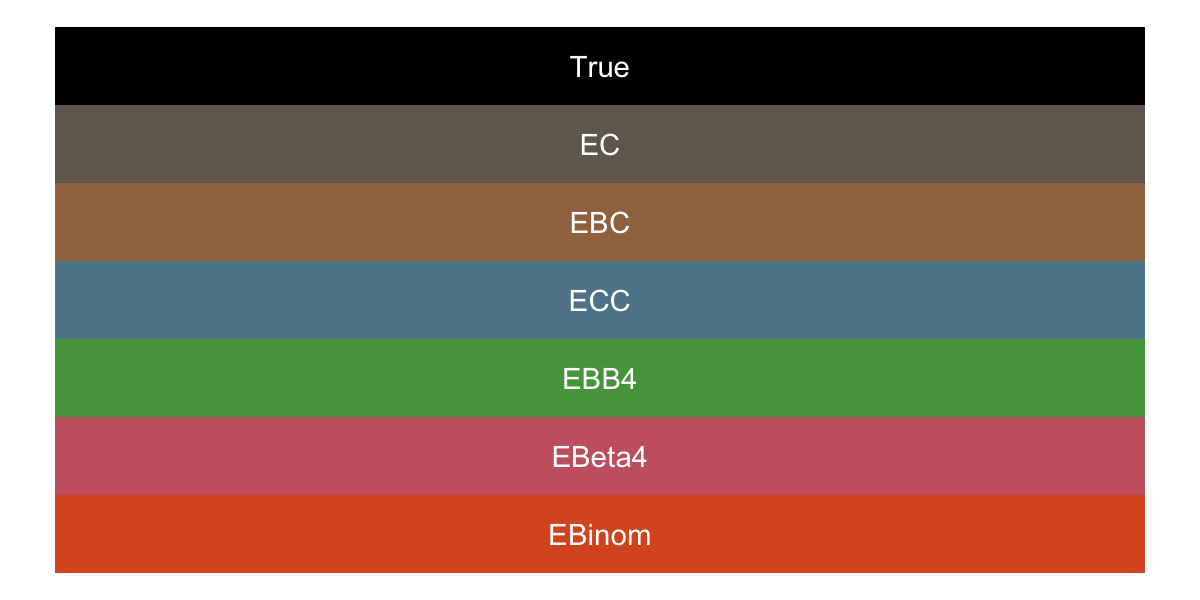
\includegraphics[width=10cm]{ColorPalette/ColorPalette.png}
\caption{Colour code mapping}
\end{figure}%

Notice that some combinations of copula, kendall's tau and dimensions are not plotted. For instance:\\
\vspace{0.5cm}
Recall that the domain of the parameter of Clayton and Gumbel-Hougaard copula is $(0,\infty)$ and $[1,\infty)$ respectively. Consider the kendall's tau for Gumbel-Hougaard and Clayton copulas:
\begin{align*}
    \tau_{C} = \frac{\theta}{\theta + 2}, \: \theta \in (0,\infty) \: \Longrightarrow \: \tau_{C} \in (0,\infty) \\
    \tau_{G} = \frac{\theta - 1}{\theta}, \: \theta \in [1,\infty) \: \Longrightarrow \: \tau_{G} \in [0,\infty) 
\end{align*}
Hence, we will only consider $\tau_{C} \in {0.25, 0.5, 0.75}$ for Clayton copulas and $\tau_{G} \in {0, 0.25, 0.5, 0.75}$.\\
\vspace{0.5cm}
Moreover, the rotated copula for normal and student-t copulas faces Monte Carlo errors for $d \ge 3$ \parencite{HofertBook}, hence we will only consider normal and student-t copulas at $d = 2$.
\newpage
\subsection{Plots: $\textbf{u}$ (evaluation points) vs exceedance probabilities}
\vspace{0.5cm}
We first plot the (upper-tailed) evaluation points against the exceedance probabilities for each empirical copula. The evaluation points are on the x-axis and the exceedance probabilities are on the y-axis.

\begin{center}
\label{t4_2d_s}
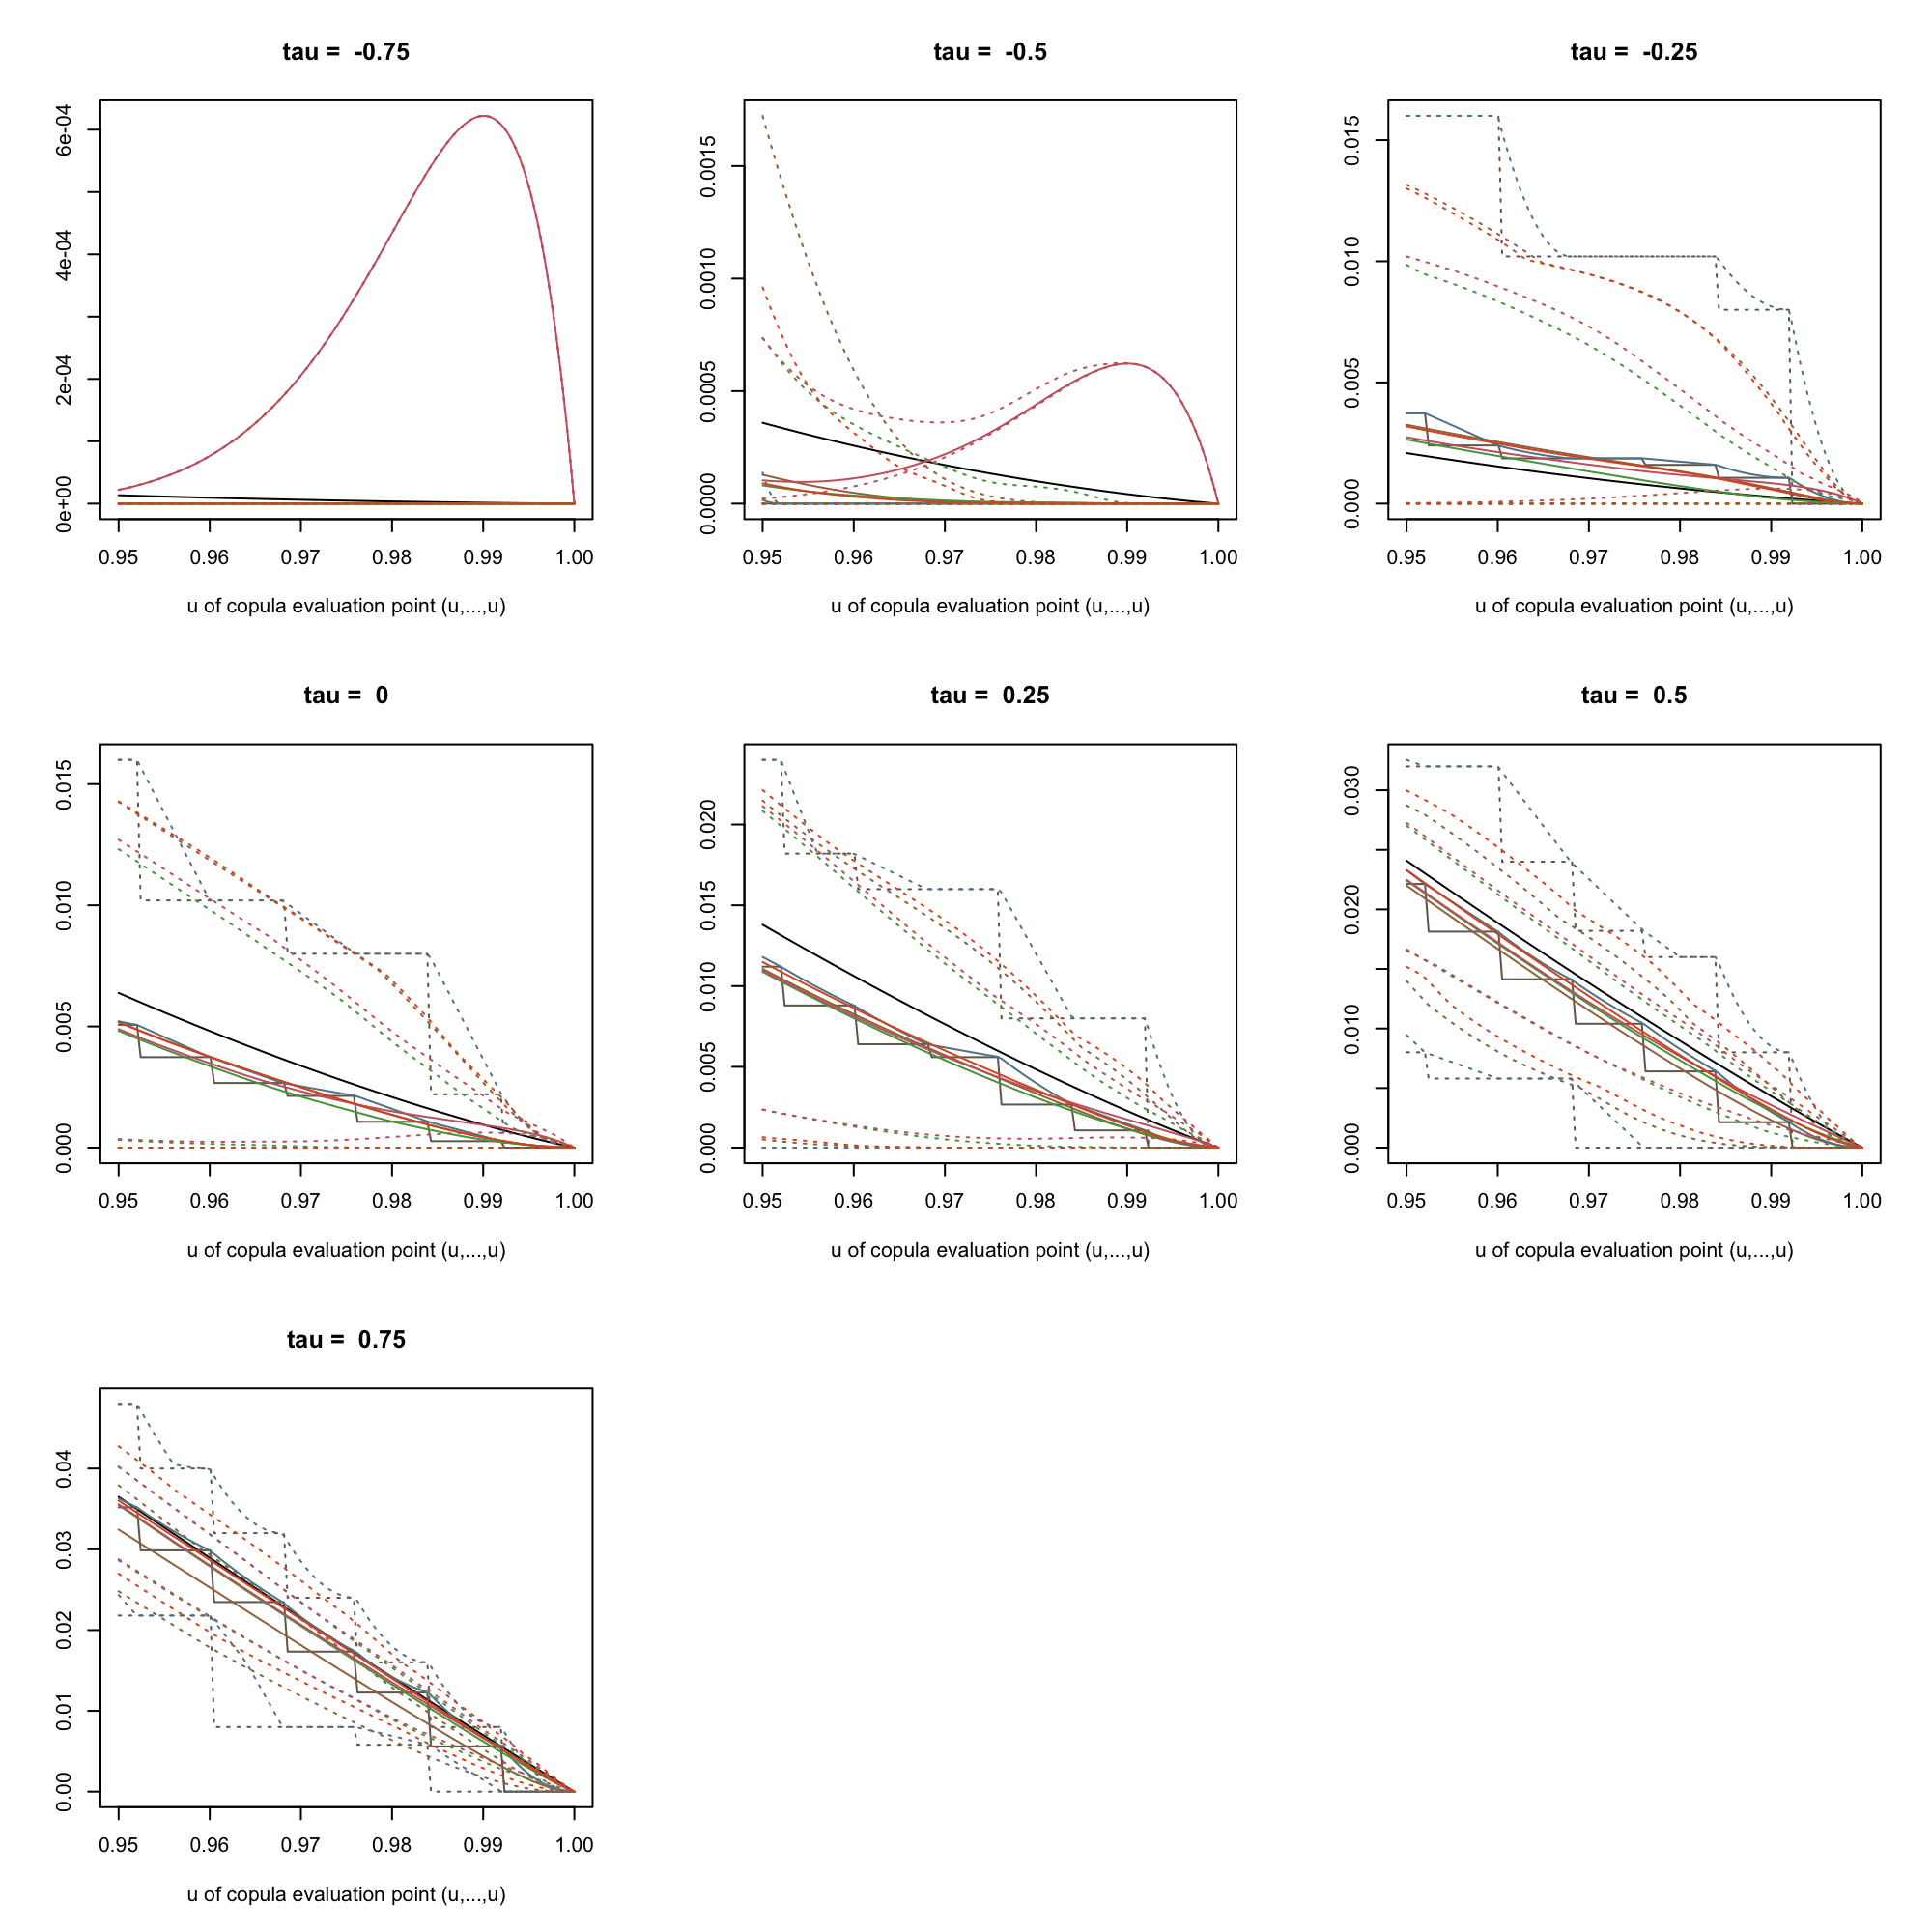
\includegraphics[width=17cm]{ExceedanceProb/t4_2d_s.png}
\captionof{figure}{Student-t copula with d = 2}
\end{center}%

\begin{center}
\label{N_2d_s}
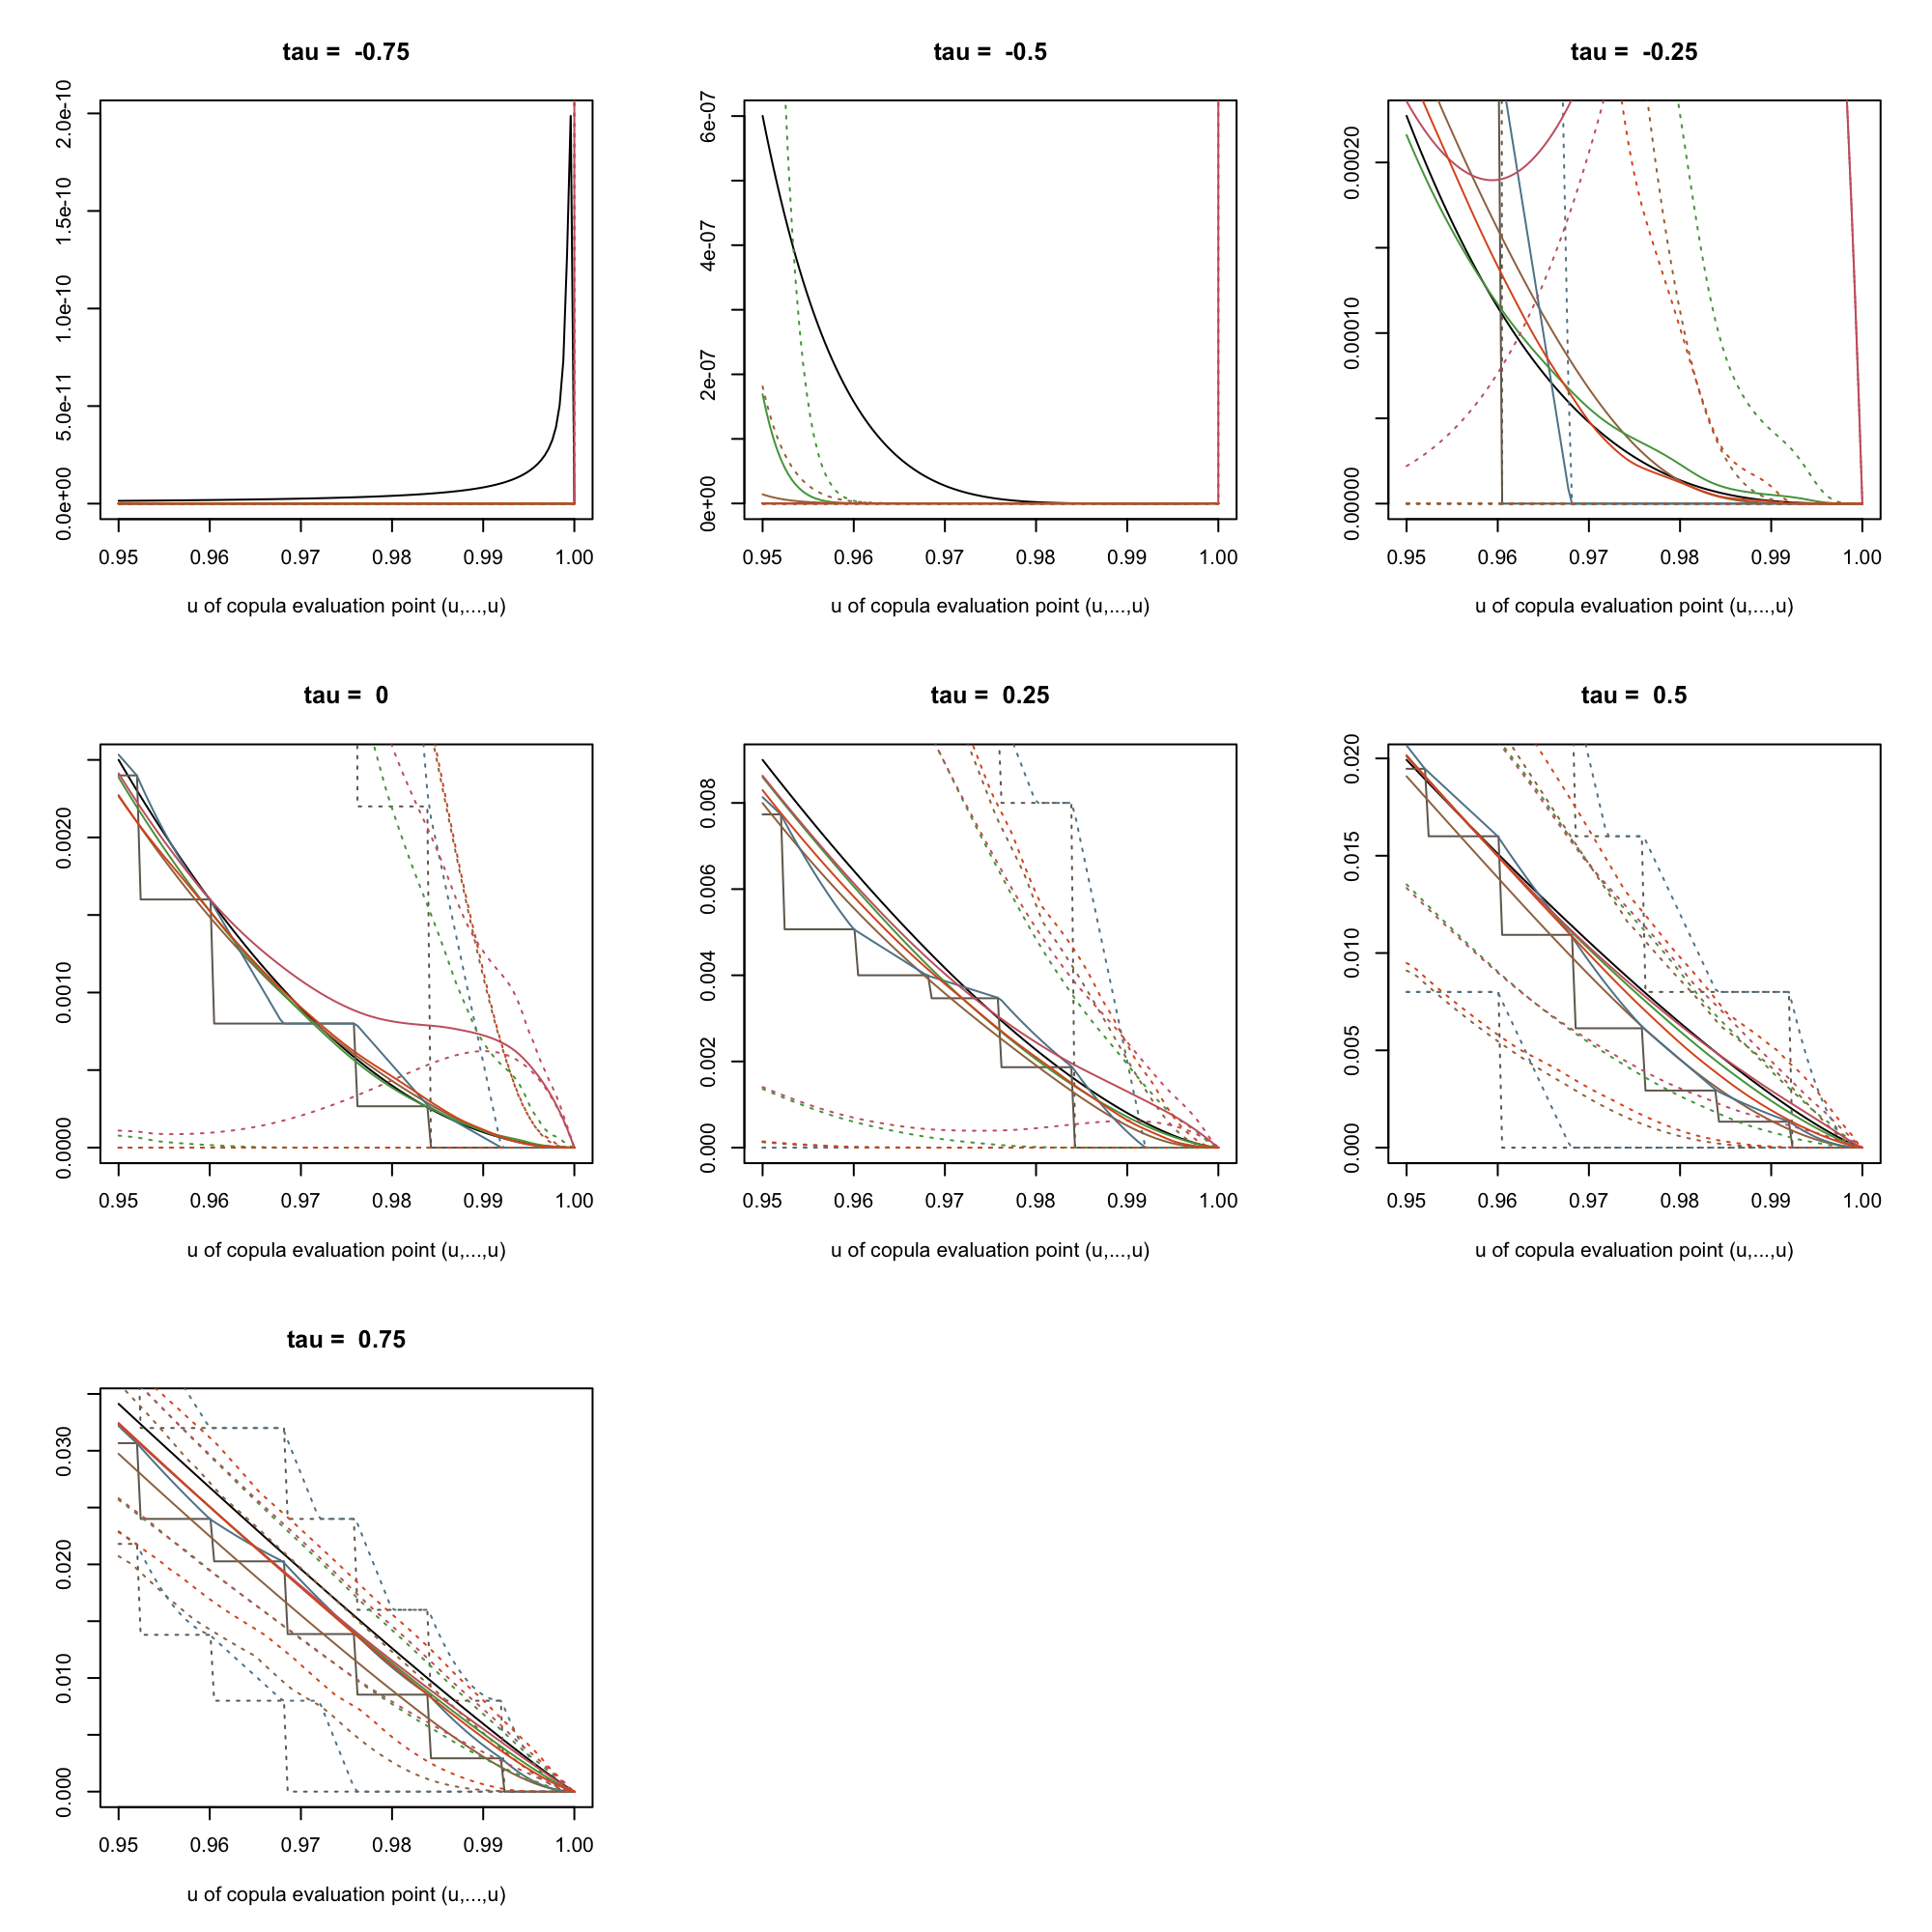
\includegraphics[width=17cm]{ExceedanceProb/N_2d_s.png}
\captionof{figure}{Gaussian copula with d = 2}
\end{center}%

\begin{center}
\label{G_2d_s}
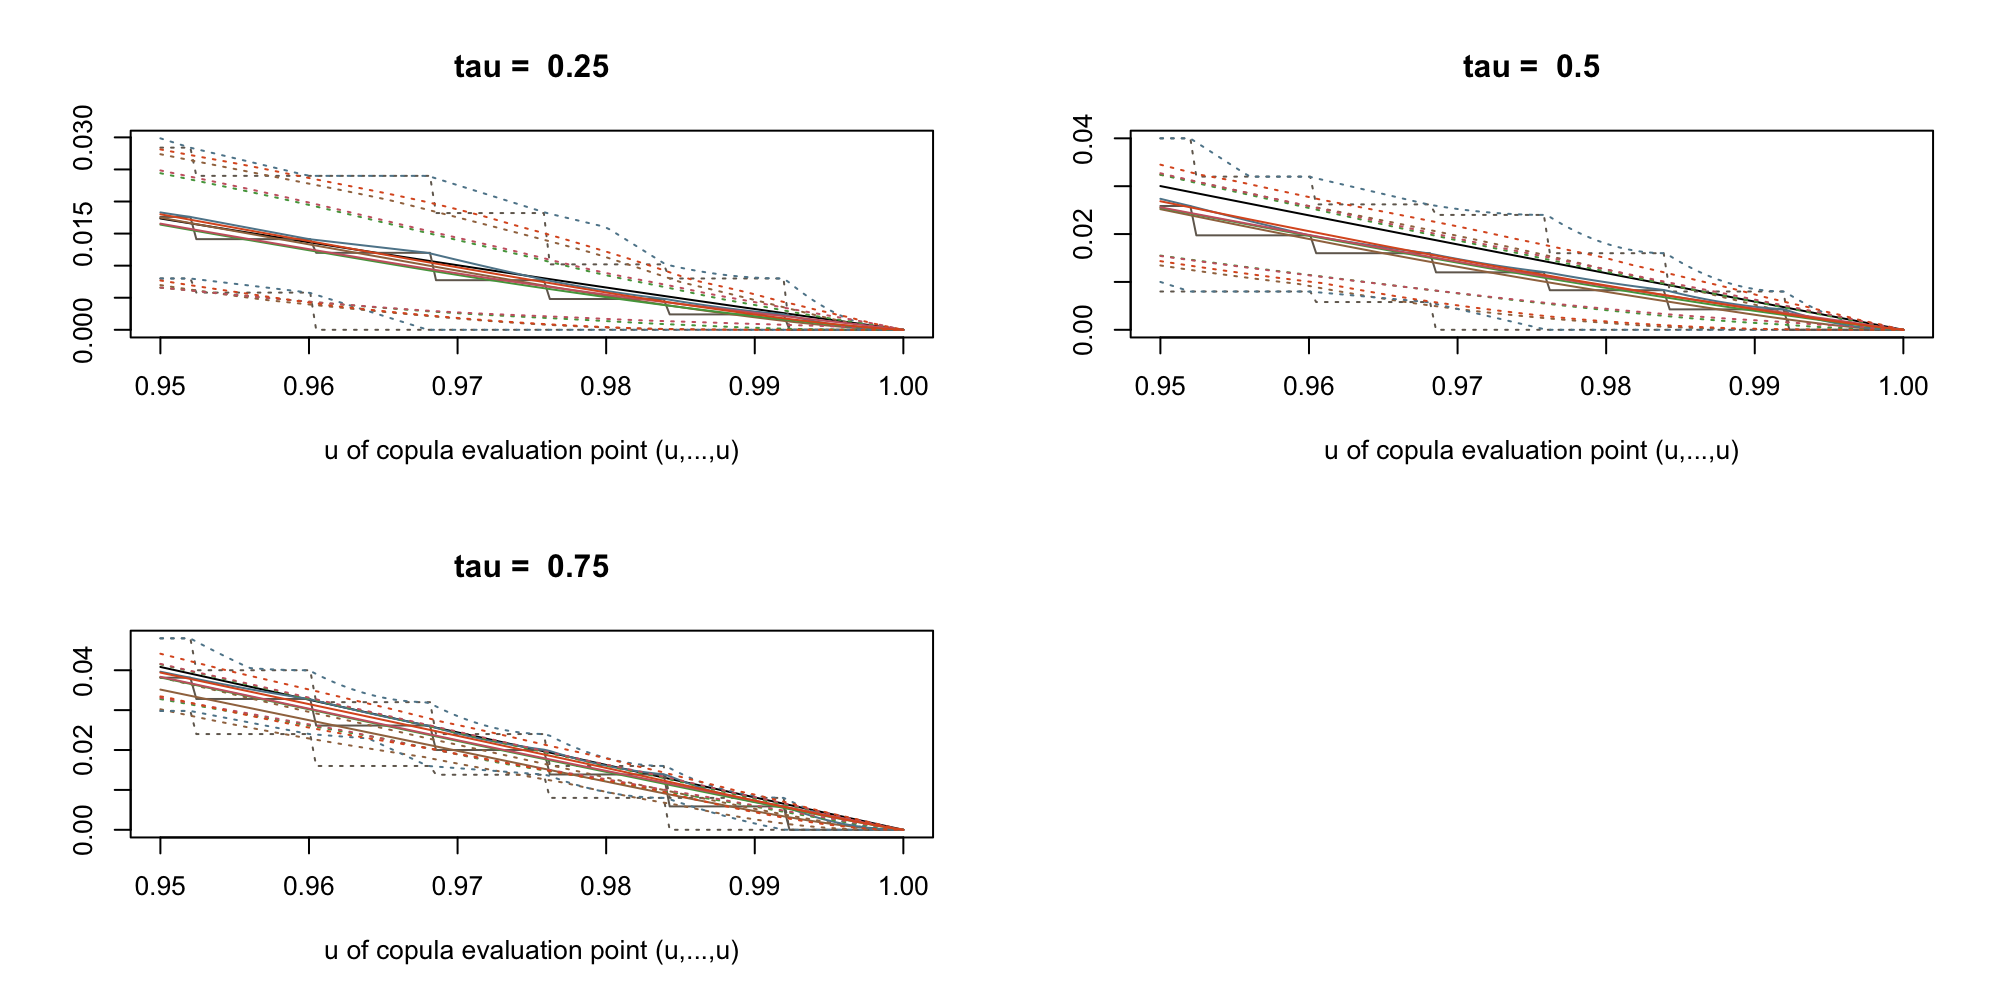
\includegraphics[width=17cm]{ExceedanceProb/G_2d_s.png}
\captionof{figure}{Gumbel-Hougaard copula with d = 2}
\end{center}%

\begin{center}
\label{G_3d_s}
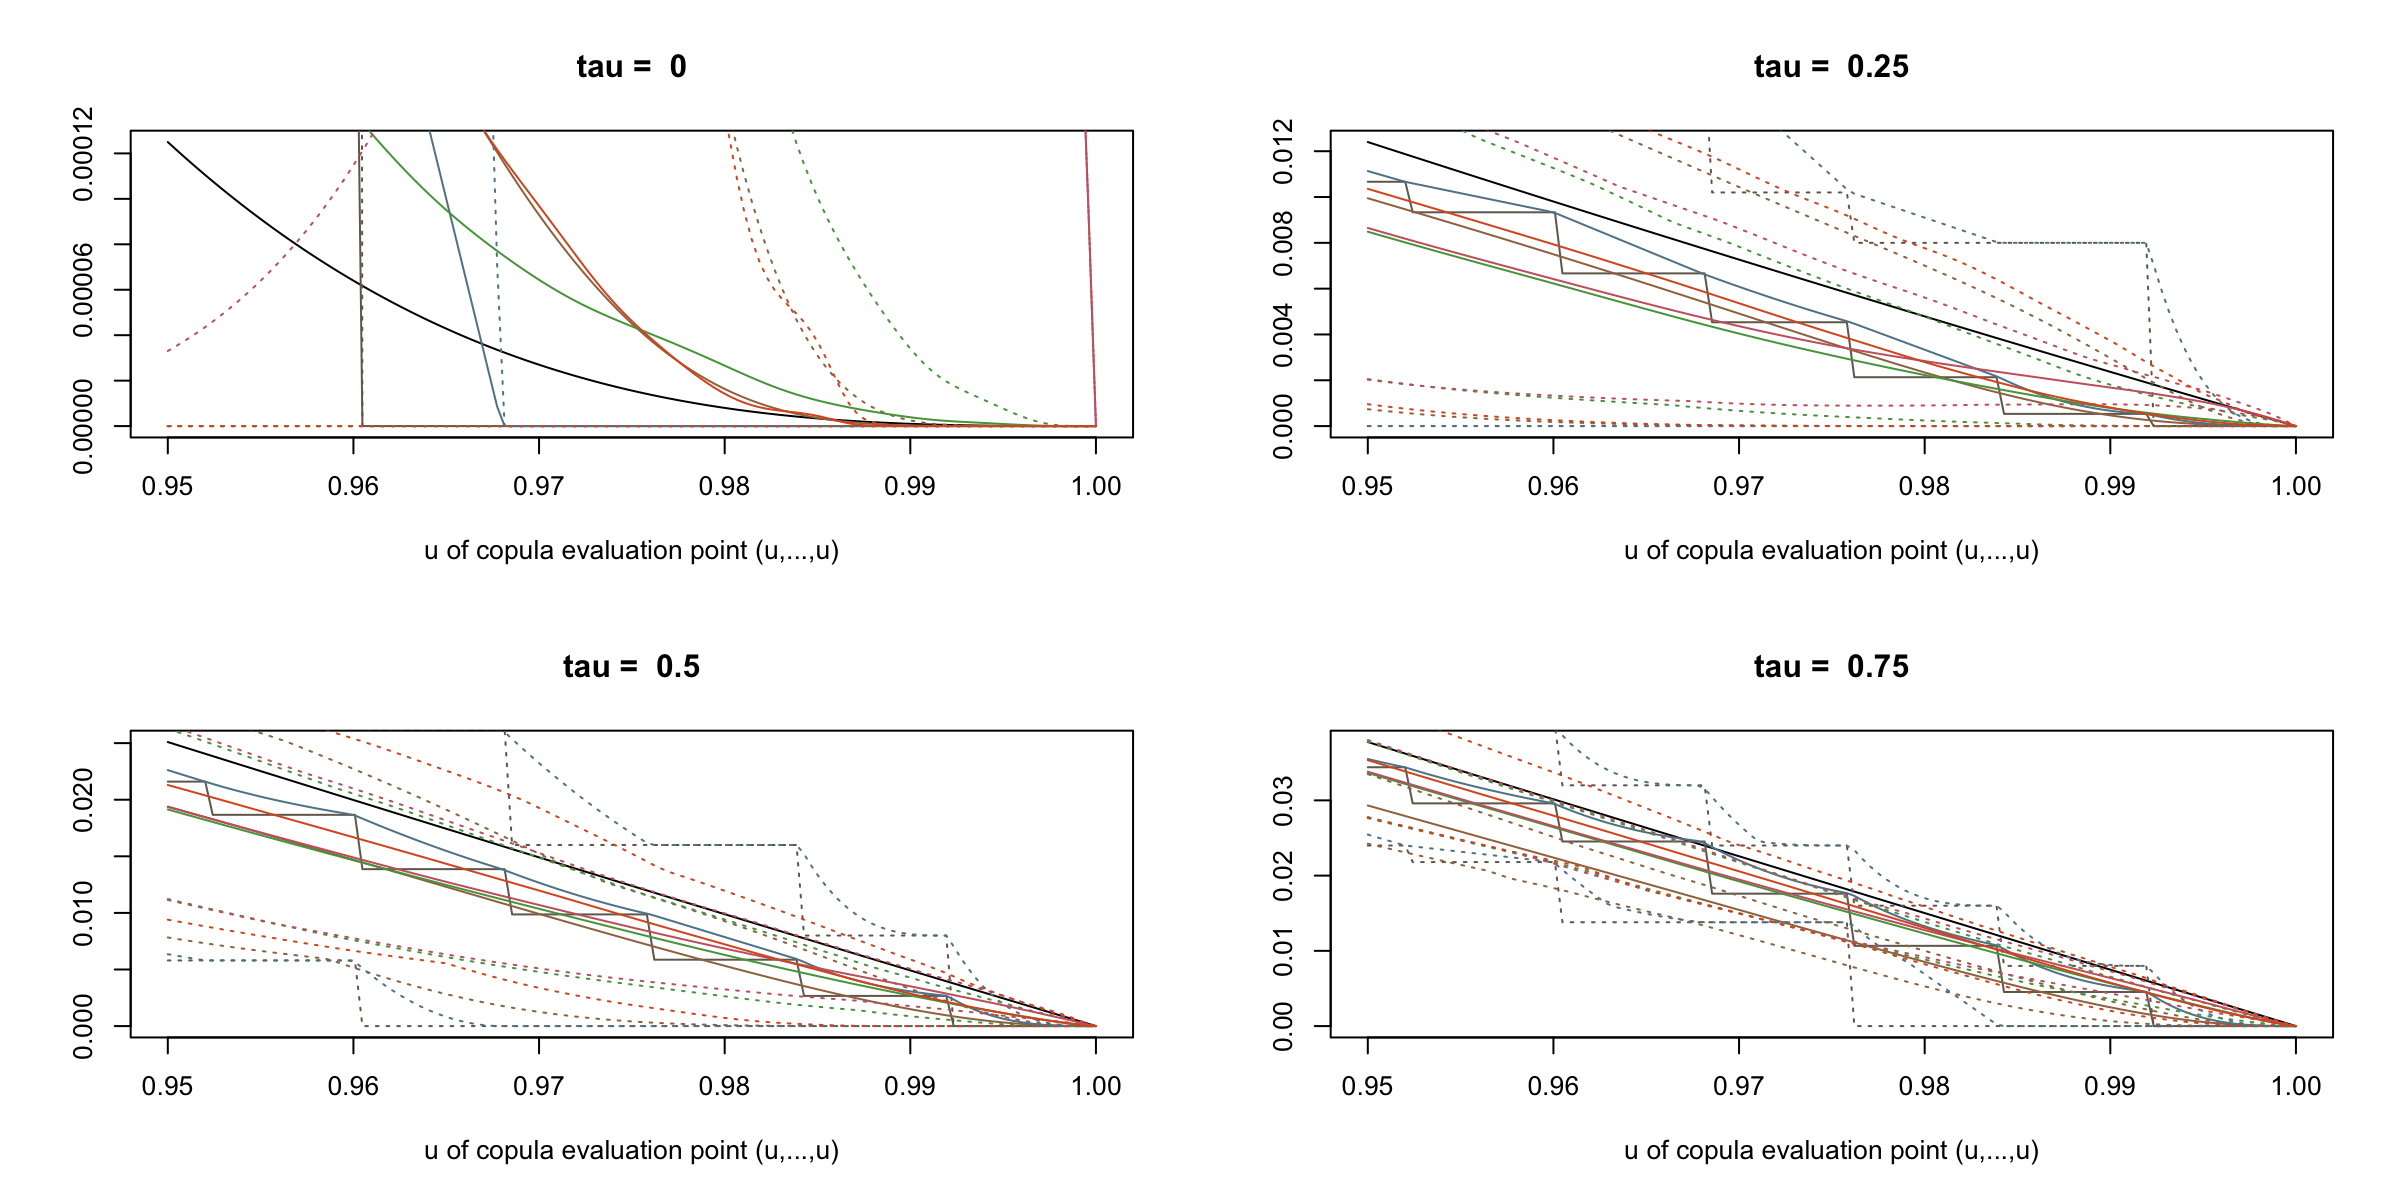
\includegraphics[width=17cm]{ExceedanceProb/G_3d_s.png}
\captionof{figure}{Gumbel-Hougaard copula with d = 3}
\end{center}%

\begin{center}
\label{G_4d_s}
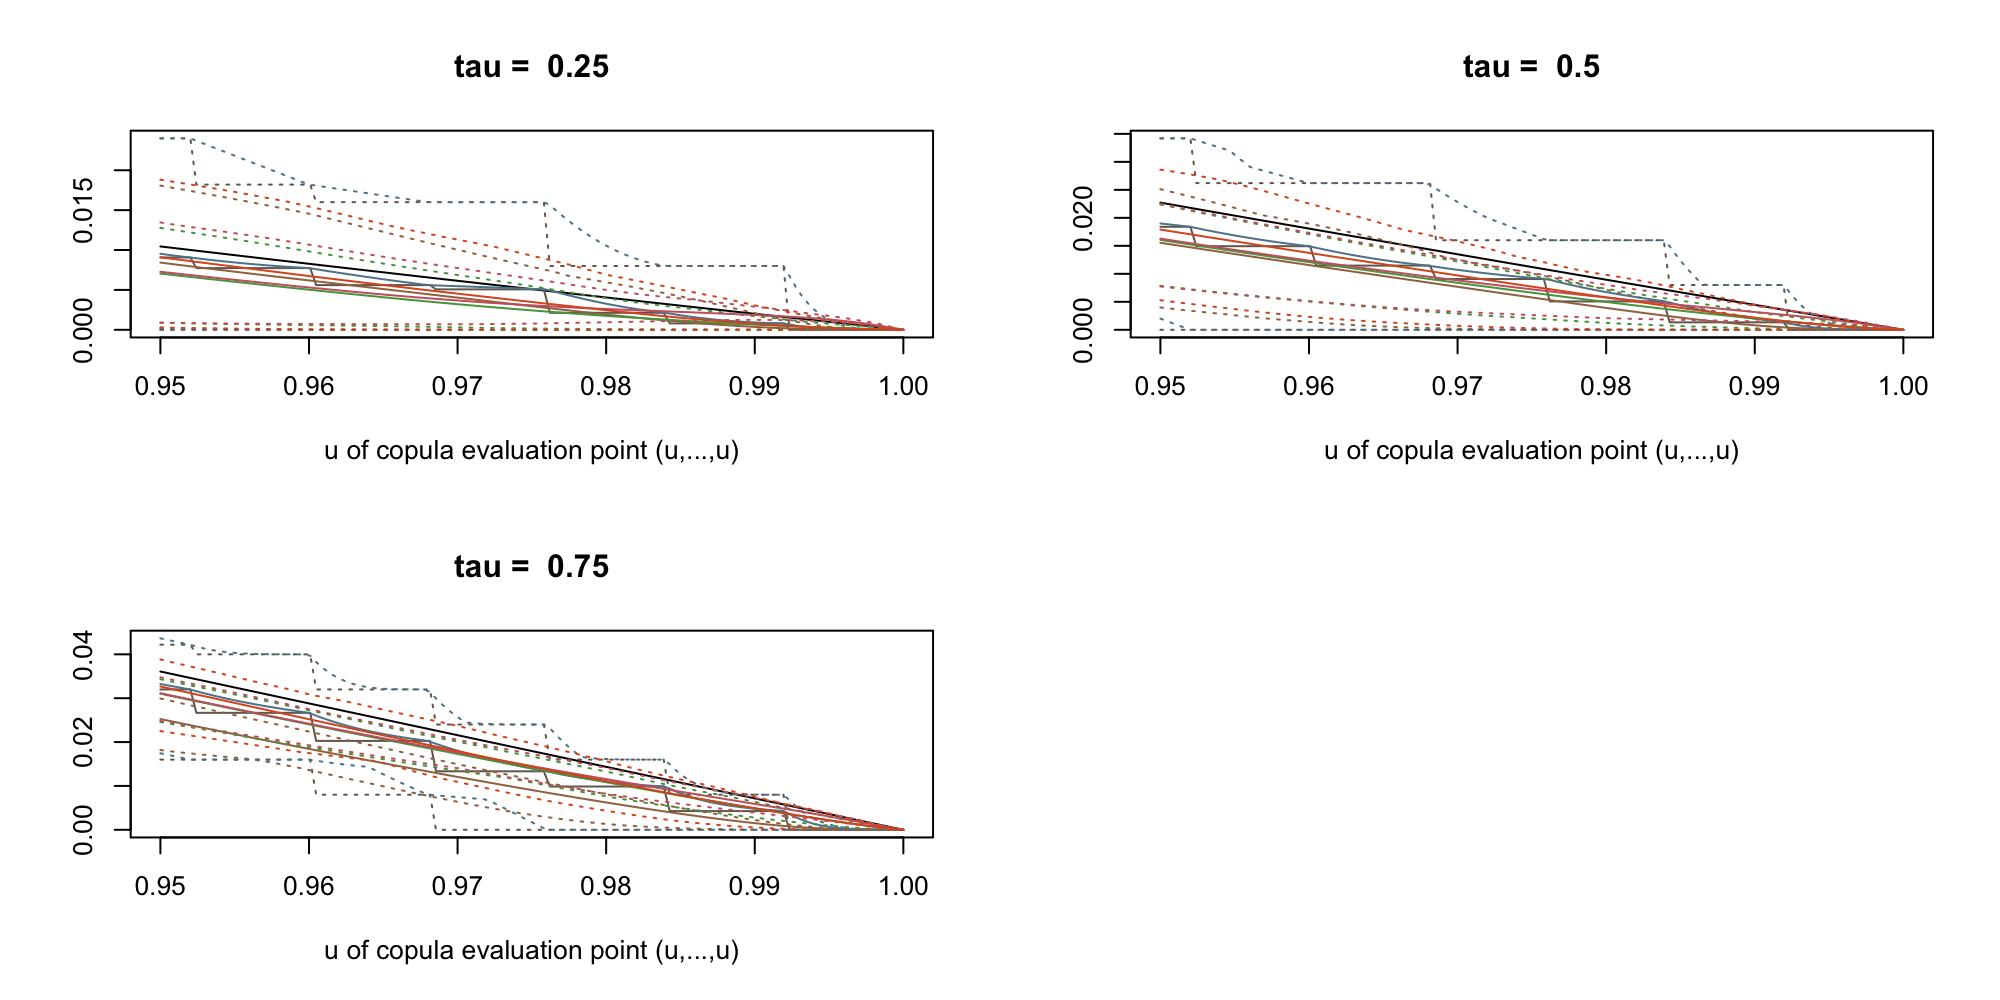
\includegraphics[width=17cm]{ExceedanceProb/G_4d_s.png}
\captionof{figure}{Gumbel-Hougaard copula with d = 4}
\end{center}%

\begin{center}
\label{G_5d_s}
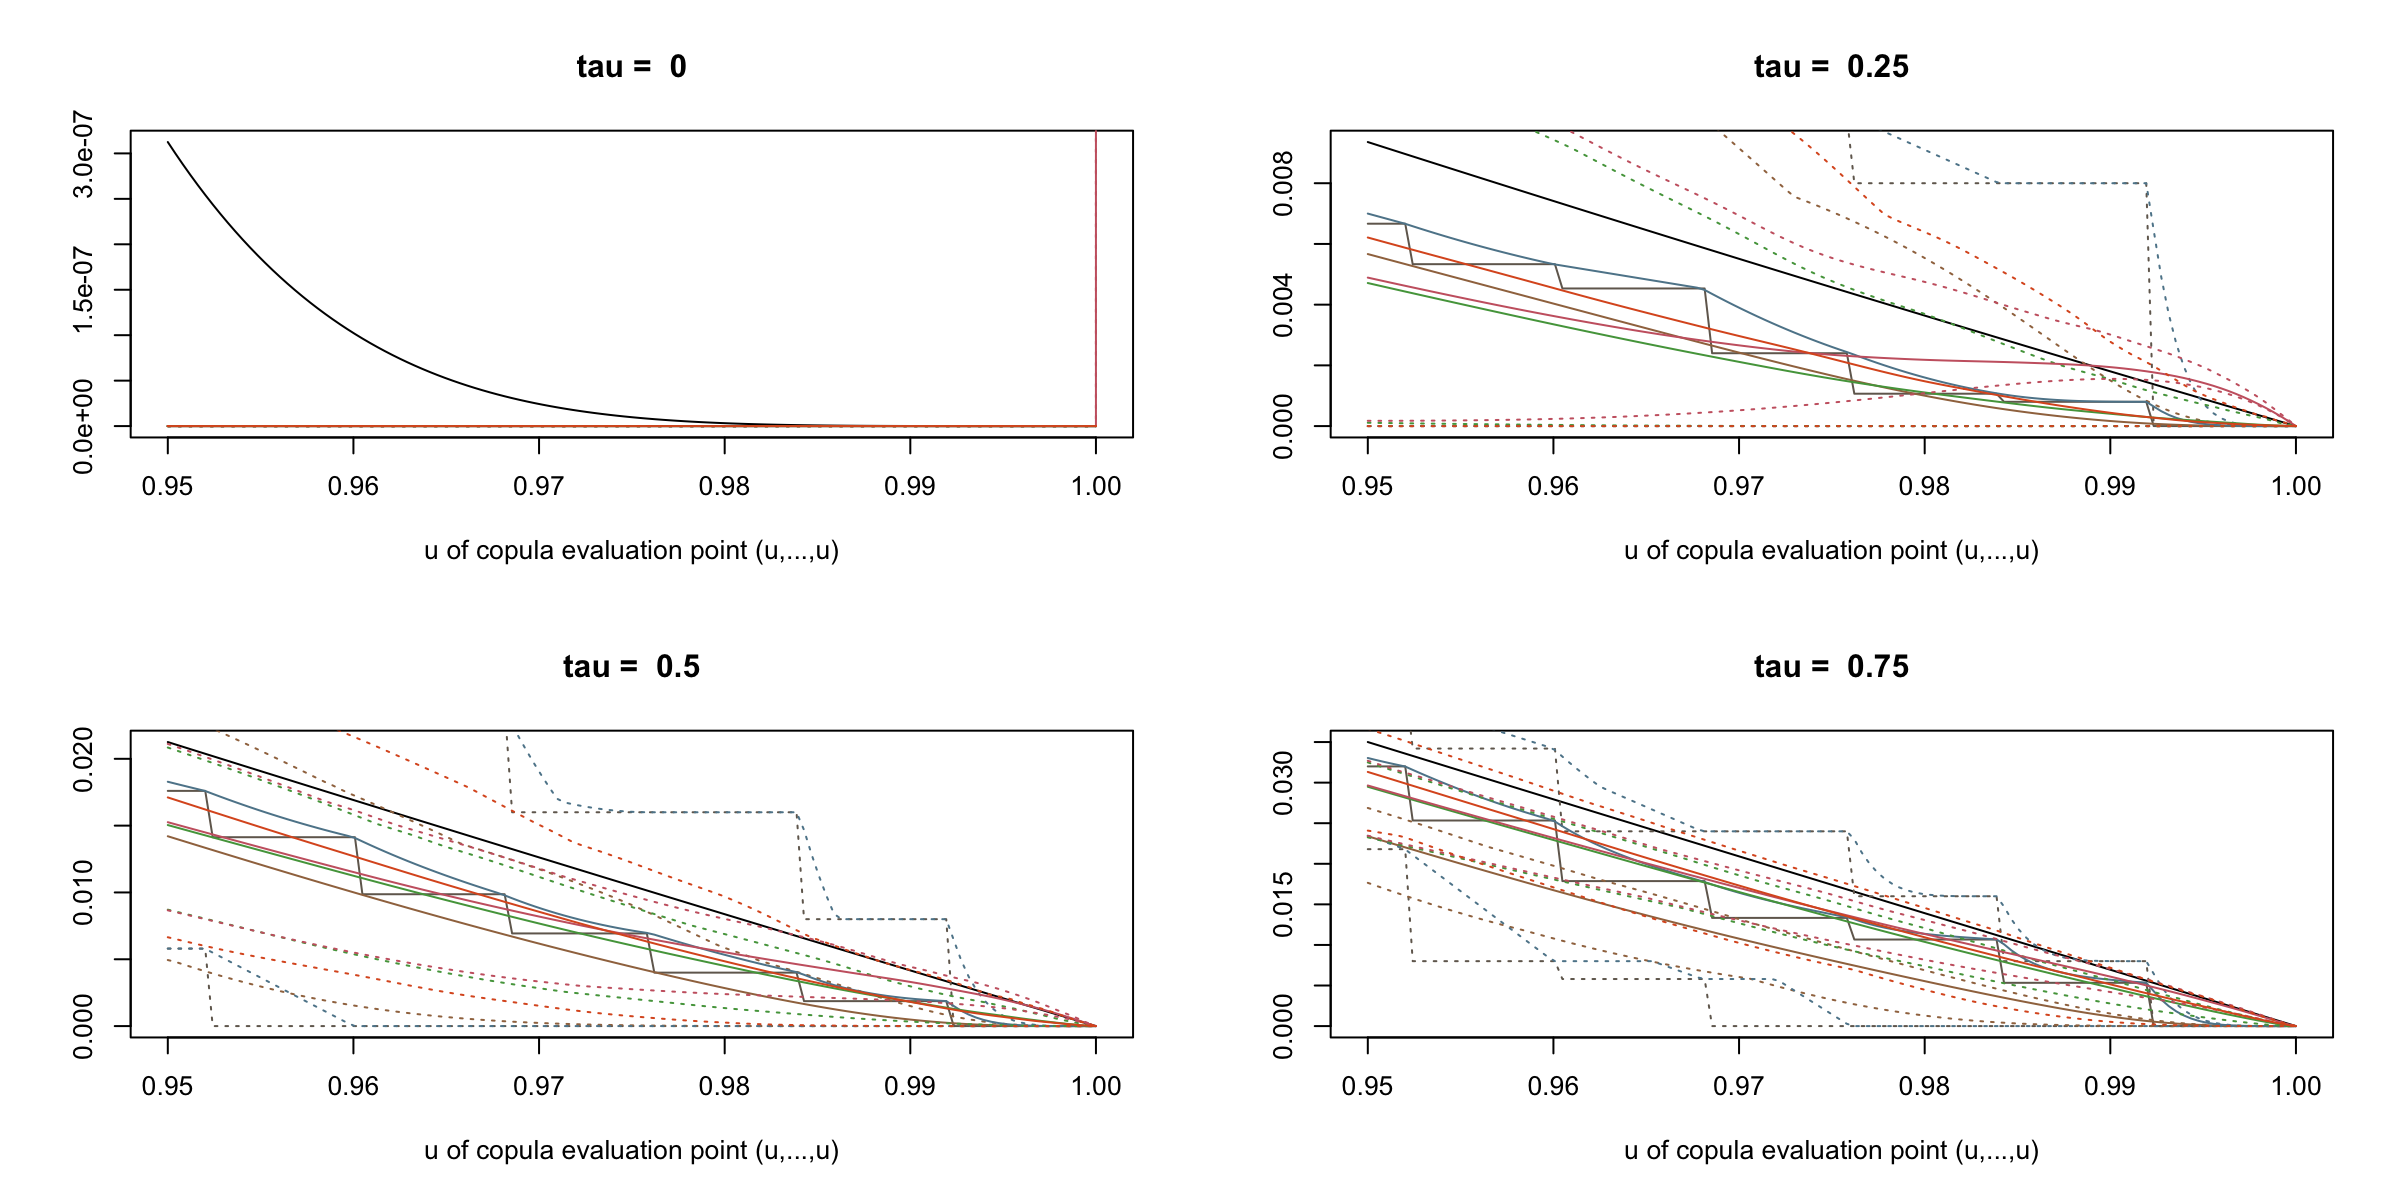
\includegraphics[width=17cm]{ExceedanceProb/G_5d_s.png}
\captionof{figure}{Gumbel-Hougaard copula with d = 5}
\end{center}%

\newpage
\subsection{CvM: Exceedance probabilities}
To better understand the proximity of the exceedance probabilities from the class of empirical copula, with respect to the true copula, we then compute the Cramer-von-Mises statistics for all combinations of empirical copulas, Kendall's Tau and dimensions.

\begin{center}
\label{t4_2d_s_CvM}
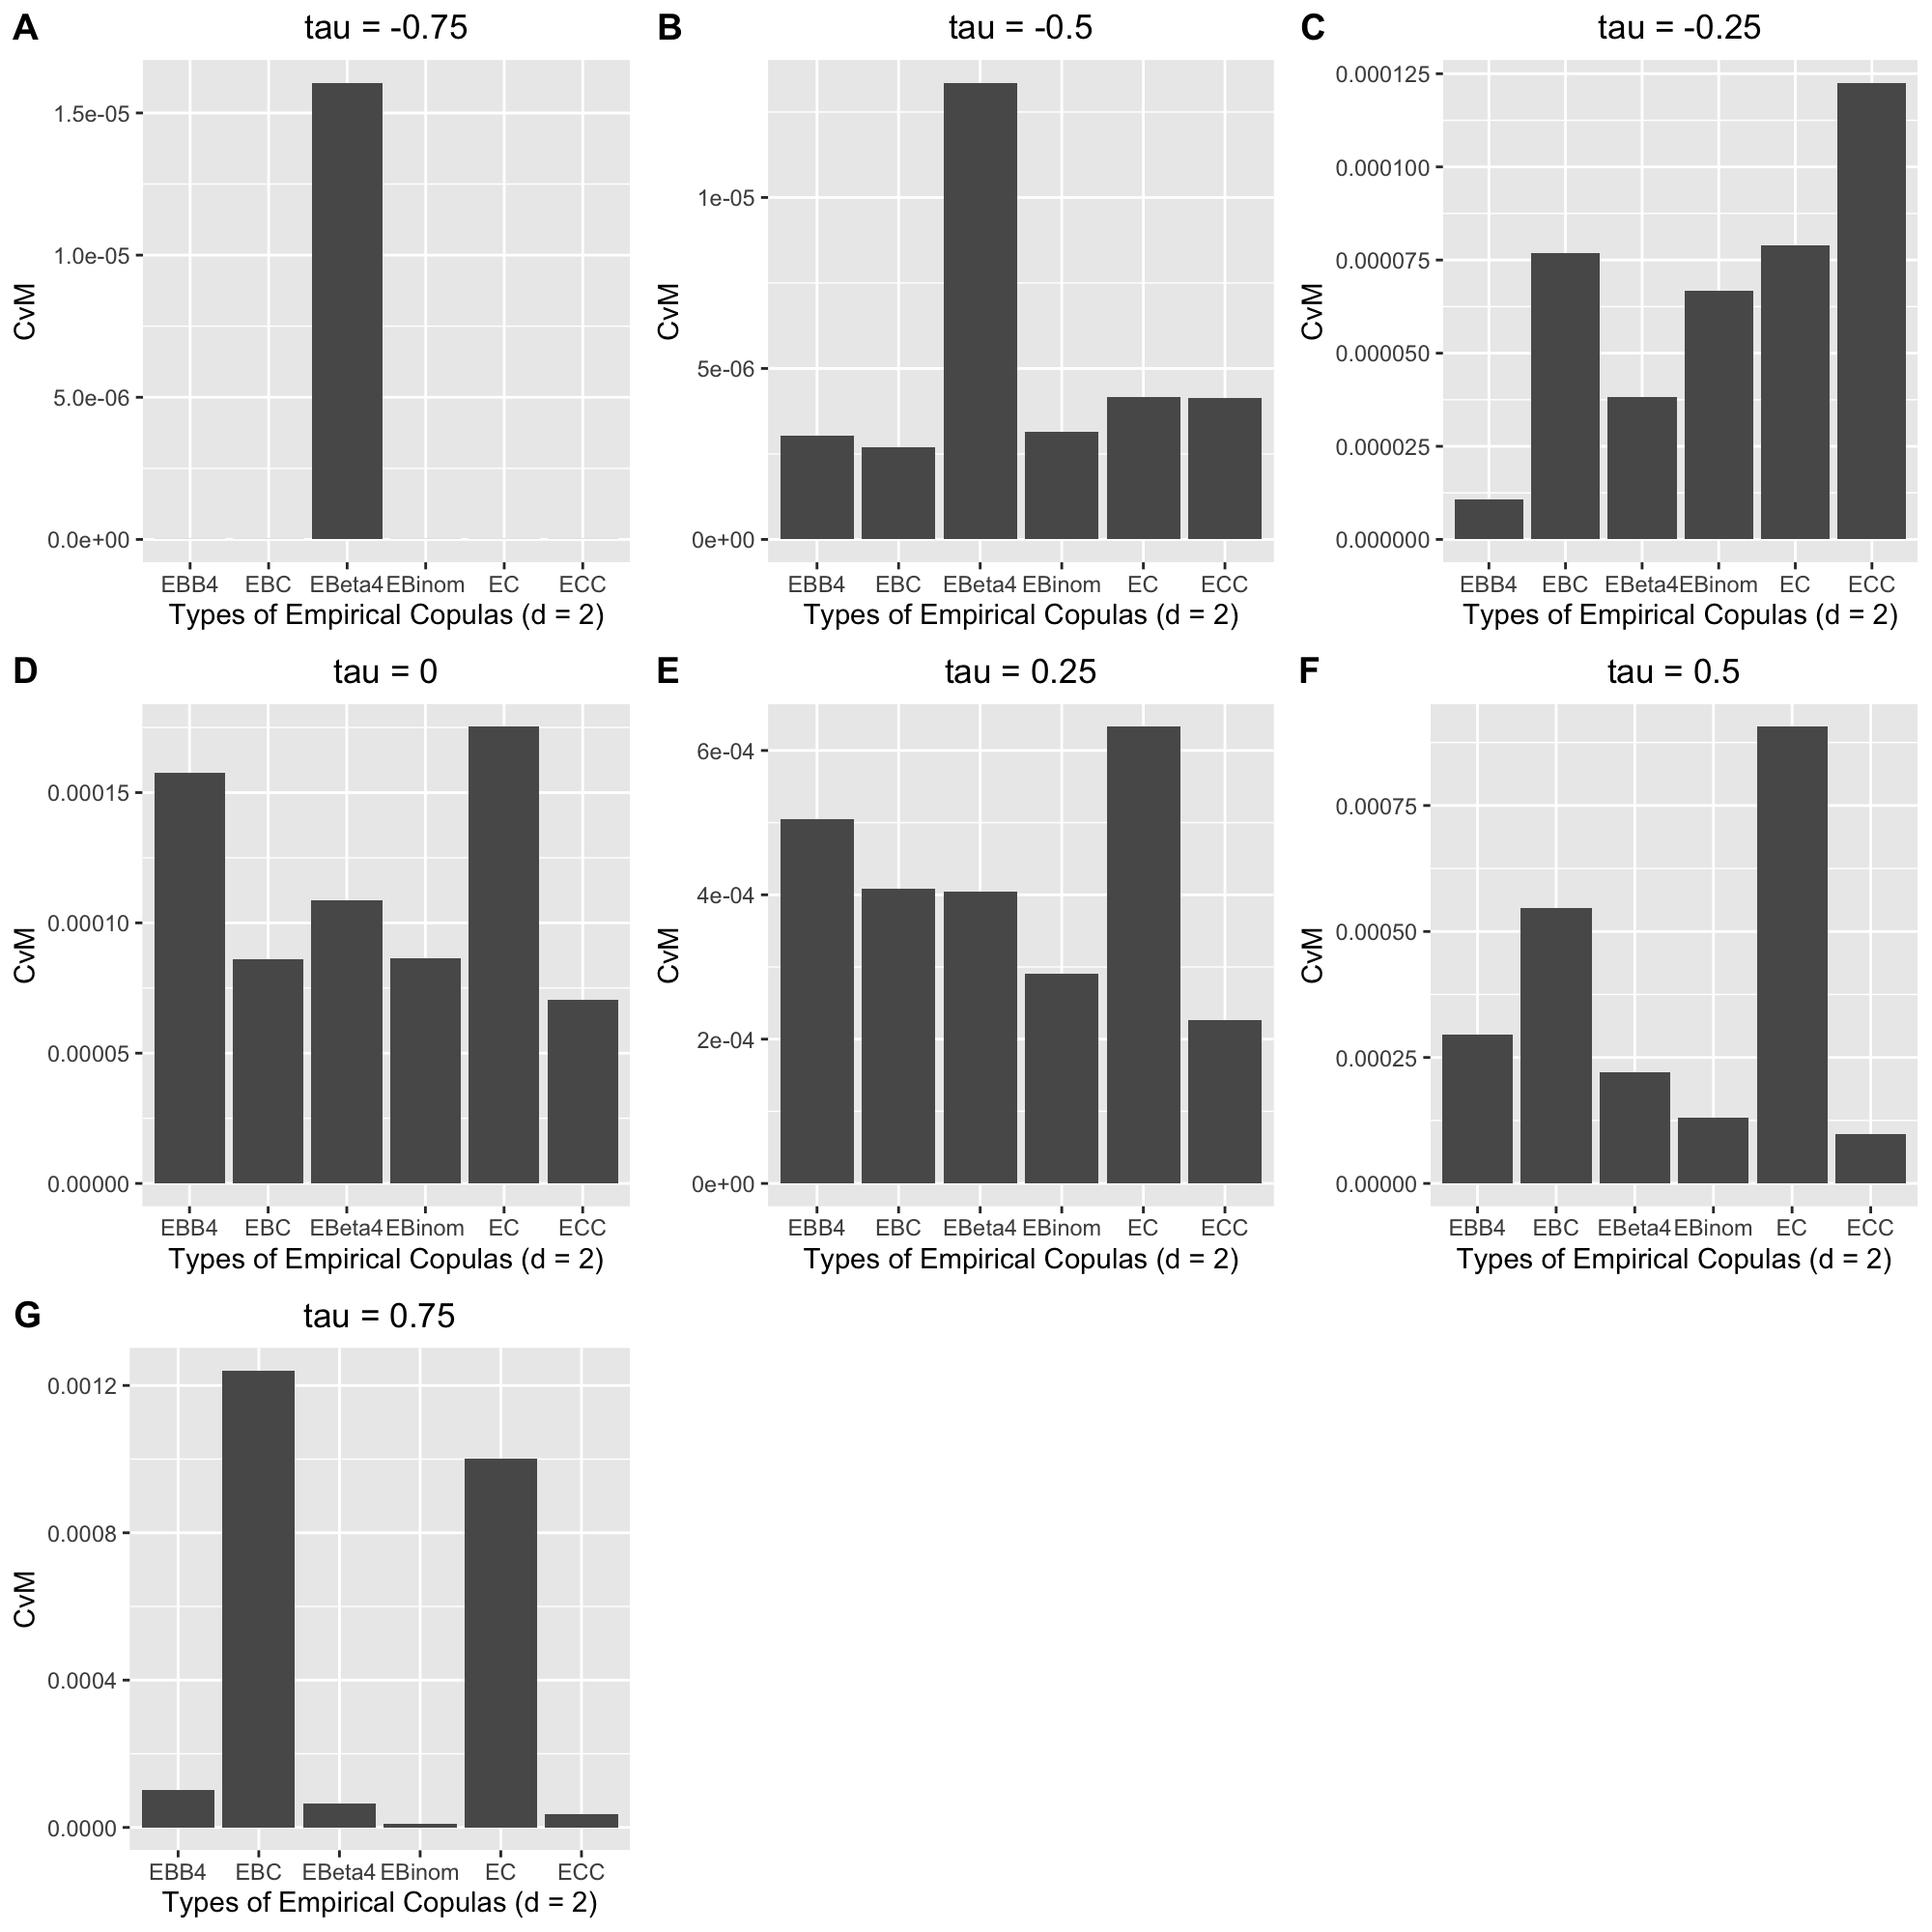
\includegraphics[width=17cm]{ExceedanceCvM/t4_2d_s_CvM.png}
\captionof{figure}{Student-t copula with d = 2}
\end{center}%

\begin{center}
\label{N_2d_s_CvM}
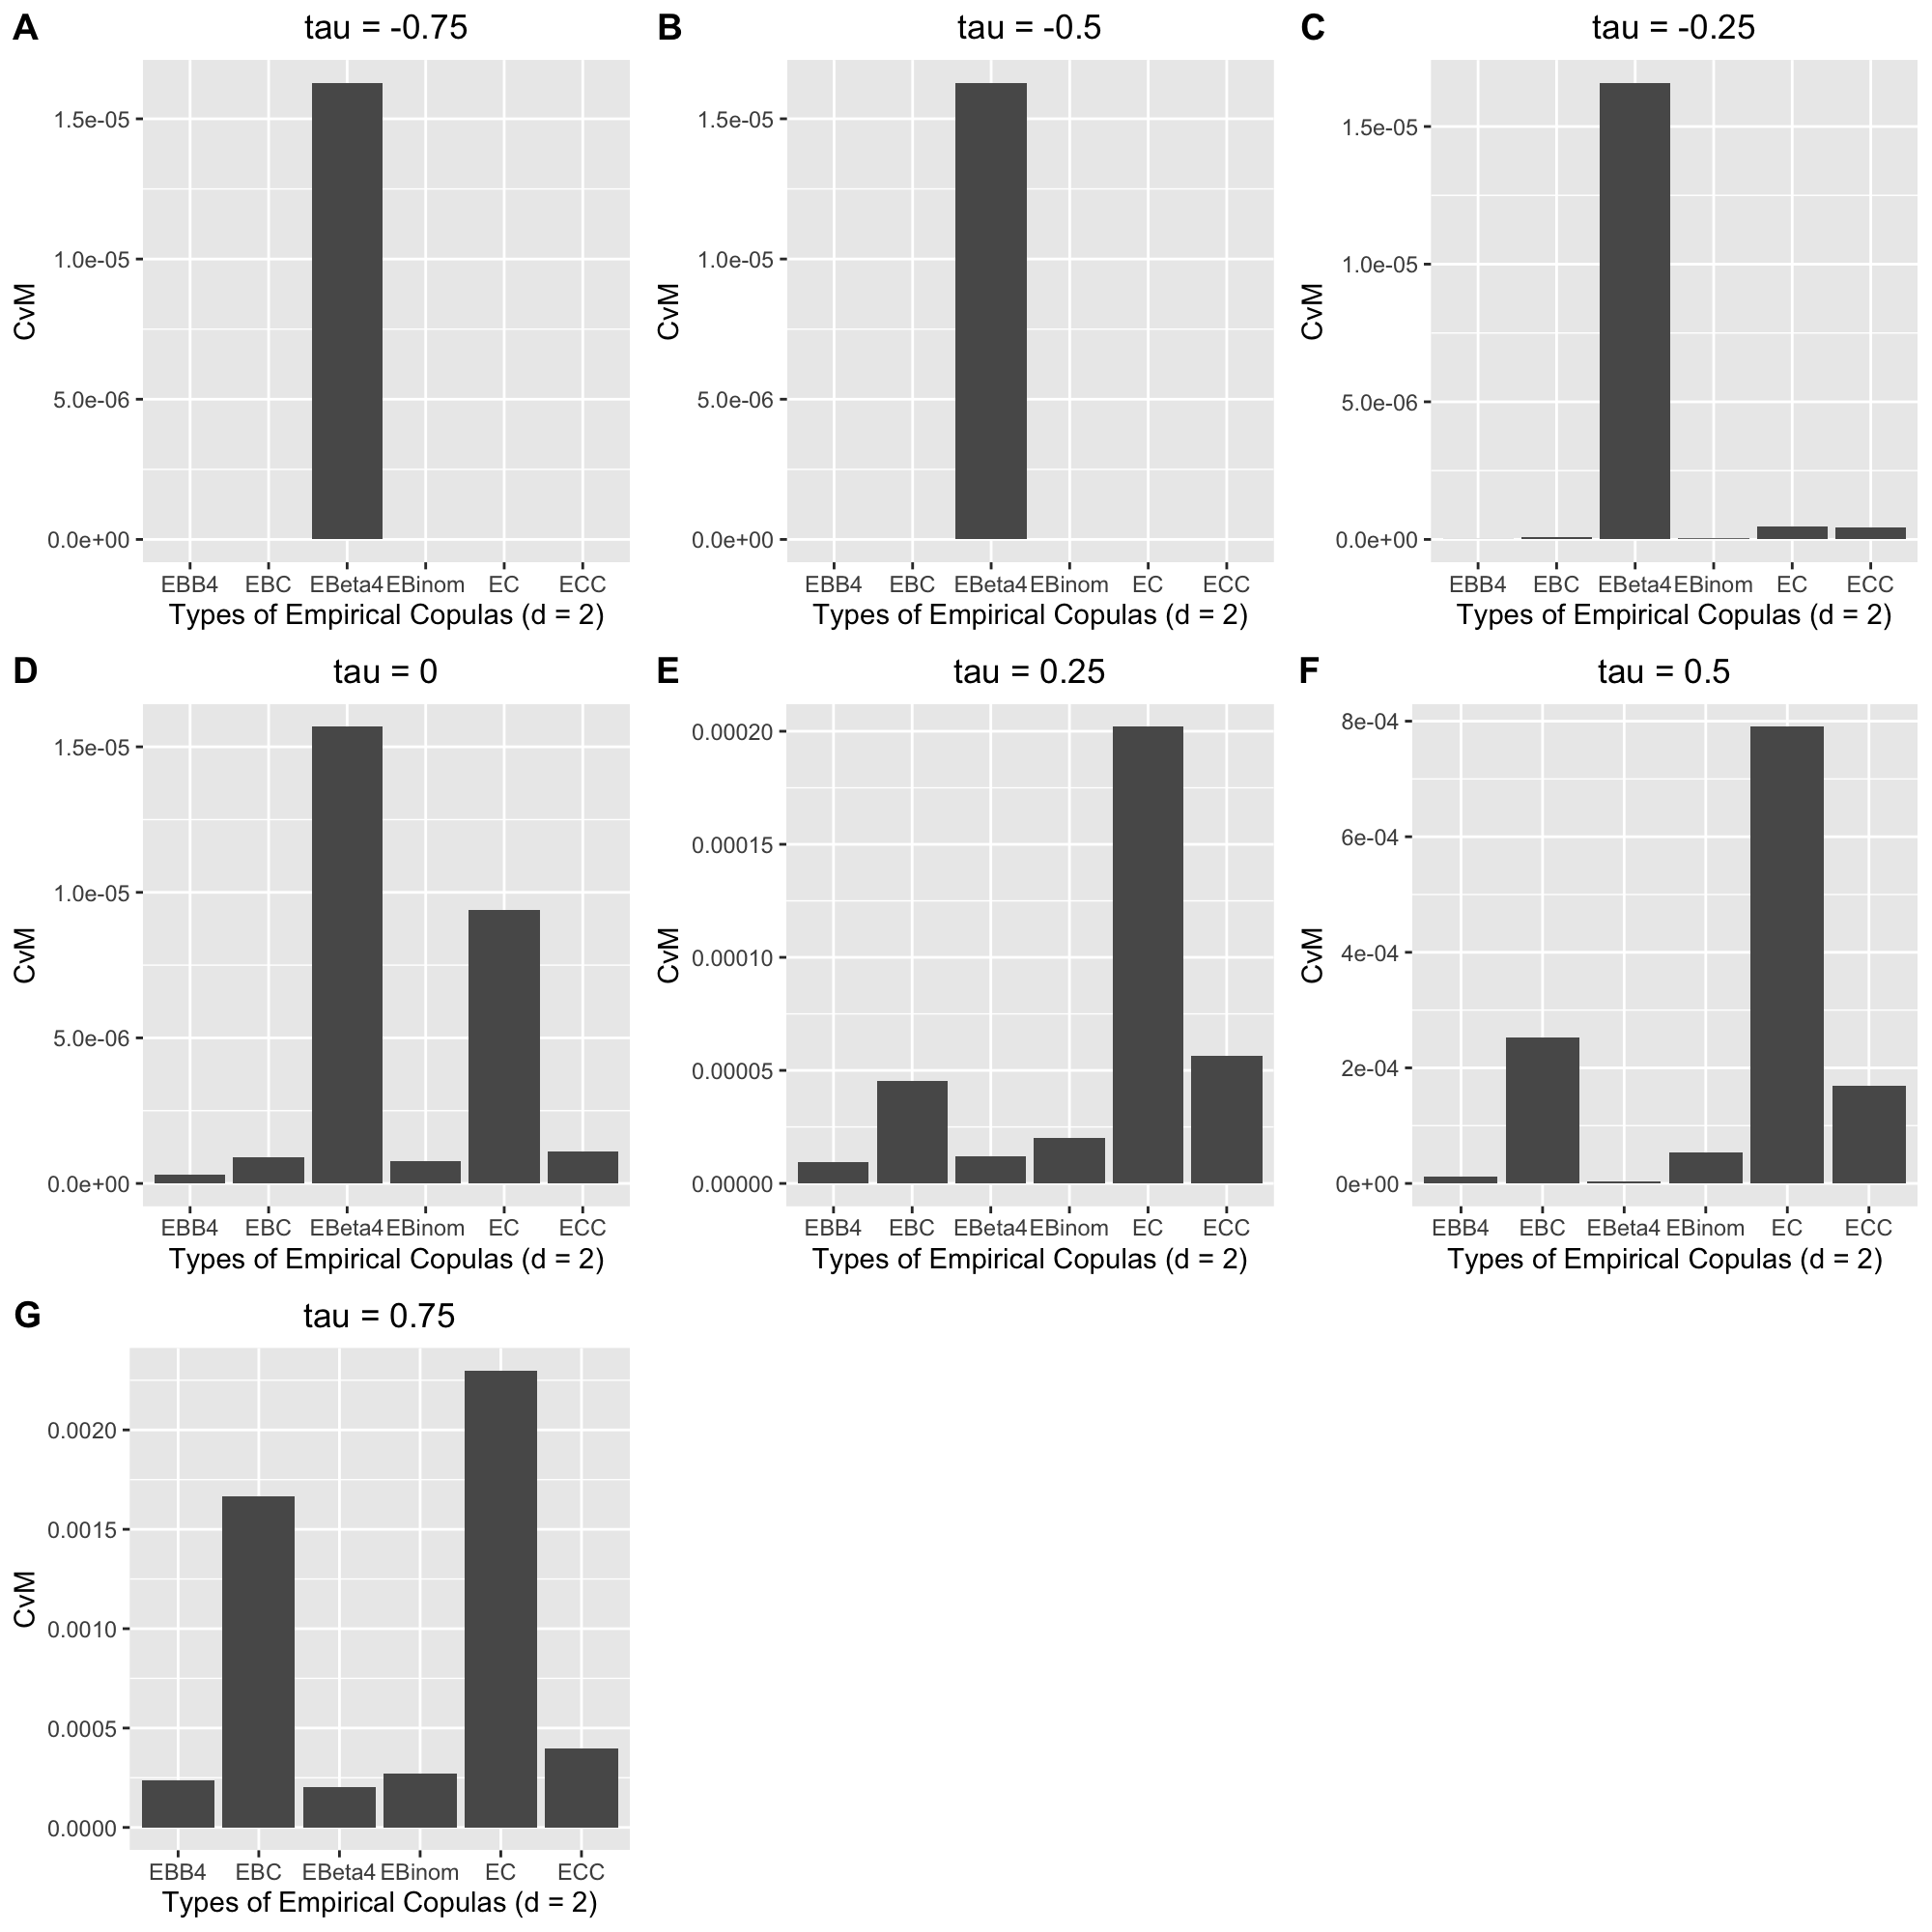
\includegraphics[width=17cm]{ExceedanceCvM/N_2d_s_CvM.png}
\captionof{figure}{Gaussian copula with d = 2}
\end{center}%

\begin{center}
\label{G_2d_s_CvM}
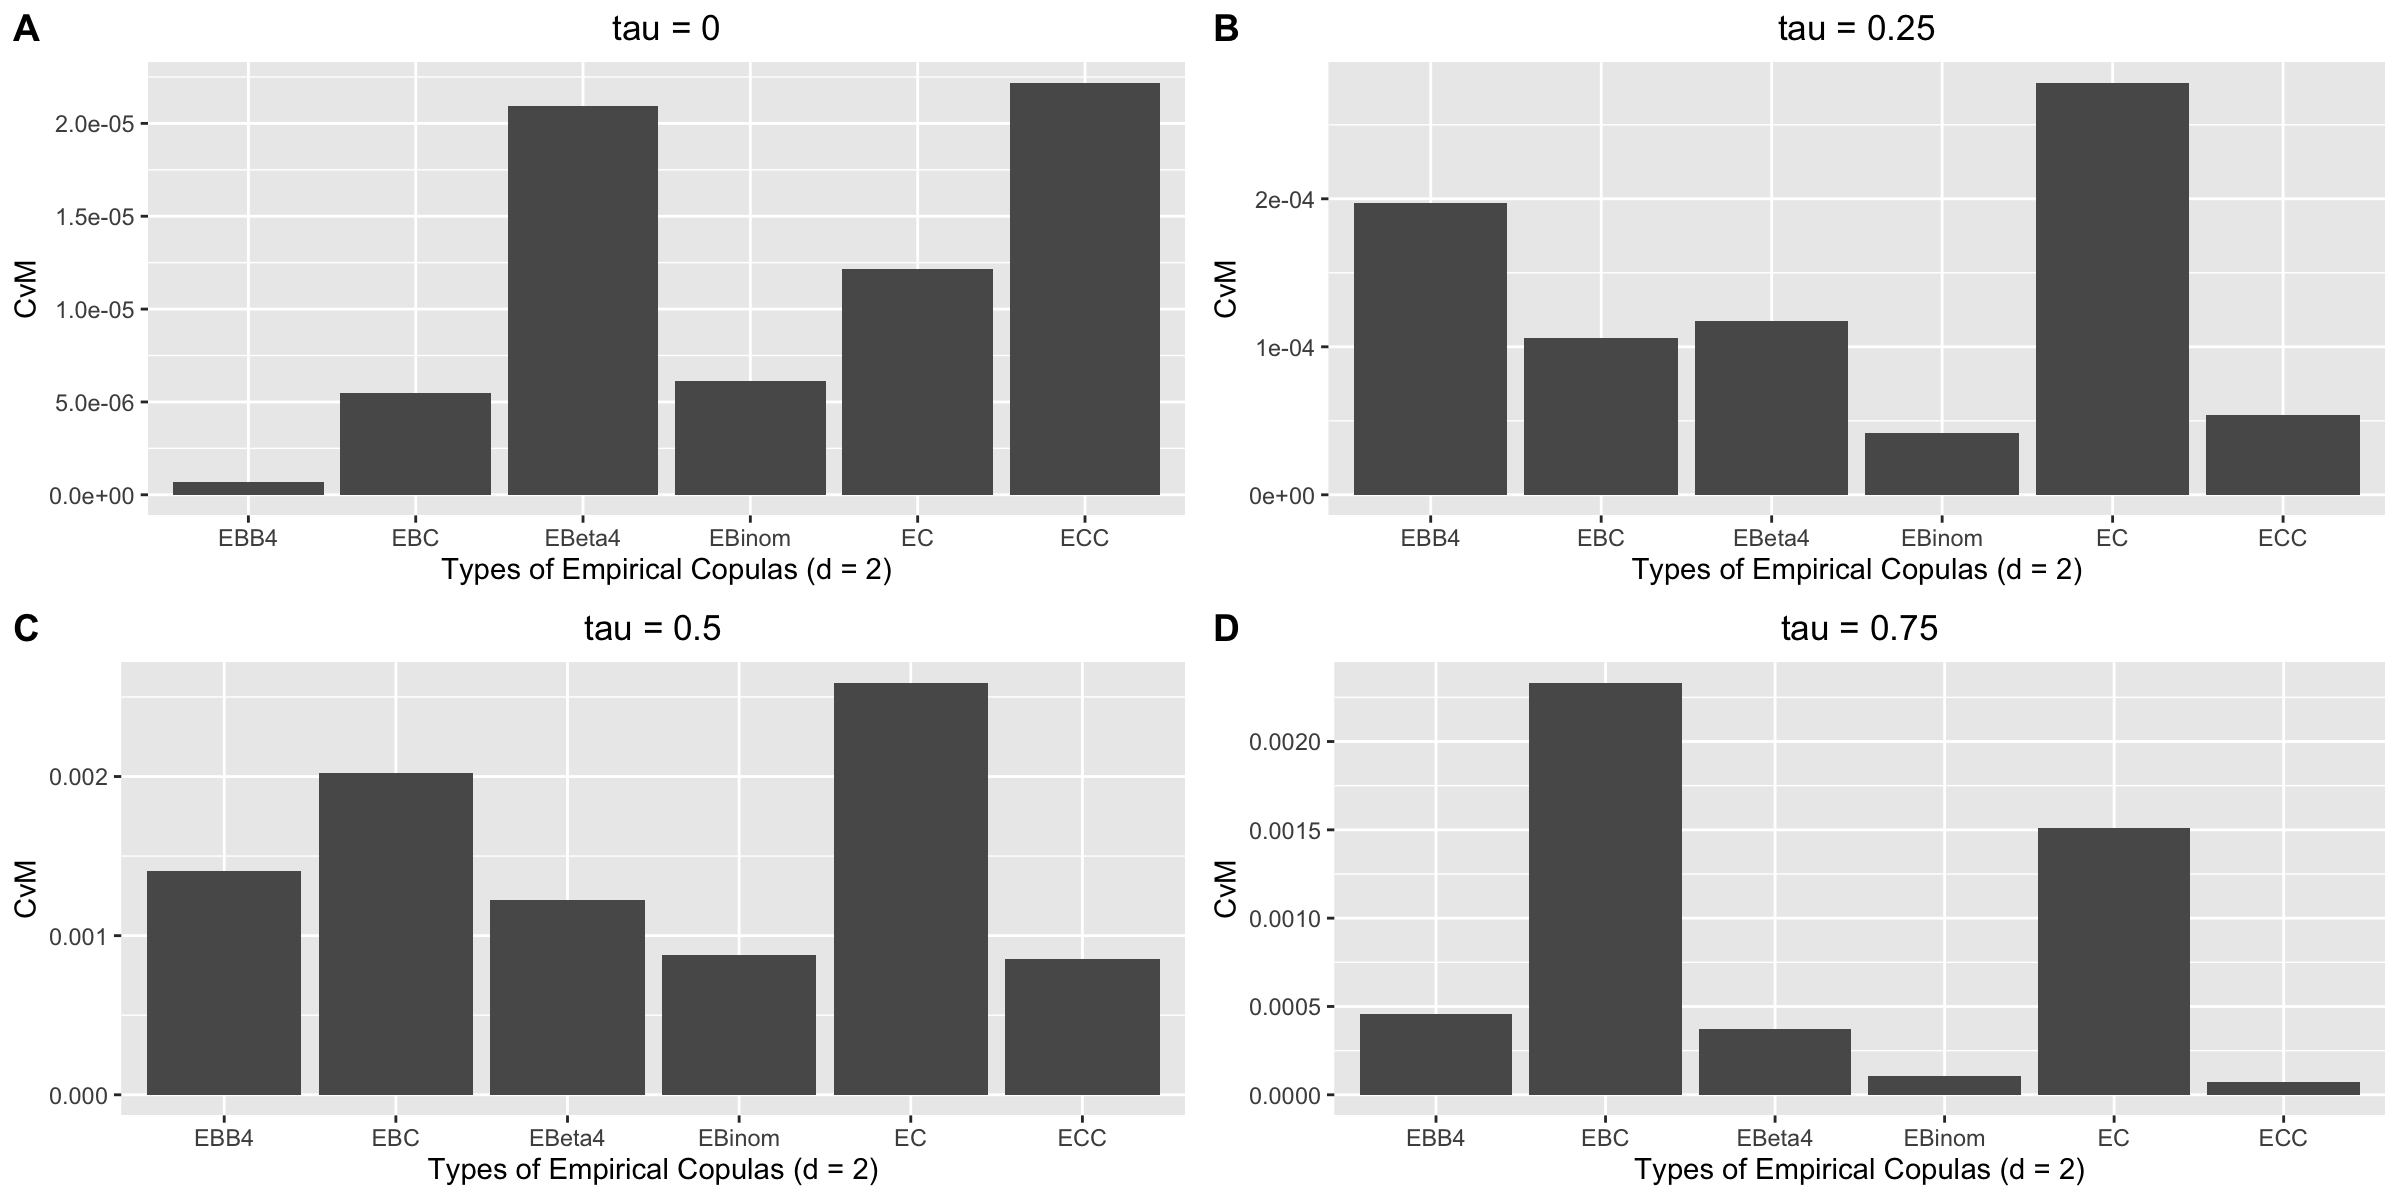
\includegraphics[width=17cm]{ExceedanceCvM/G_2d_s_CvM.png}
\captionof{figure}{Gumbel-Hougaard copula with d = 2}
\end{center}%

\begin{center}
\label{G_3d_s_CvM}
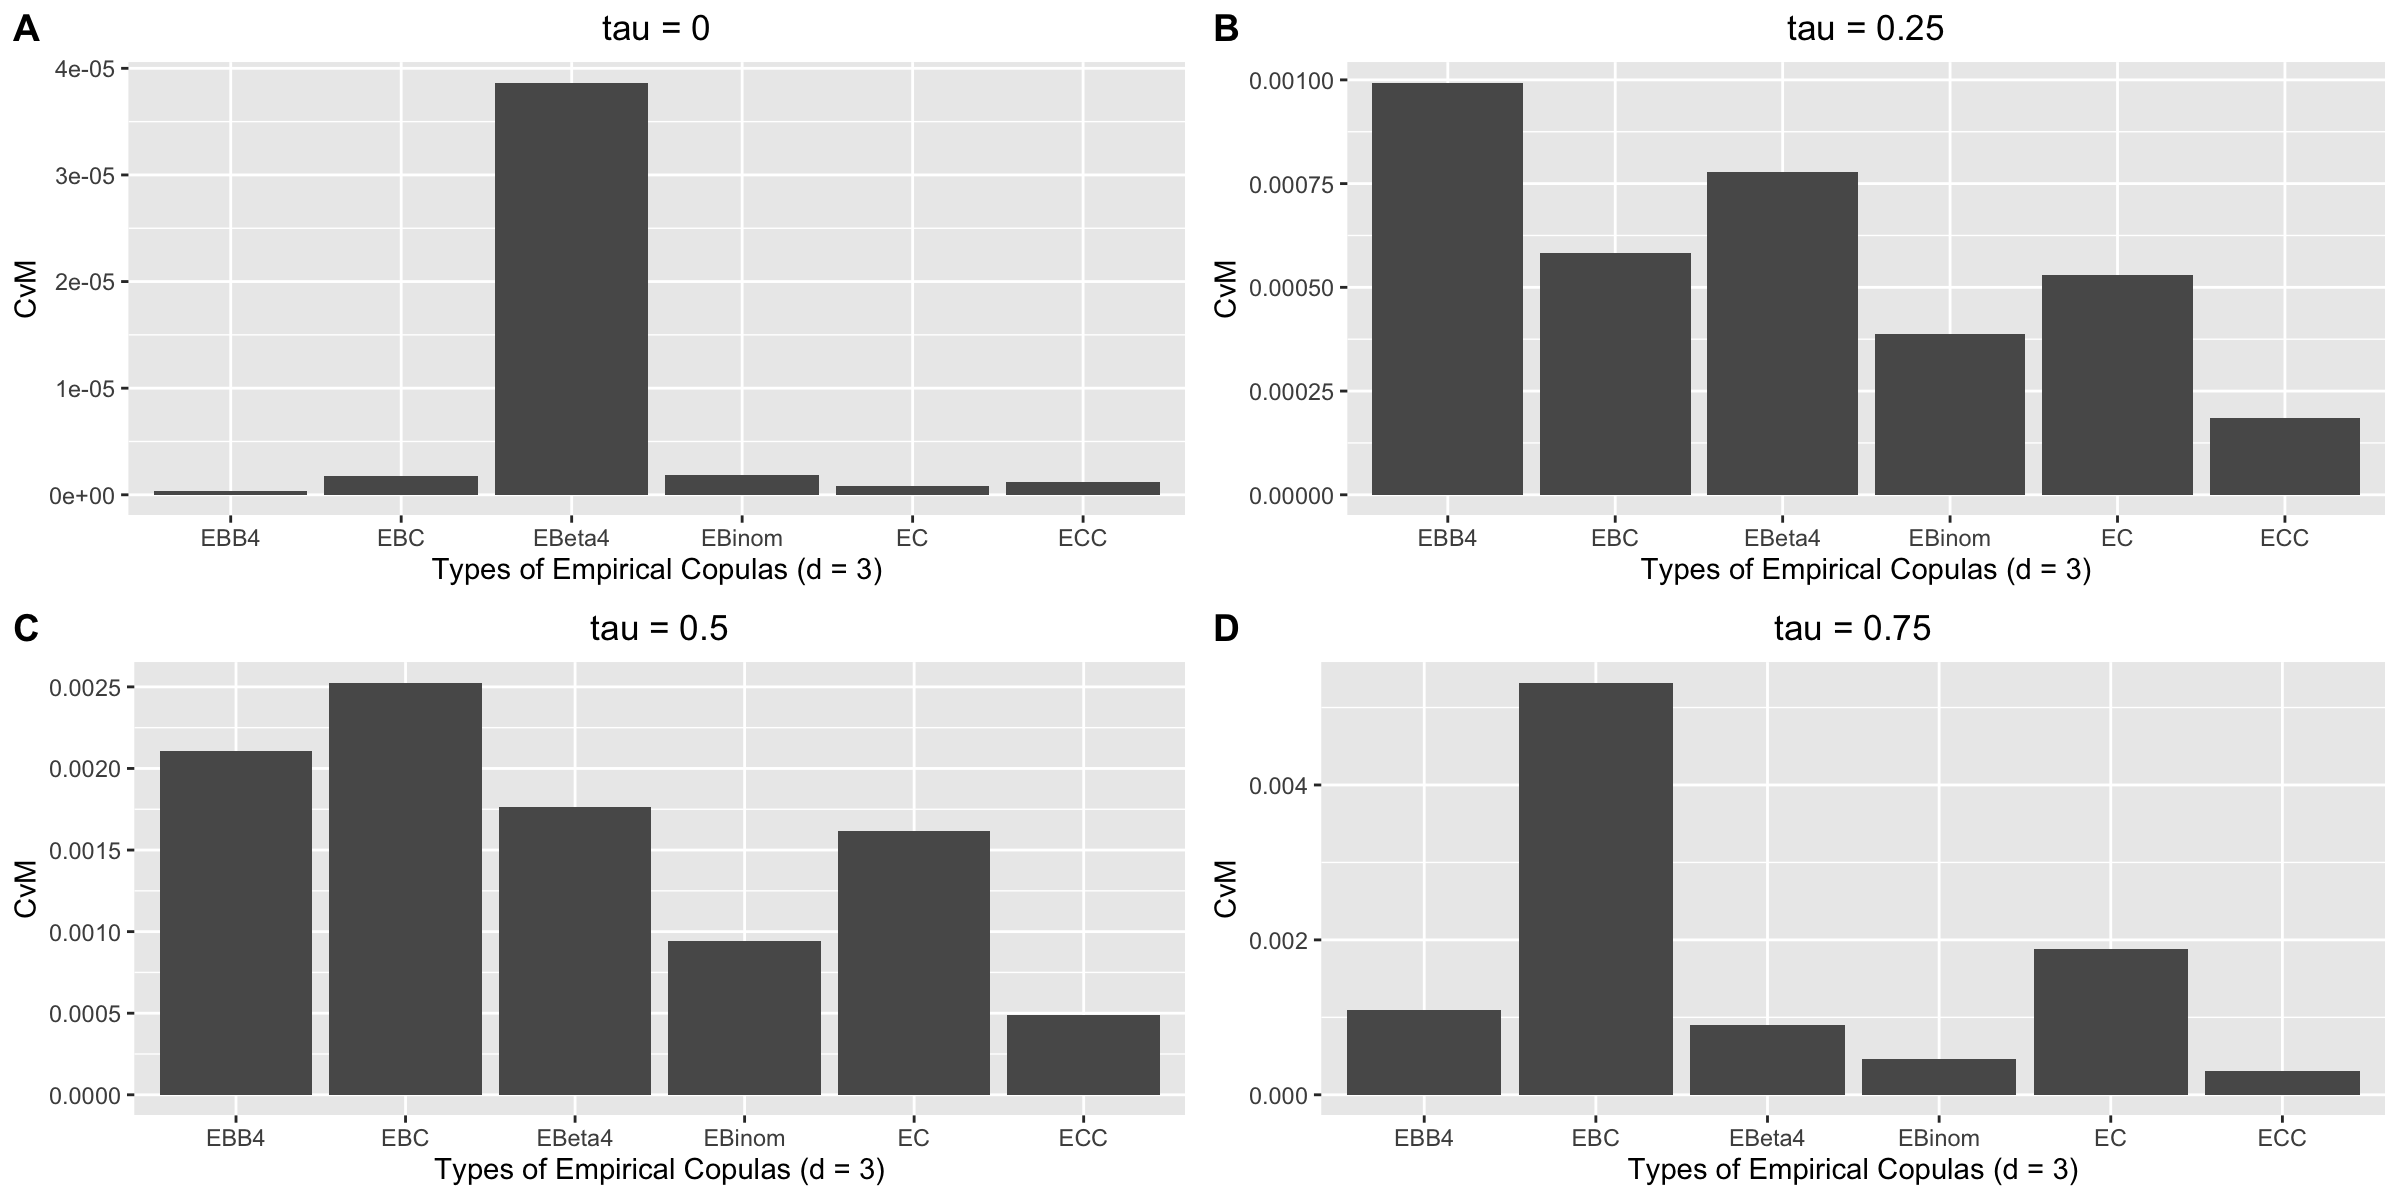
\includegraphics[width=17cm]{ExceedanceCvM/G_3d_s_CvM.png}
\captionof{figure}{Gumbel-Hougaard copula with d = 3}
\end{center}%

\begin{center}
\label{G_4d_s_CvM}
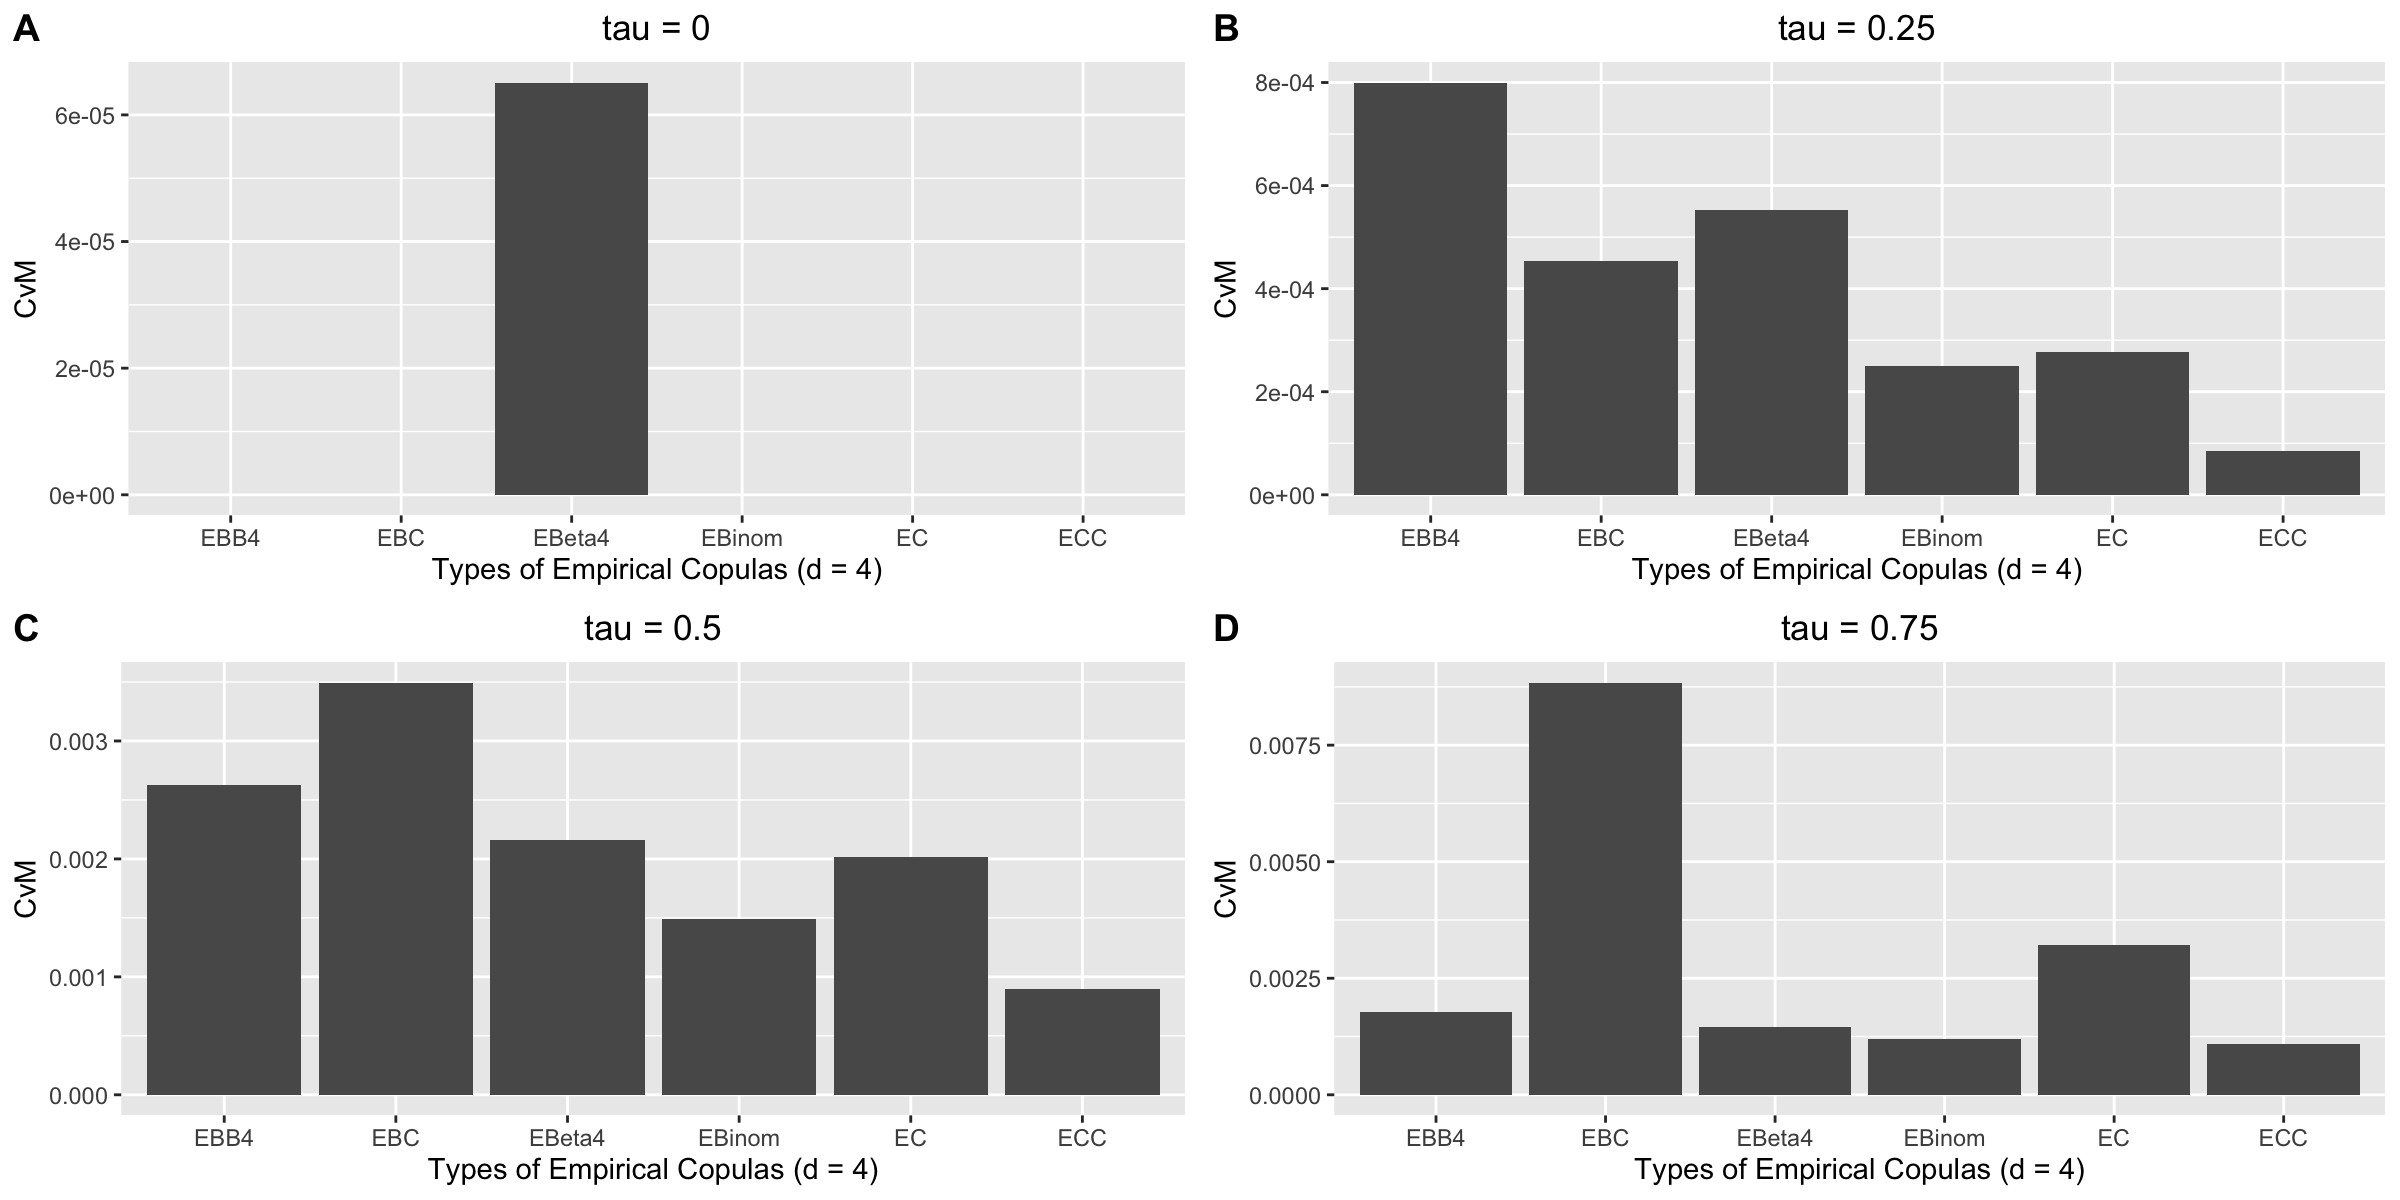
\includegraphics[width=17cm]{ExceedanceCvM/G_4d_s_CvM.png}
\captionof{figure}{Gumbel-Hougaard copula with d = 4}
\end{center}%

\begin{center}
\label{G_5d_s_CvM}
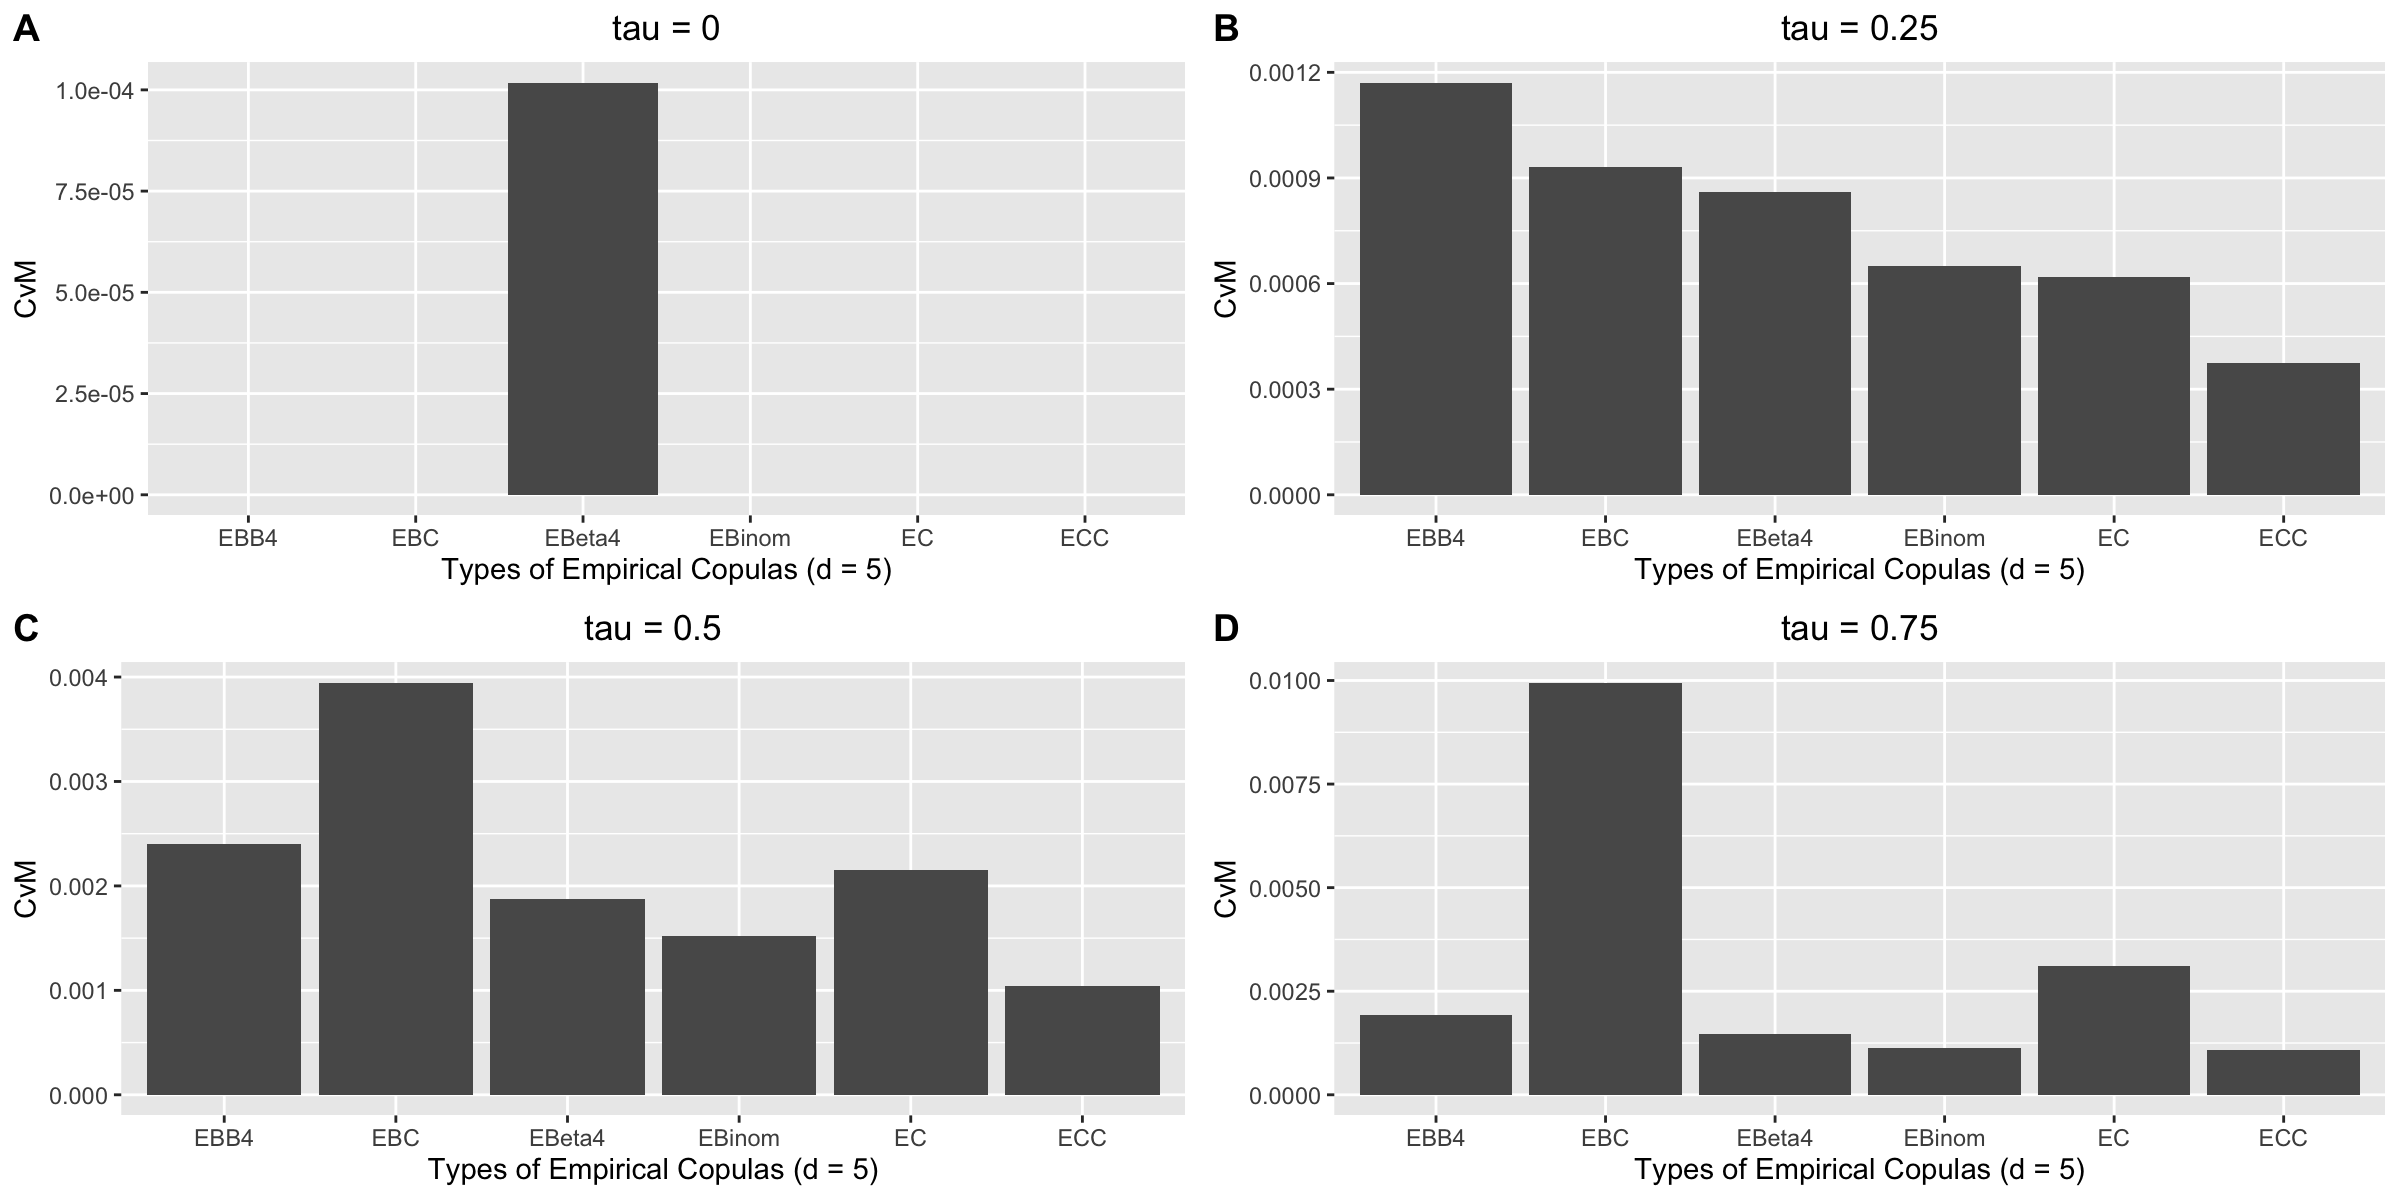
\includegraphics[width=17cm]{ExceedanceCvM/G_5d_s_CvM.png}
\captionof{figure}{Gumbel-Hougaard copula with d = 5}
\end{center}%

\newpage
\subsection{Analysis: Exceedance probabilities}
\vspace{0.5cm}
There are a few conclusions that can be reached by analysed the aforementioned plots. \\

\subsubsection{Lower Kendall's tau values}
\vspace{0.5cm}
It can be observed that there are an overall worse predictive performance at the lower Kendall's Tau (notably negative Kendall's Tau). From intuition, a low Kendall's Tau represents that, for a bivariate case, the independent margins are negatively related (points are concentrated on the top-left or bottom-right corner). Similar intuition holds for high-dimensional cases. Hence, there are little-to-no weight on the lower-tail or upper-tail (i.e. in the bivariate case, bottom-left and top-right corner). In the current analysis, the size of the dataset is relatively small (i.e. $n = 125$). Hence, even when resampling 125 samples from the target true copula, it is unlikely that the sample created will have any weight at the upper tail. Hence, for a smaller tau, most copulas (except beta-survival margins smoothed empirical copula) vastly underestimates the upper tail. It is noted that some graphs show a systematic overestimation with respect to the true copula, which is intuitive; as the probability of having samples at the extreme tail (for low Kendall's Tau values) are low, sampling differences might bring the estimated copula to underestimate or overestimate the true copula.\\
\vspace{0.5cm}
It is notable that the smoothed EBC-adapted empirical copula with beta-binomial survival margins seems to best estimate the true-copula at lower values of Kendall's tau, compared to the other two types of smoothed empirical copula. \\
\vspace{0.5cm}
To more accurately estimate the true-copula by using the class of empirical copulas, a larger $n$ is needed, as the class of empirical copula asymptotically converges to the true copula for large $n$. However, this becomes prohibitive when available data is not sufficient. 

\pagebreak
\subsubsection{Erratic behaviour from smoothed EBC-adapted empirical copula with beta survival margins}

It can be seen from the plots that the smoothed EBC-adapted empirical copula with beta survival margins have extremely volatile behaviour at the tail. It is noted that it is uncertain why the "survival function" exhibits a non-monotone pattern, as it is likely to be caused by rounding errors at the edge, as the order of the exceedance probabilities are from negative 5 to 10. \\
\vspace{0.5cm}
However, it is still interesting to understand the reason why, unlike the other types of empirical copulas, there appears to be a hump near $u = 0.99$.\\
\vspace{0.5cm}
Recall that the smoothed EBC-adapted empirical copula with beta survival margins is defined as follows:
\begin{align*}
C_{n}^{v}(\textbf{u}) &= \frac{1}{n} \sum\limits_{i = 1}^{n} C_{n}^{\beta} \left[\Bar{F}_{u_{1}}^{\textbf{X}}\left(\frac{R_{i,1} - 0.5}{n}\right), \dots, \Bar{F}_{u_{d}}^{\textbf{X}}\left(\frac{R_{i,d} - 0.5}{n}\right) \right]
\end{align*}
where $\Bar{F}_{u_{j}}^{\textbf{X}}$ is beta distributed. The survival function corresponding to this type of smoothed empirical copula is computed as follows:
\begin{align*}
\Bar{H}^{v}_{n}(\textbf{u}) = \Bar{C}^{v}_{n}(\textbf{1 -- u}) = \sum\limits_{J \subseteq \{1, \dots, d \} }(-1)^{|J|} C^{v}_{n} \left( u_{1}^{\mathds{1}(1\in J)}, \dots, u_{d}^{\mathds{1}(d\in J)} \right), \: \: \textbf{u} \in [0,1]^{d}
\end{align*}
Hence we can see the main determinant of the size of the survival function is entirely dependent on the smoothed EBC-adapted empirical copula with dimensions $d \in \{1, \dots, d\}$. Note that the beta distribution defined above is distributed as follows (proof is by algebraic manipulation, and can be found in \cite{KojadinovicYi2024Smooth}):
\begin{align*}
\alpha &= \frac{n - \rho}{\rho} \times u_{j}, \: j \in \{1, \dots, d\} \\
\beta &= \frac{n - \rho}{\rho} \times (1 - u_{j}), \: j \in \{1, \dots, d\}
\end{align*}
In this simulation, $n = 125$ and $\rho = 4$, and $u_{j} \in \{0.95, \dots, 1\}$. The resulting $\alpha$ can be calculated as: $\alpha \in [28.7375, 30.25]$, and the resulting $\beta$ can be calculated as: $\beta \in [0, 1.5125]$. Hence, this is equivalent (componentwise), in evaluating the probability of a beta distribution with $\alpha \in [28.7375, 30.25]$ and $\beta \in [0, 1.5125]$ larger than $\frac{R_{i,j} - 0.5}{n} \in (0,1)$. As the resulting $\alpha$ is extremely large and resulting $\beta$ is extremely small, this results in a extremely heavy-right-tailed beta distribution. Substituting into the smoothed empirical EBC-adapted empirical copula, it will result in a very abnormally large copula $C^{v}_{n} \left( u_{1}^{\mathds{1}(1\in J)}, \dots, u_{d}^{\mathds{1}(d\in J)} \right)$, and hence a peak in the exceedance probability. As the appearance of a "up-tail" data point is rare during resampling procedures, this sudden peak in the exceedance probability (in one data row) will skew the average exceedance probability. In further analysis, it is ideal to increase the sample size to see if this observations is retained.\\
\vspace{0.5cm}
With the following revelation, the smoothed EBC-adapted empirical copula with beta survival margins are very suitable (under a larger sample size n) to model extremal events (such as joint default scenarios).

\subsubsection{Systemic underestimation of the upper-tail at positive Kendall's tau}

\newpage
\subsection{Plots: $\textbf{u}$ (evaluation points) vs cumulative probabilities}
\vspace{0.5cm}
We then plot the (lower-tailed) evaluation points against the cumulative probabilities for each empirical copula. The evaluation points are on the x-axis and the cumulative probabilities are on the y-axis.

\begin{center}
\label{t4_2d_c}
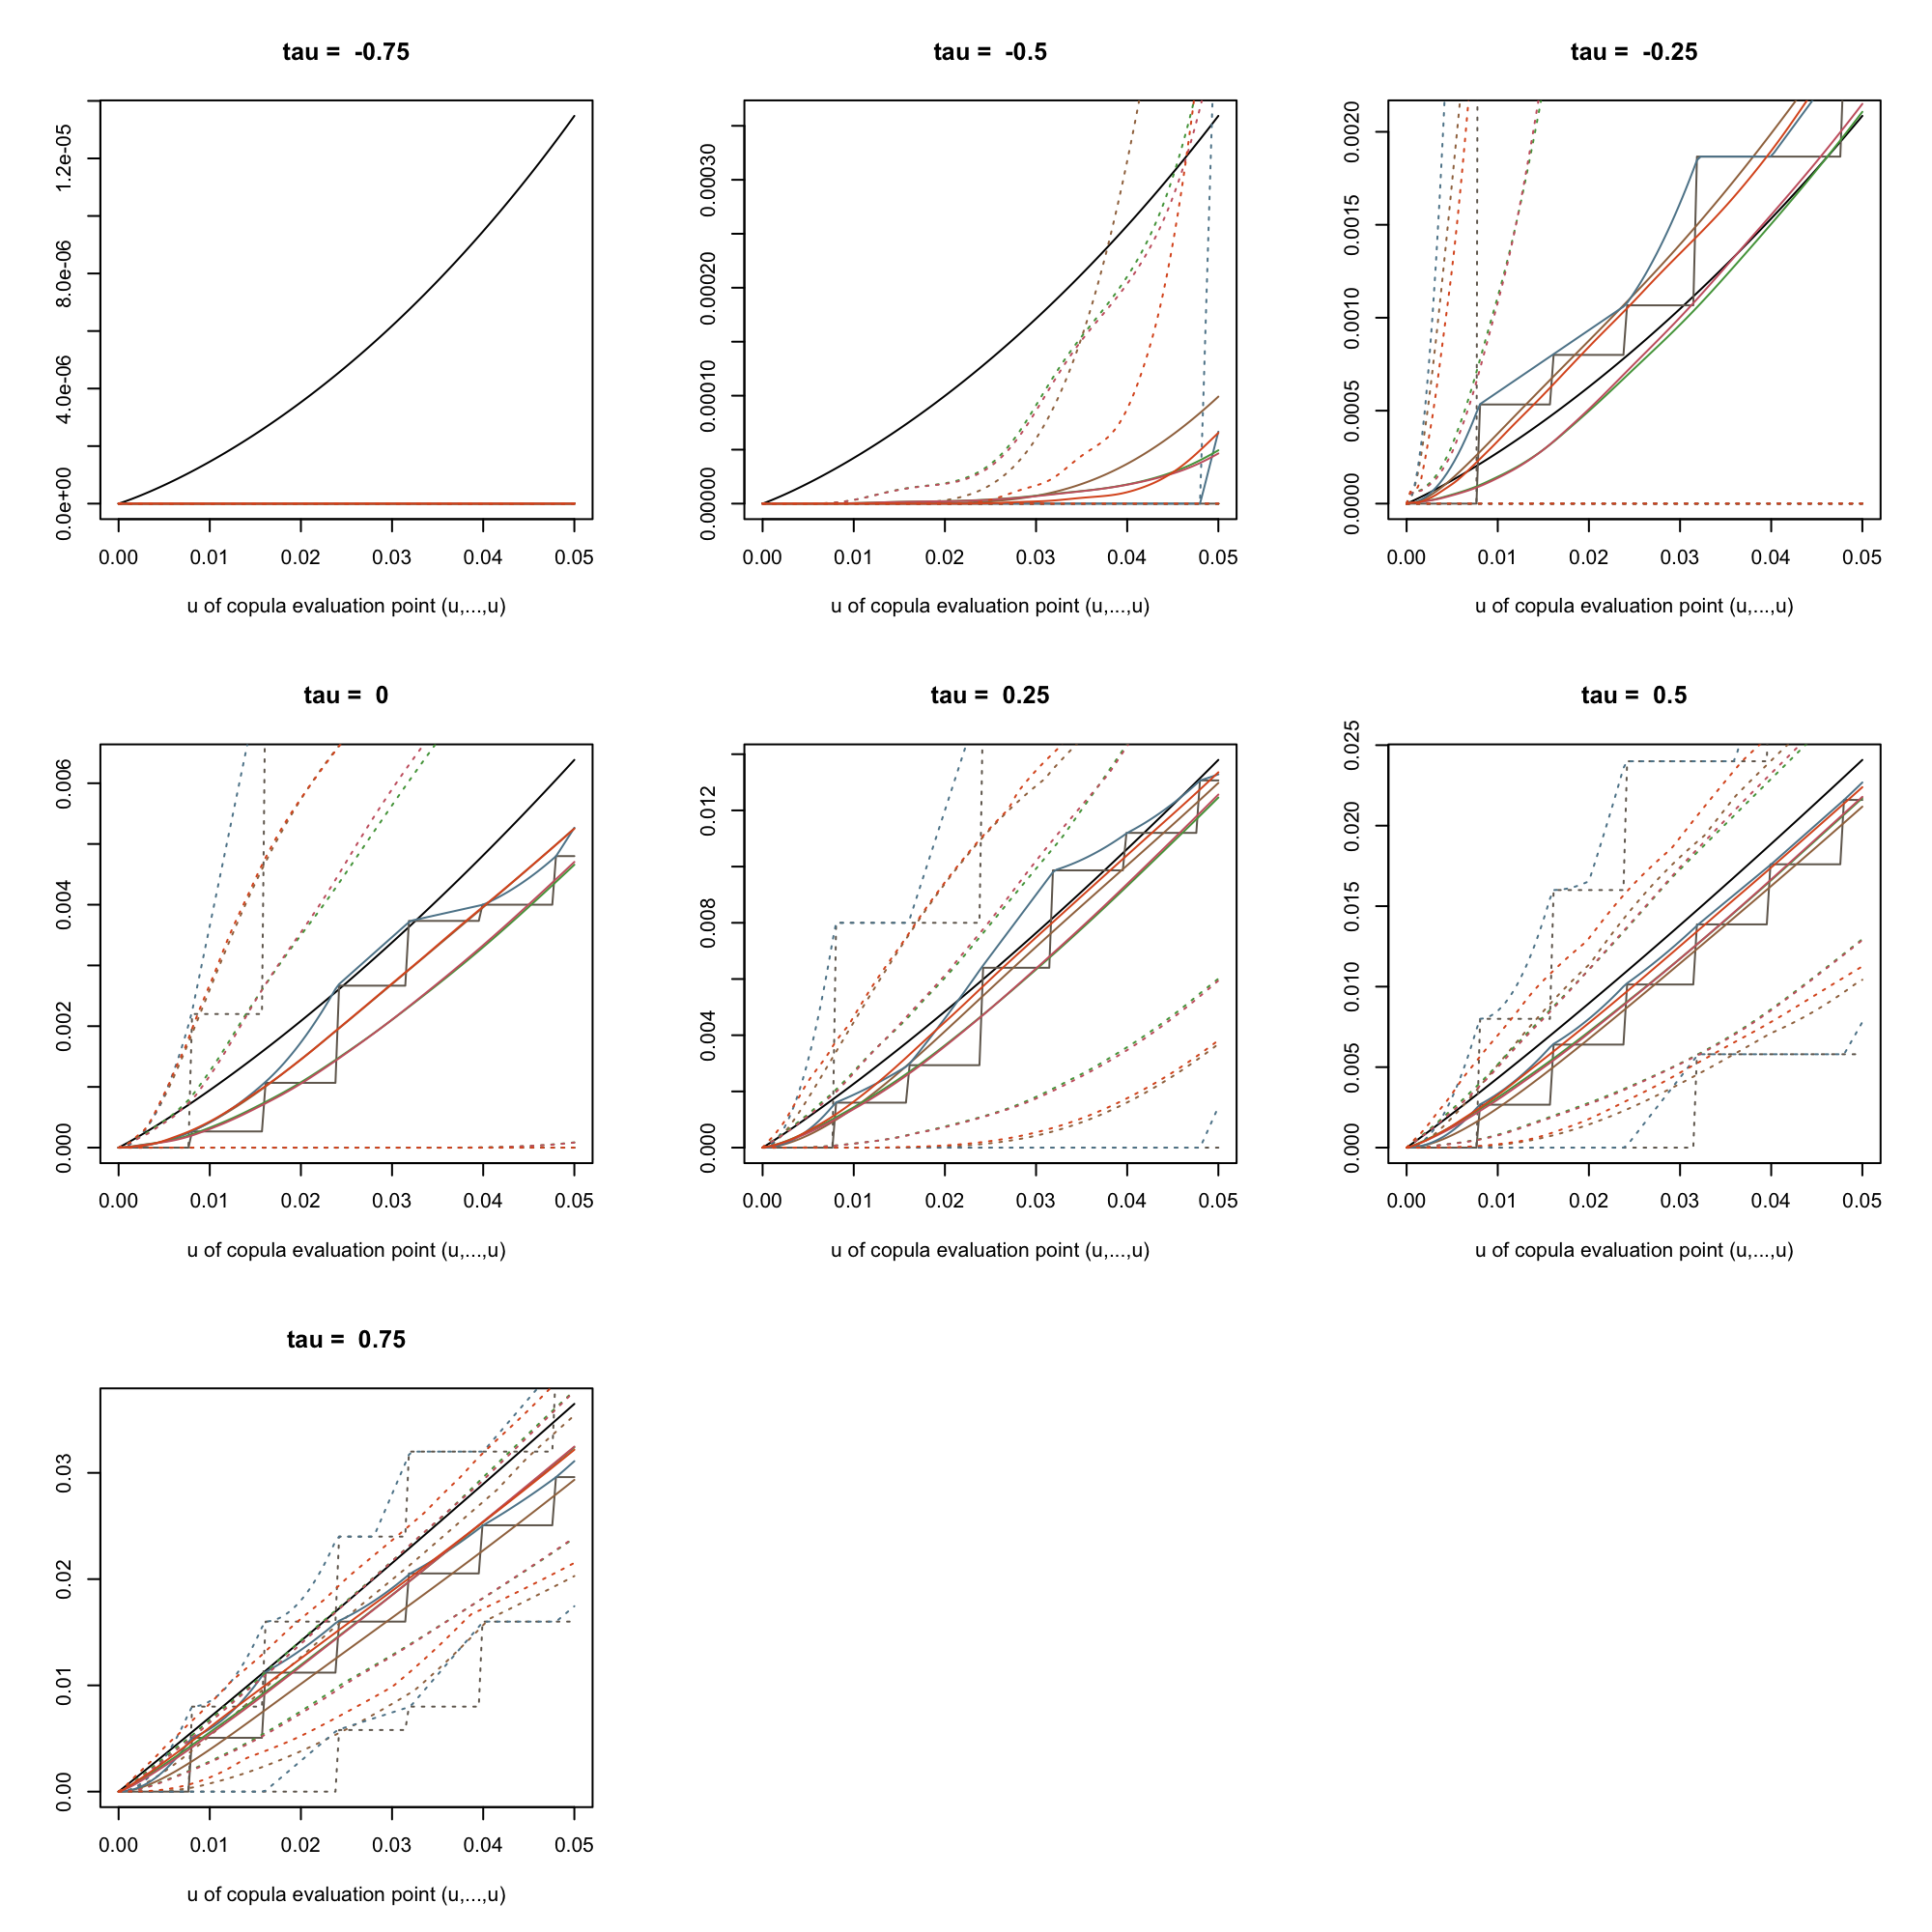
\includegraphics[width=17cm]{CumulativeProb/t4_2d_c.png}
\captionof{figure}{Student-t copula with d = 2}
\end{center}%

\begin{center}
\label{N_2d_c}
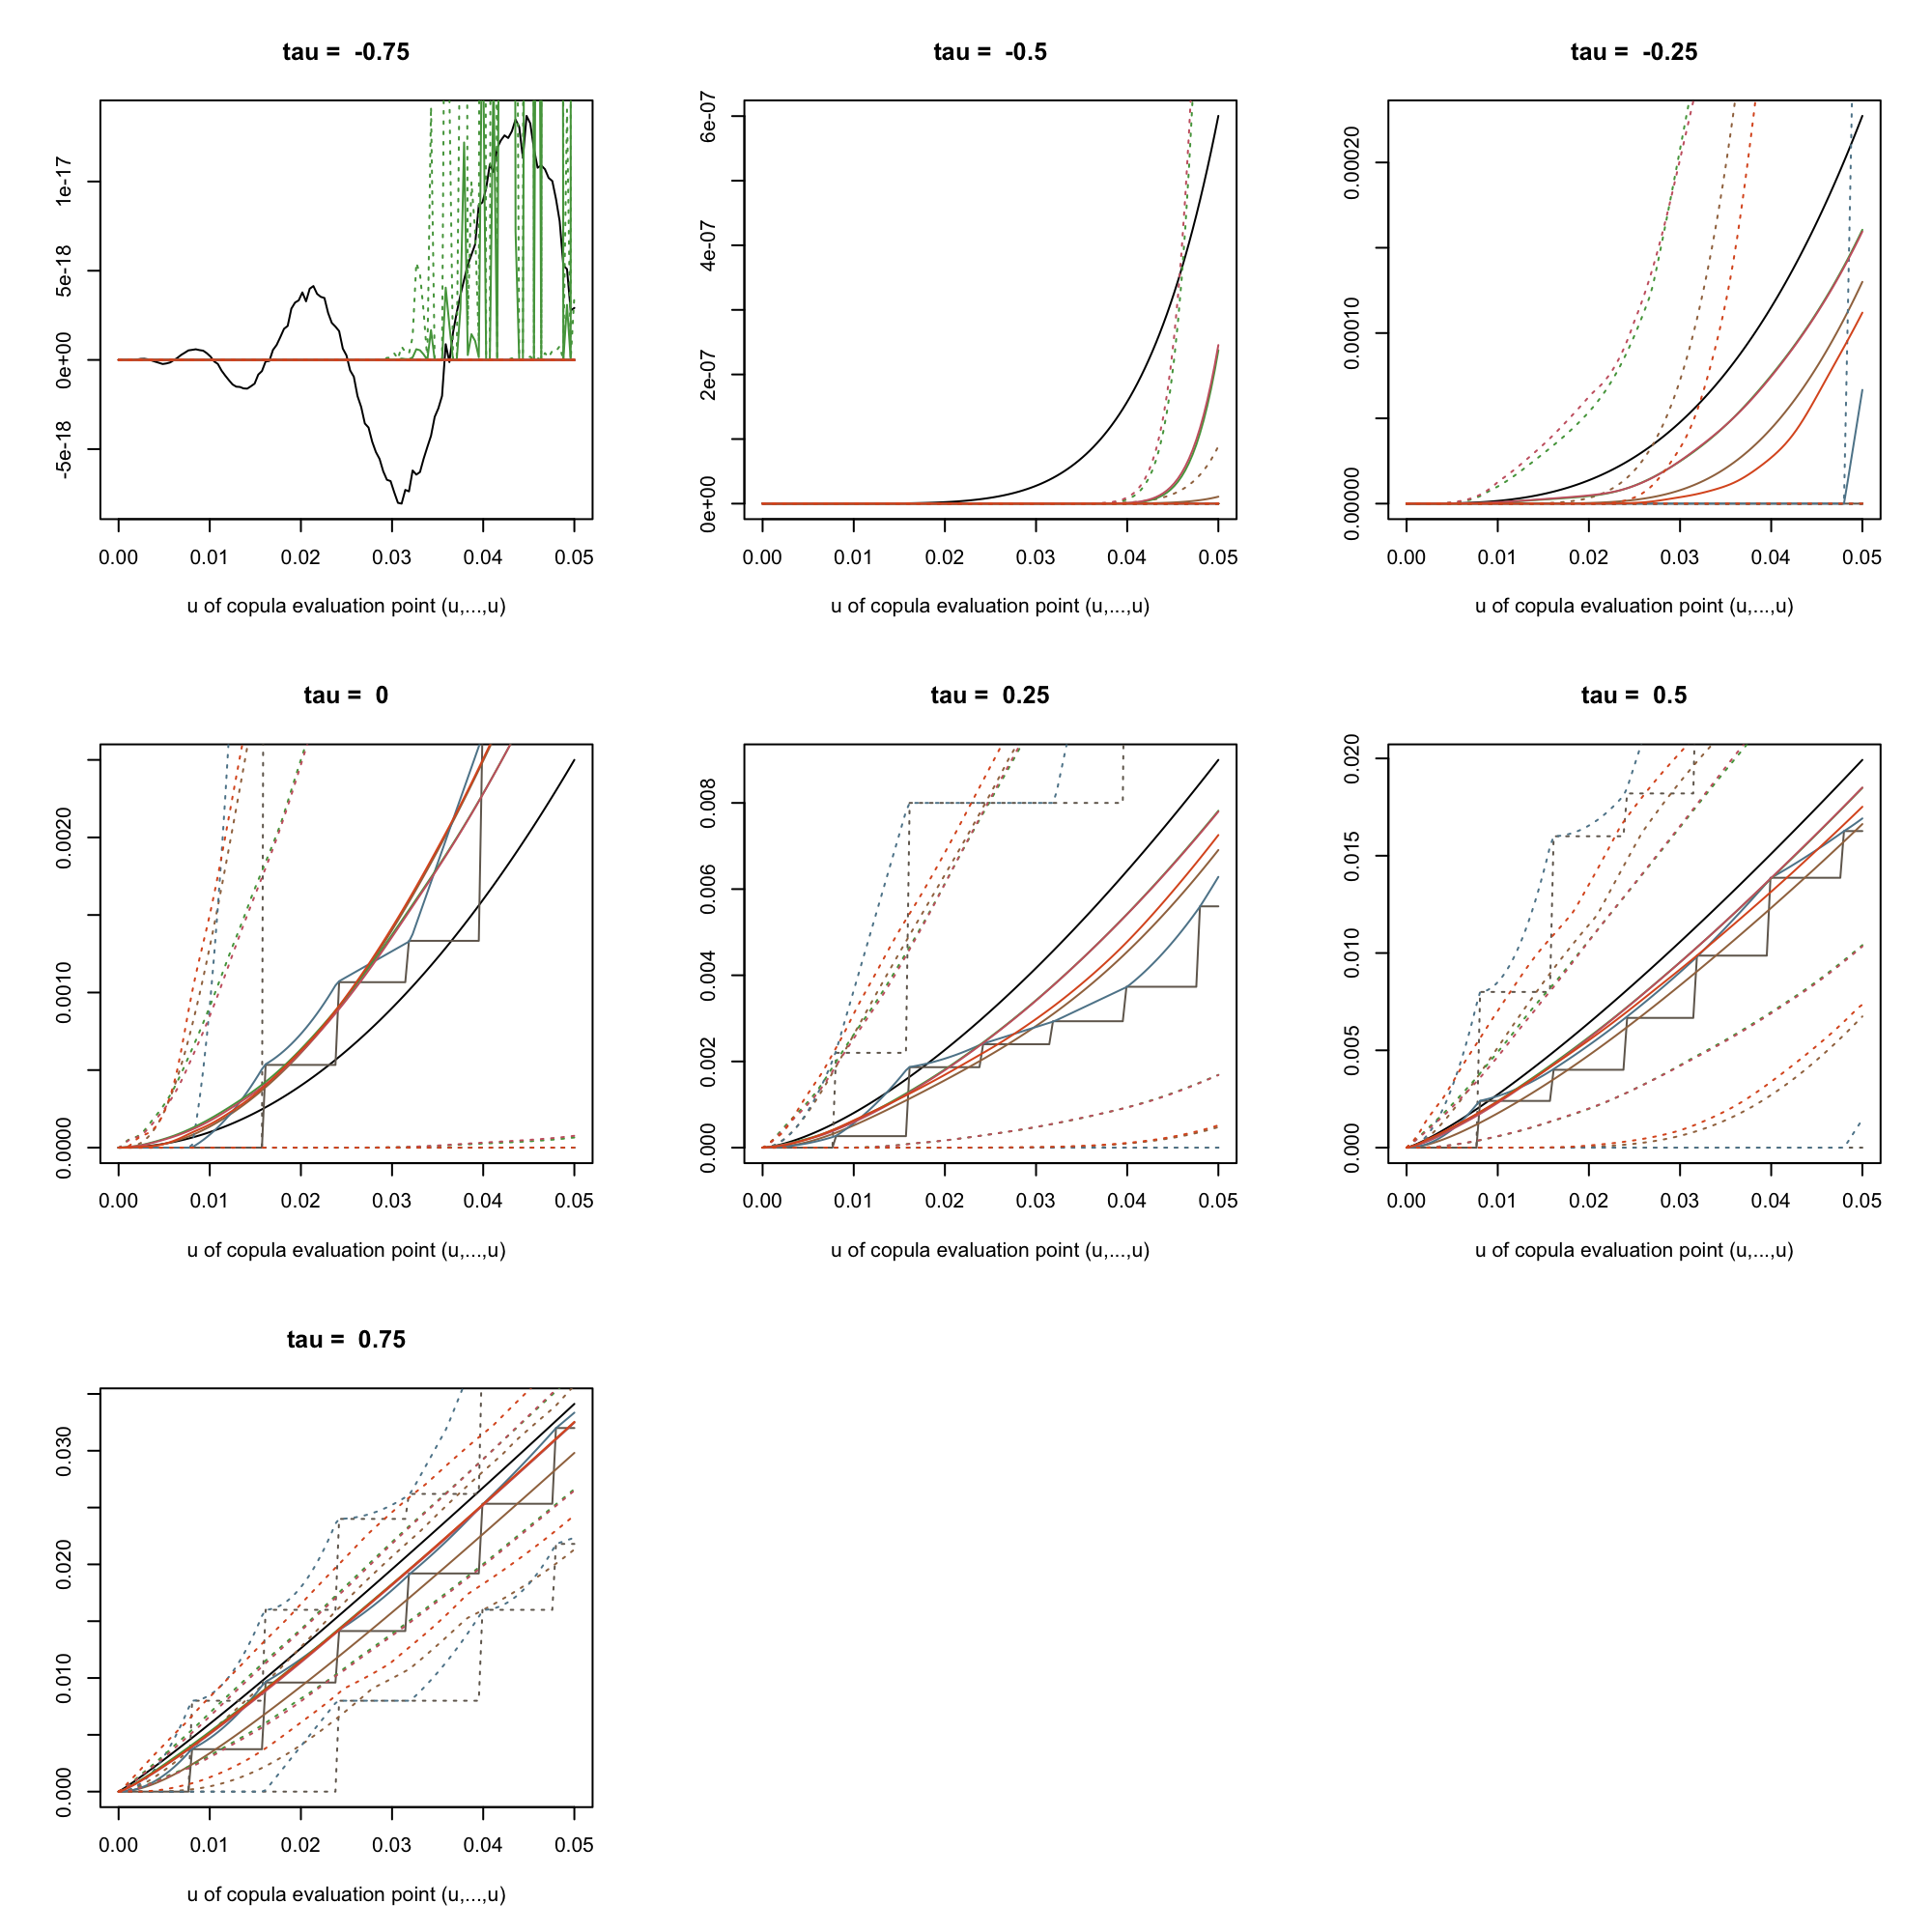
\includegraphics[width=17cm]{CumulativeProb/N_2d_c.png}
\captionof{figure}{Gaussian copula with d = 2}
\end{center}%

\begin{center}
\label{C_2d_c}
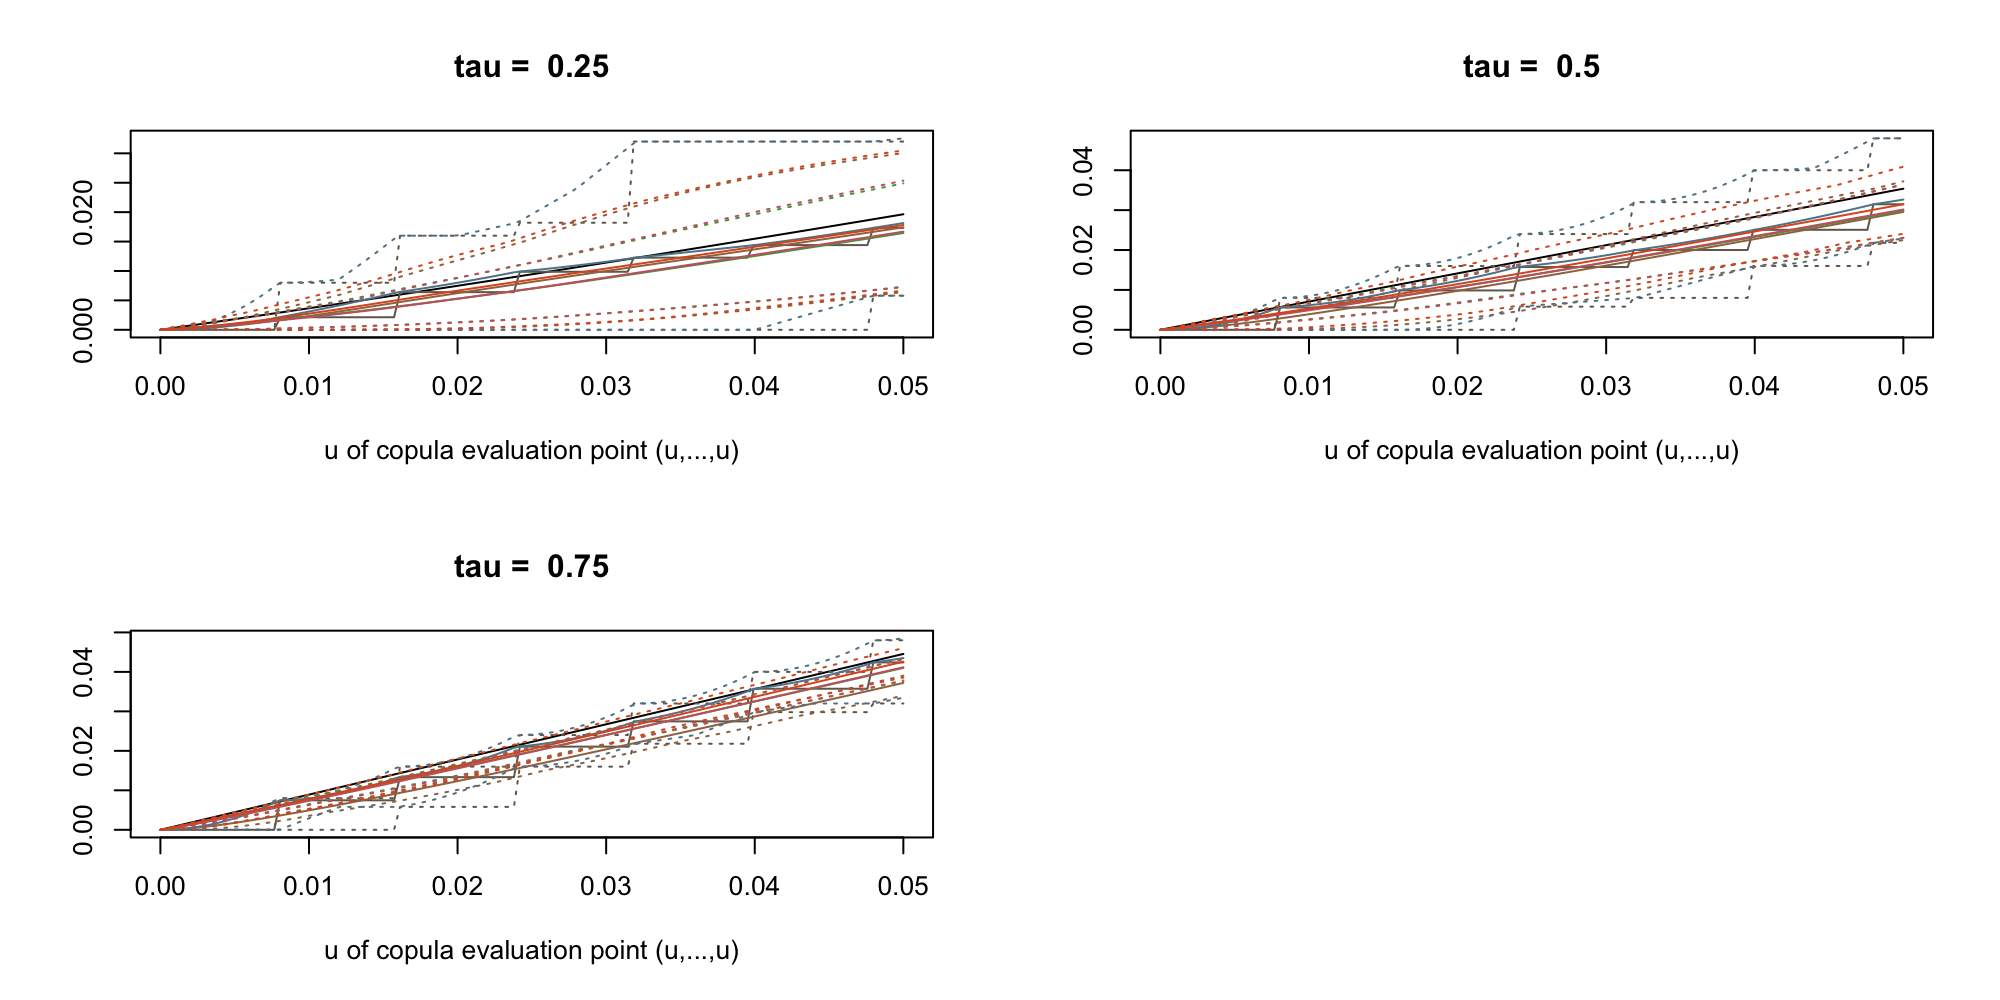
\includegraphics[width=17cm]{CumulativeProb/C_2d_c.png}
\captionof{figure}{Clayton copula with d = 2}
\end{center}%

\begin{center}
\label{C_3d_c}
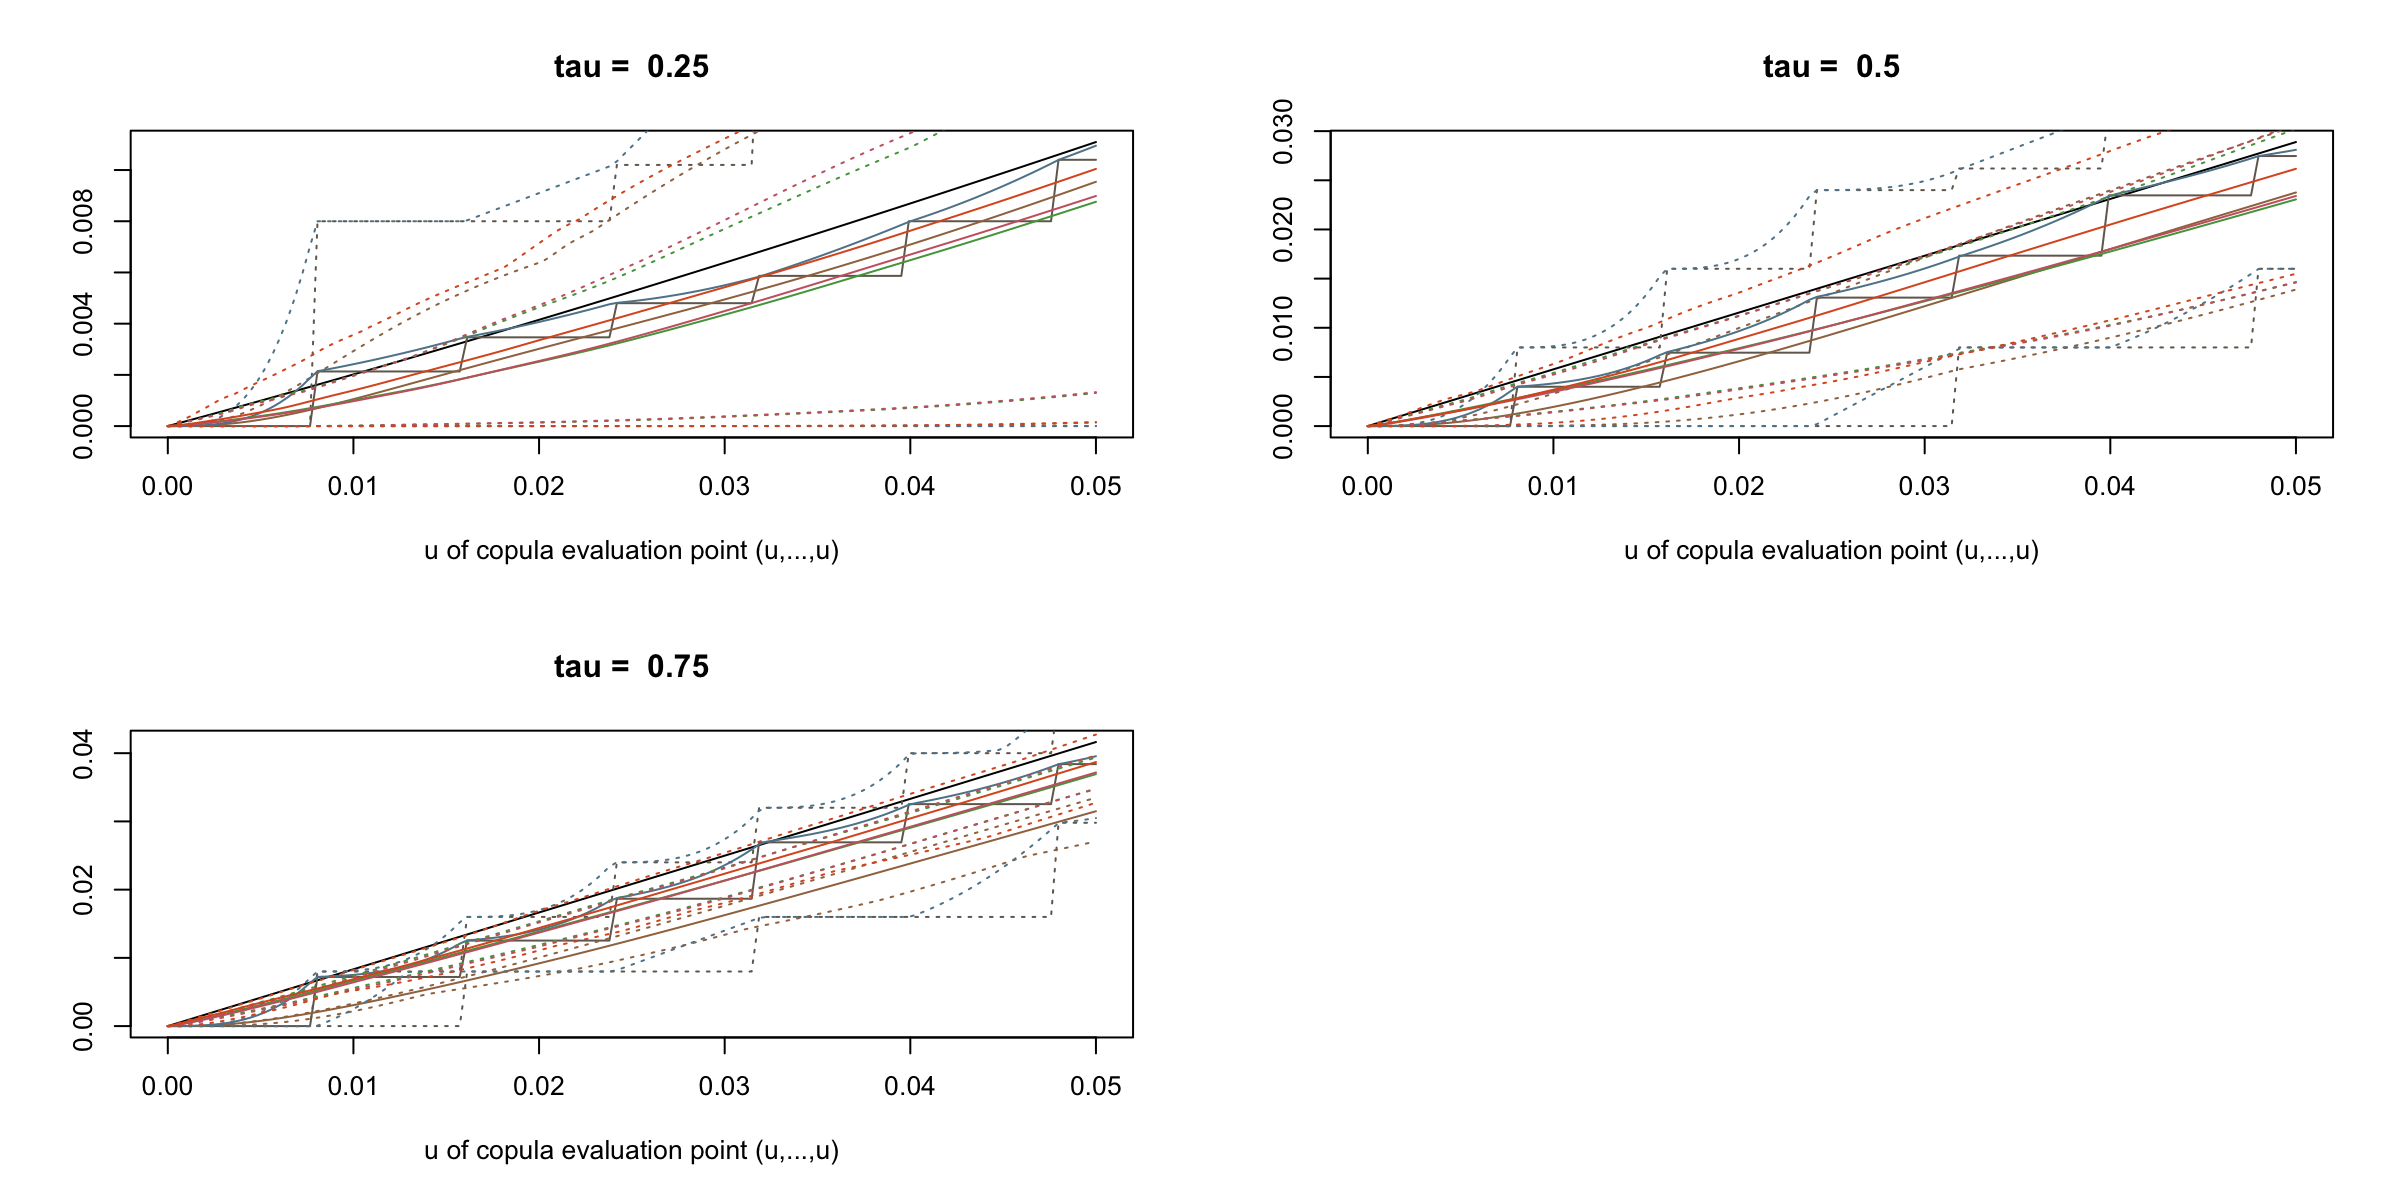
\includegraphics[width=17cm]{CumulativeProb/C_3d_c.png}
\captionof{figure}{Clayton copula with d = 3}
\end{center}%

\begin{center}
\label{C_4d_c}
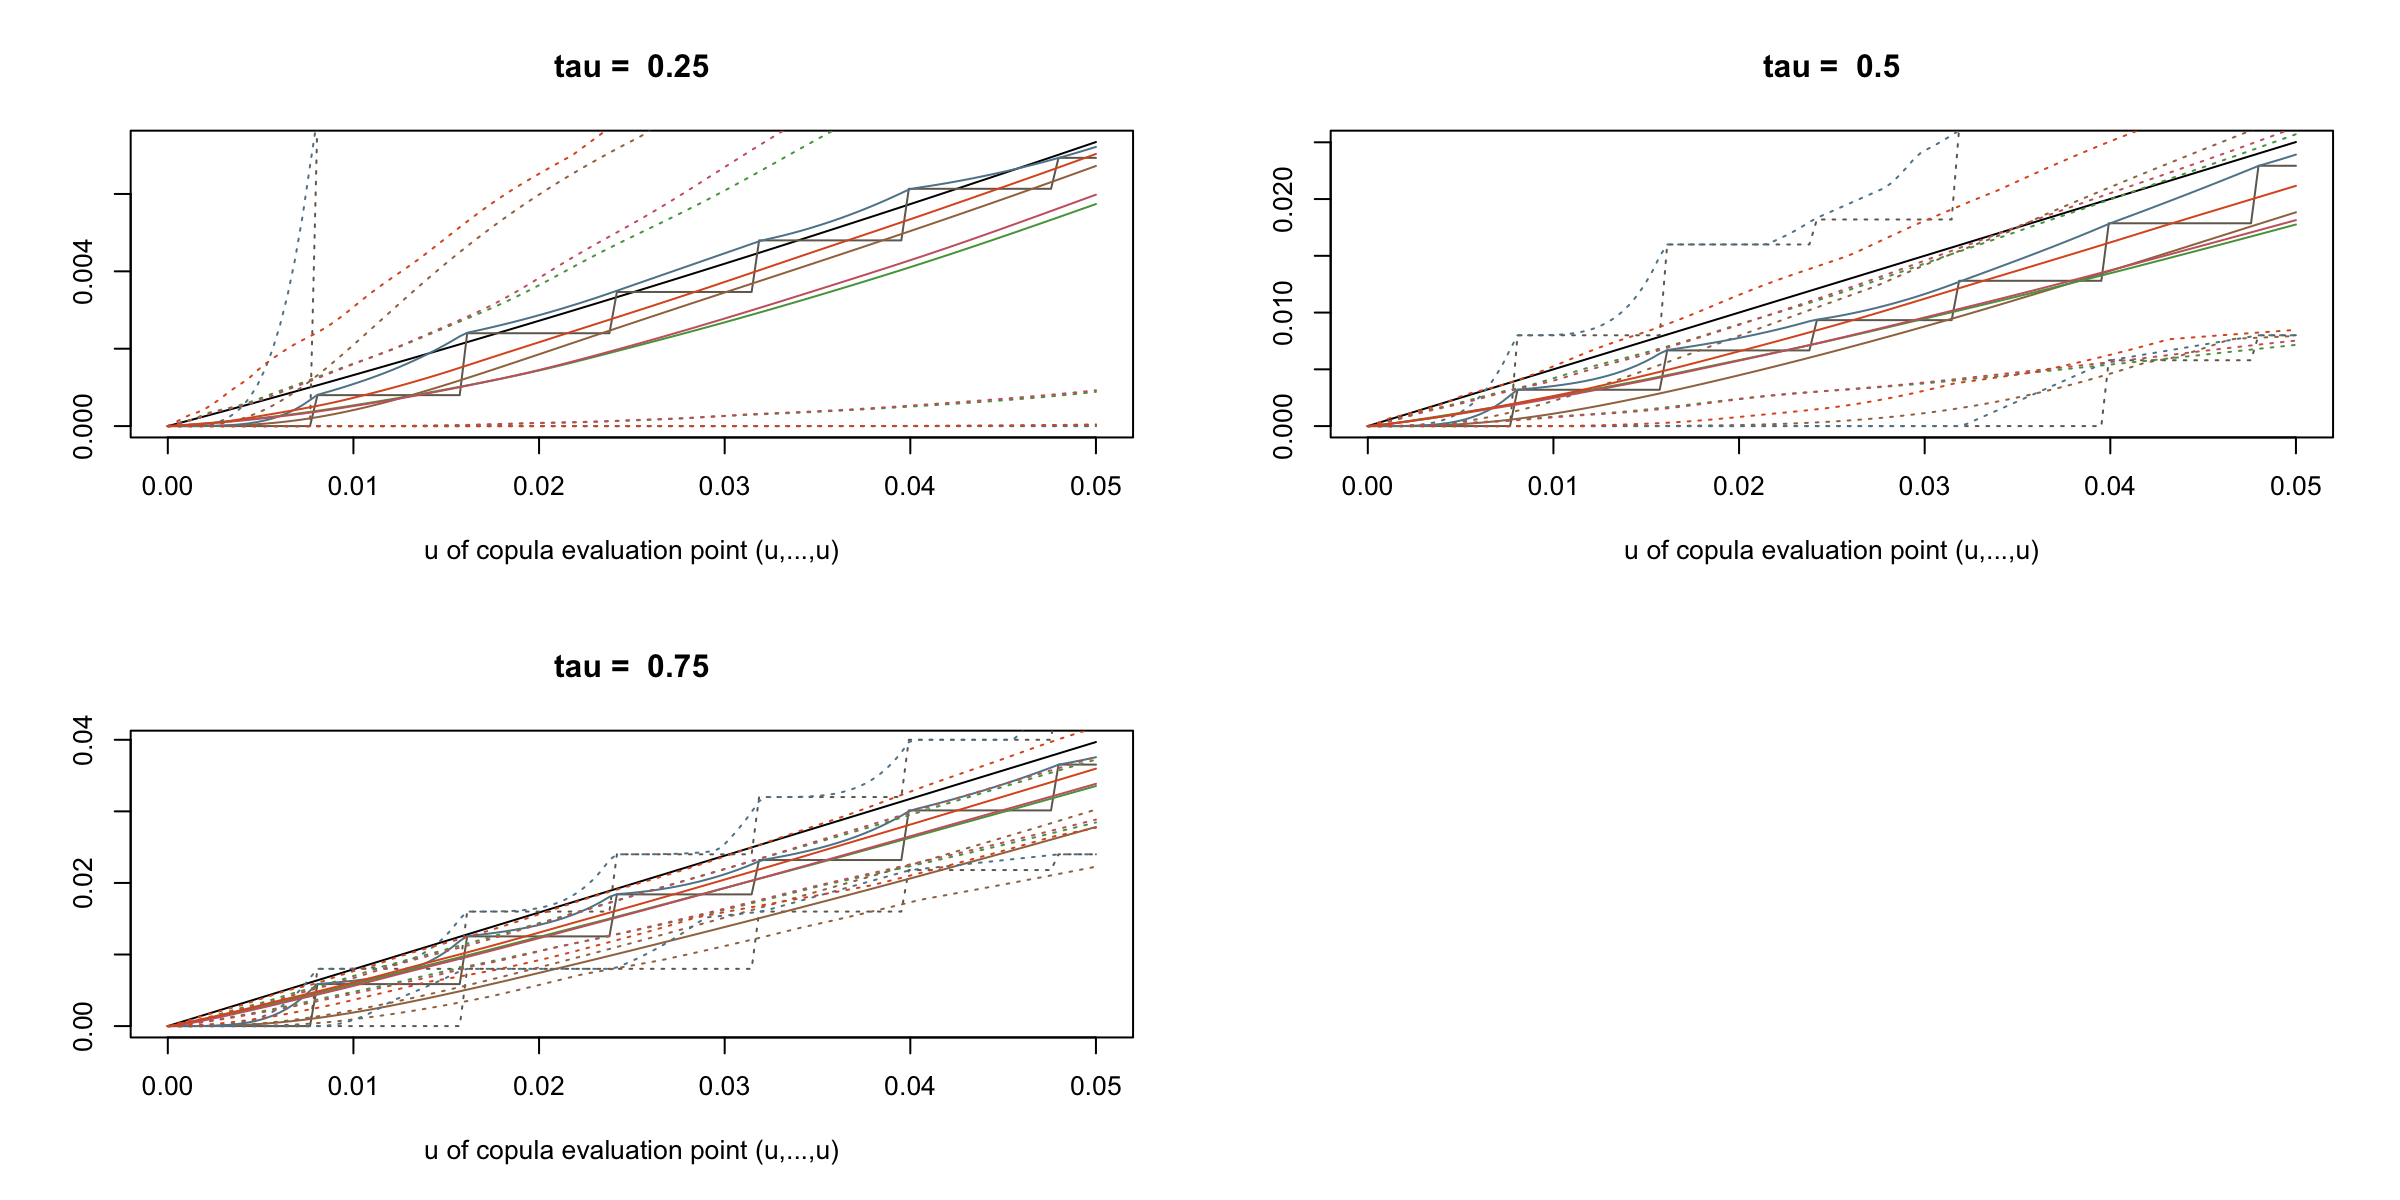
\includegraphics[width=17cm]{CumulativeProb/C_4d_c.png}
\captionof{figure}{Clayton copula with d = 4}
\end{center}%

\begin{center}
\label{C_5d_c}
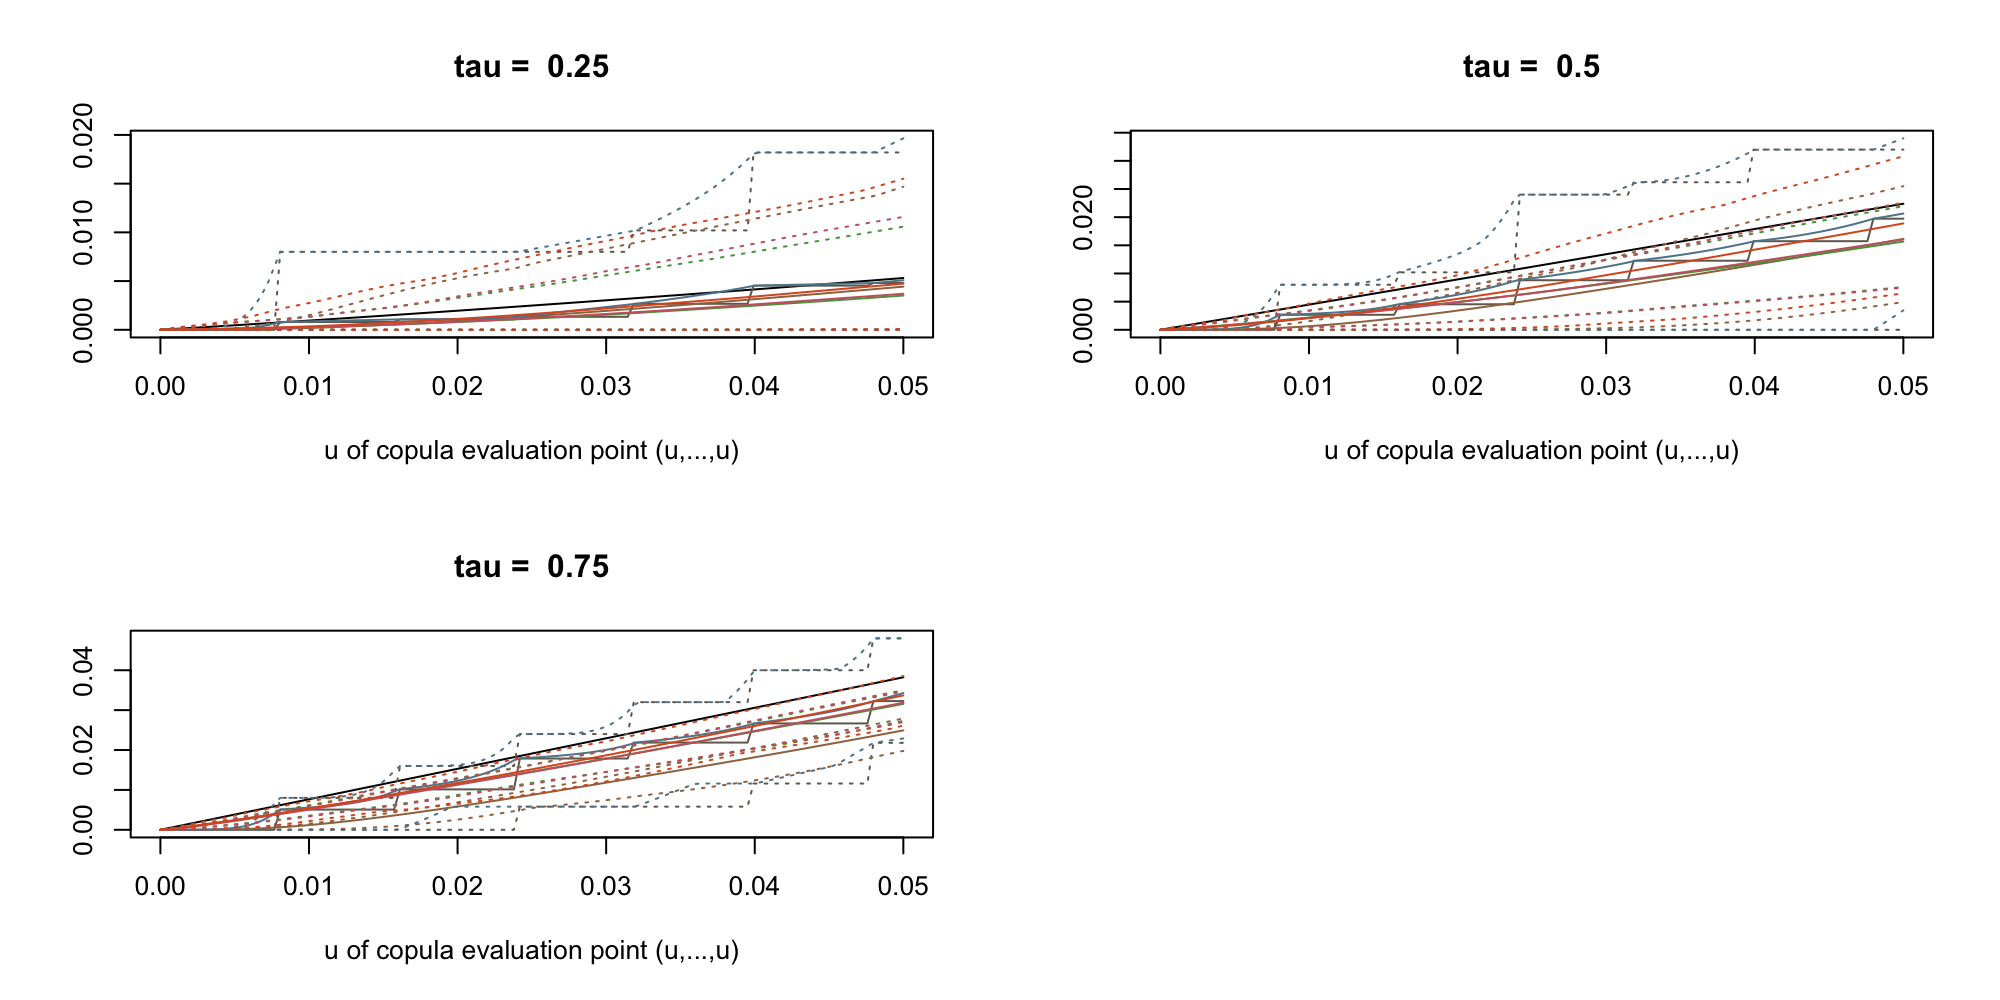
\includegraphics[width=17cm]{CumulativeProb/C_5d_c.png}
\captionof{figure}{Clayton copula with d = 5}
\end{center}%


\newpage
\subsection{CvM: Cumulative probabilities}
To better understand the proximity of the cumulative probabilities for the class of empirical copula, with respect to the true copula, we then compute the Cramer-von-Mises statistics for all combinations of empirical copulas, Kendall's Tau and dimensions.

\begin{center}
\label{t4_2d_c_CvM}
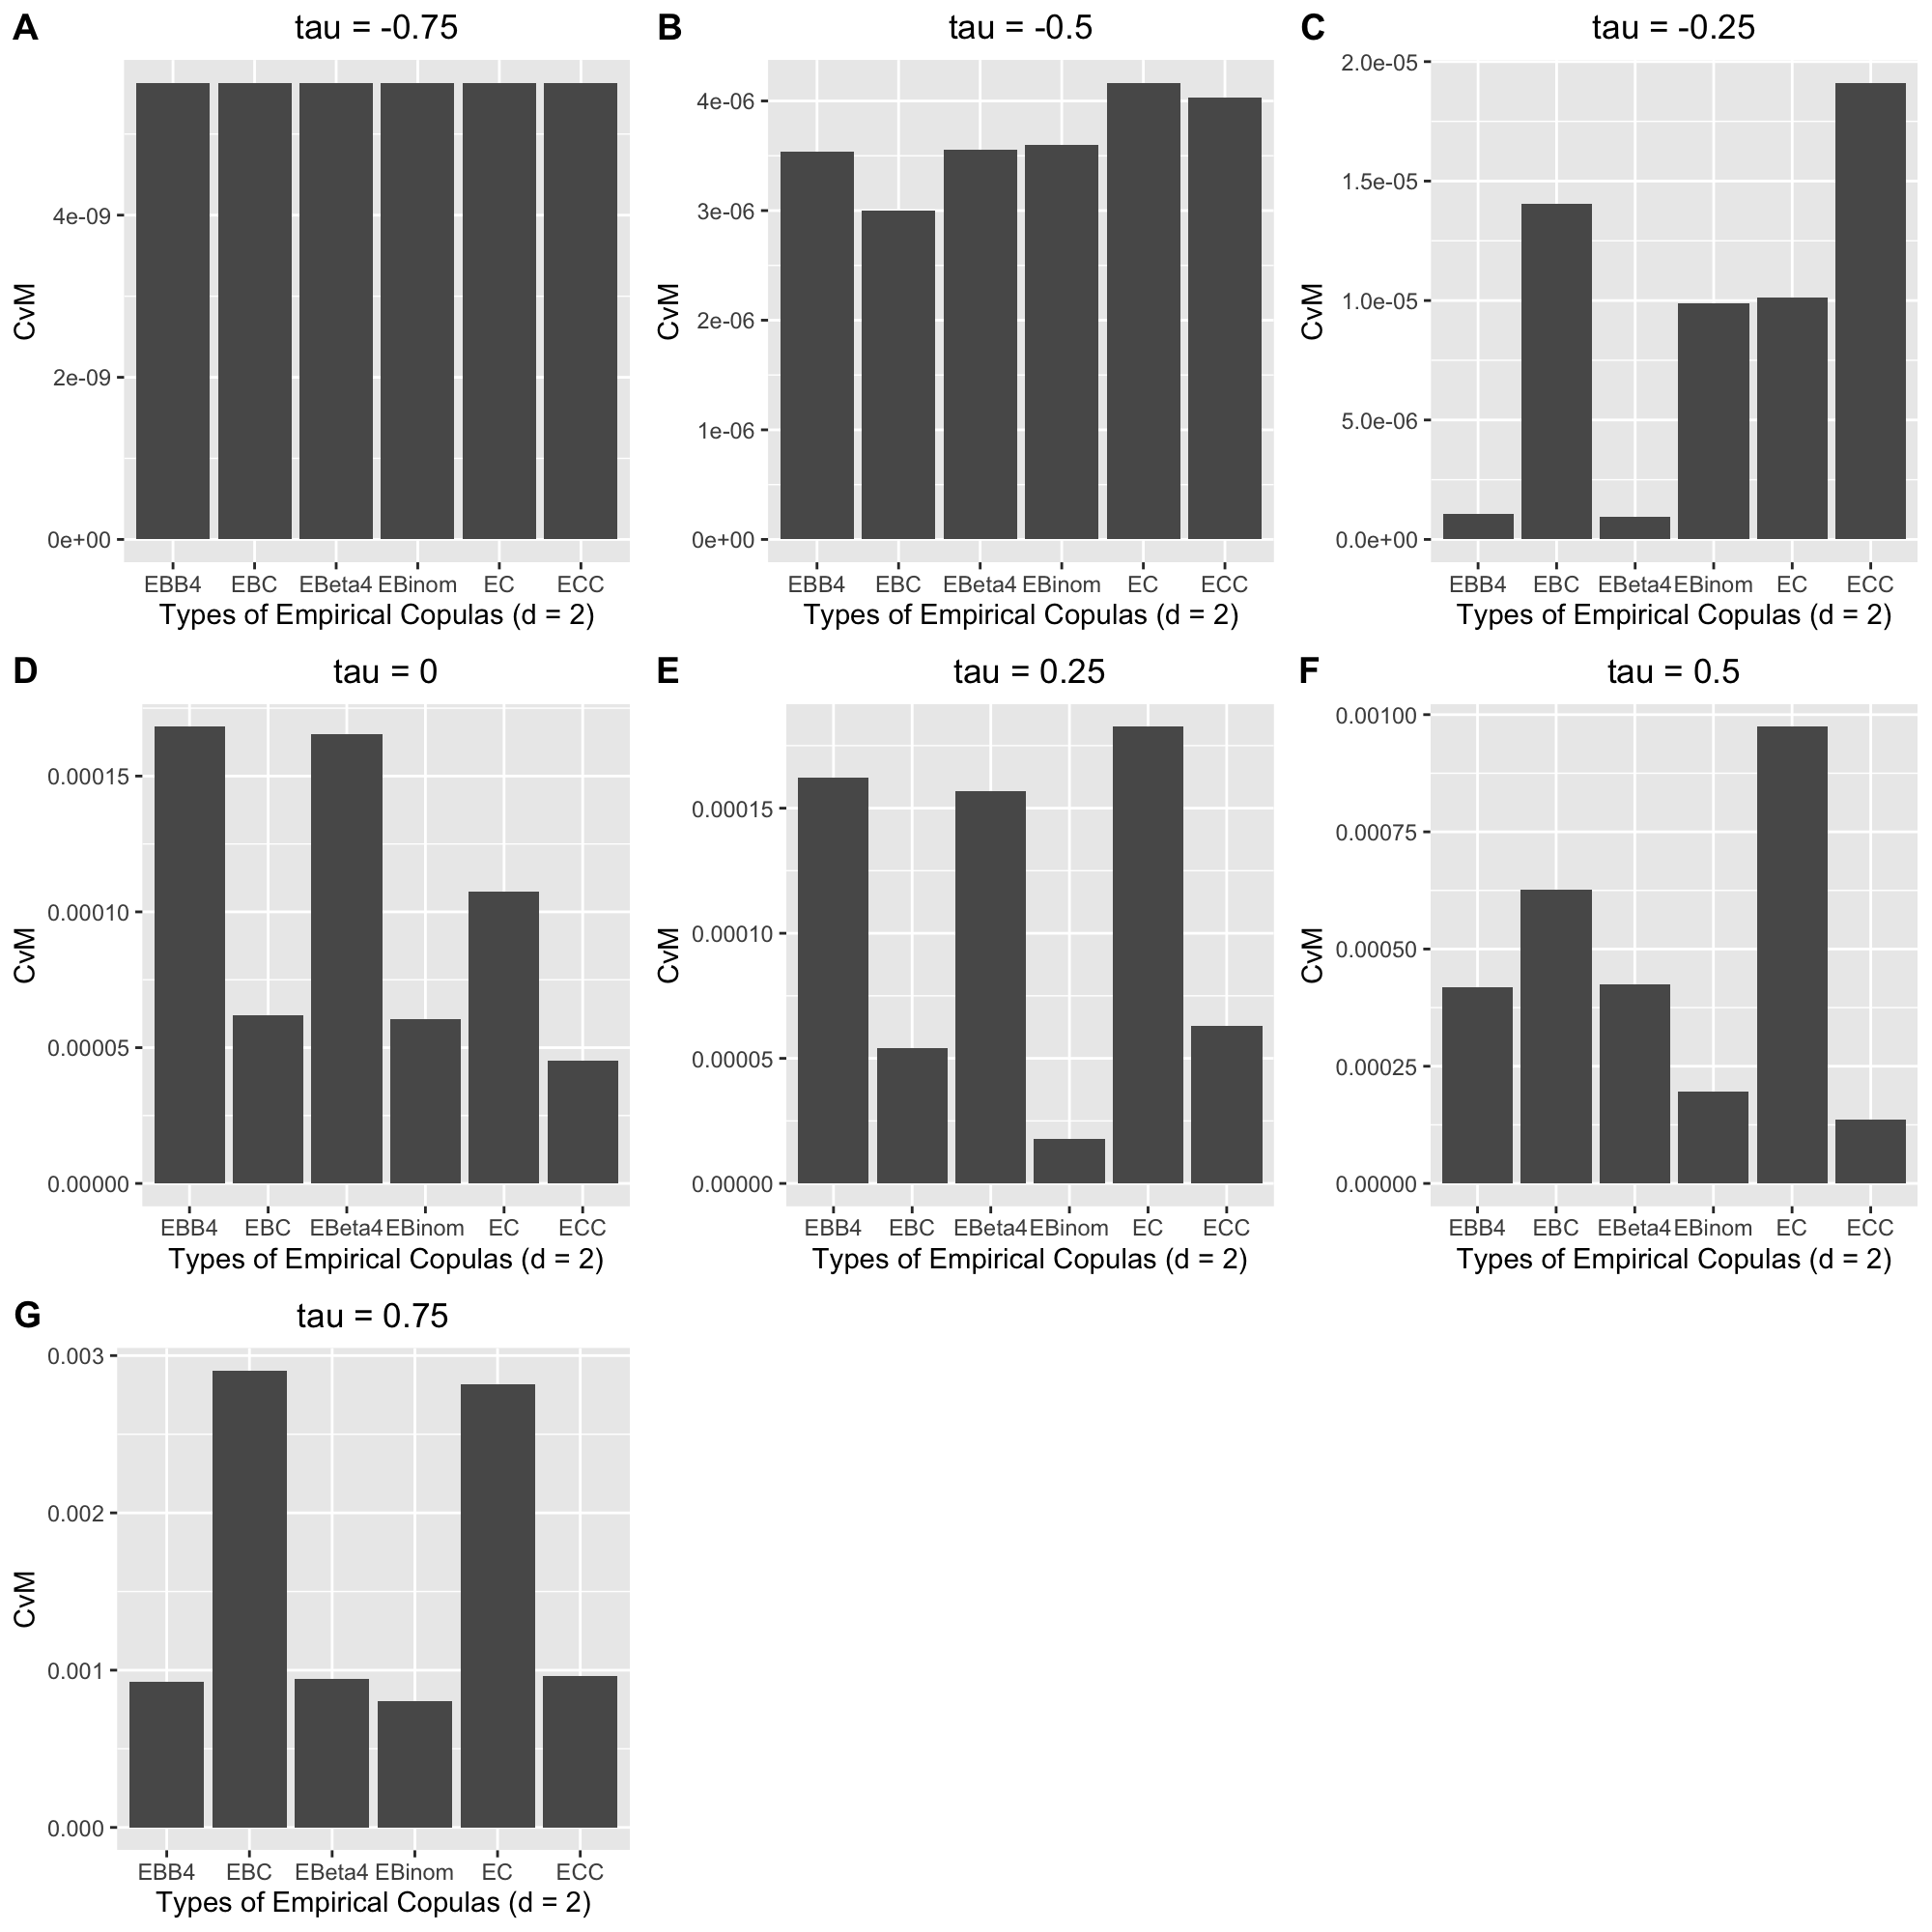
\includegraphics[width=17cm]{CumulativeCvM/t4_2d_c_CvM.png}
\captionof{figure}{Student-t copula with d = 2}
\end{center}%

\begin{center}
\label{N_2d_c_CvM}
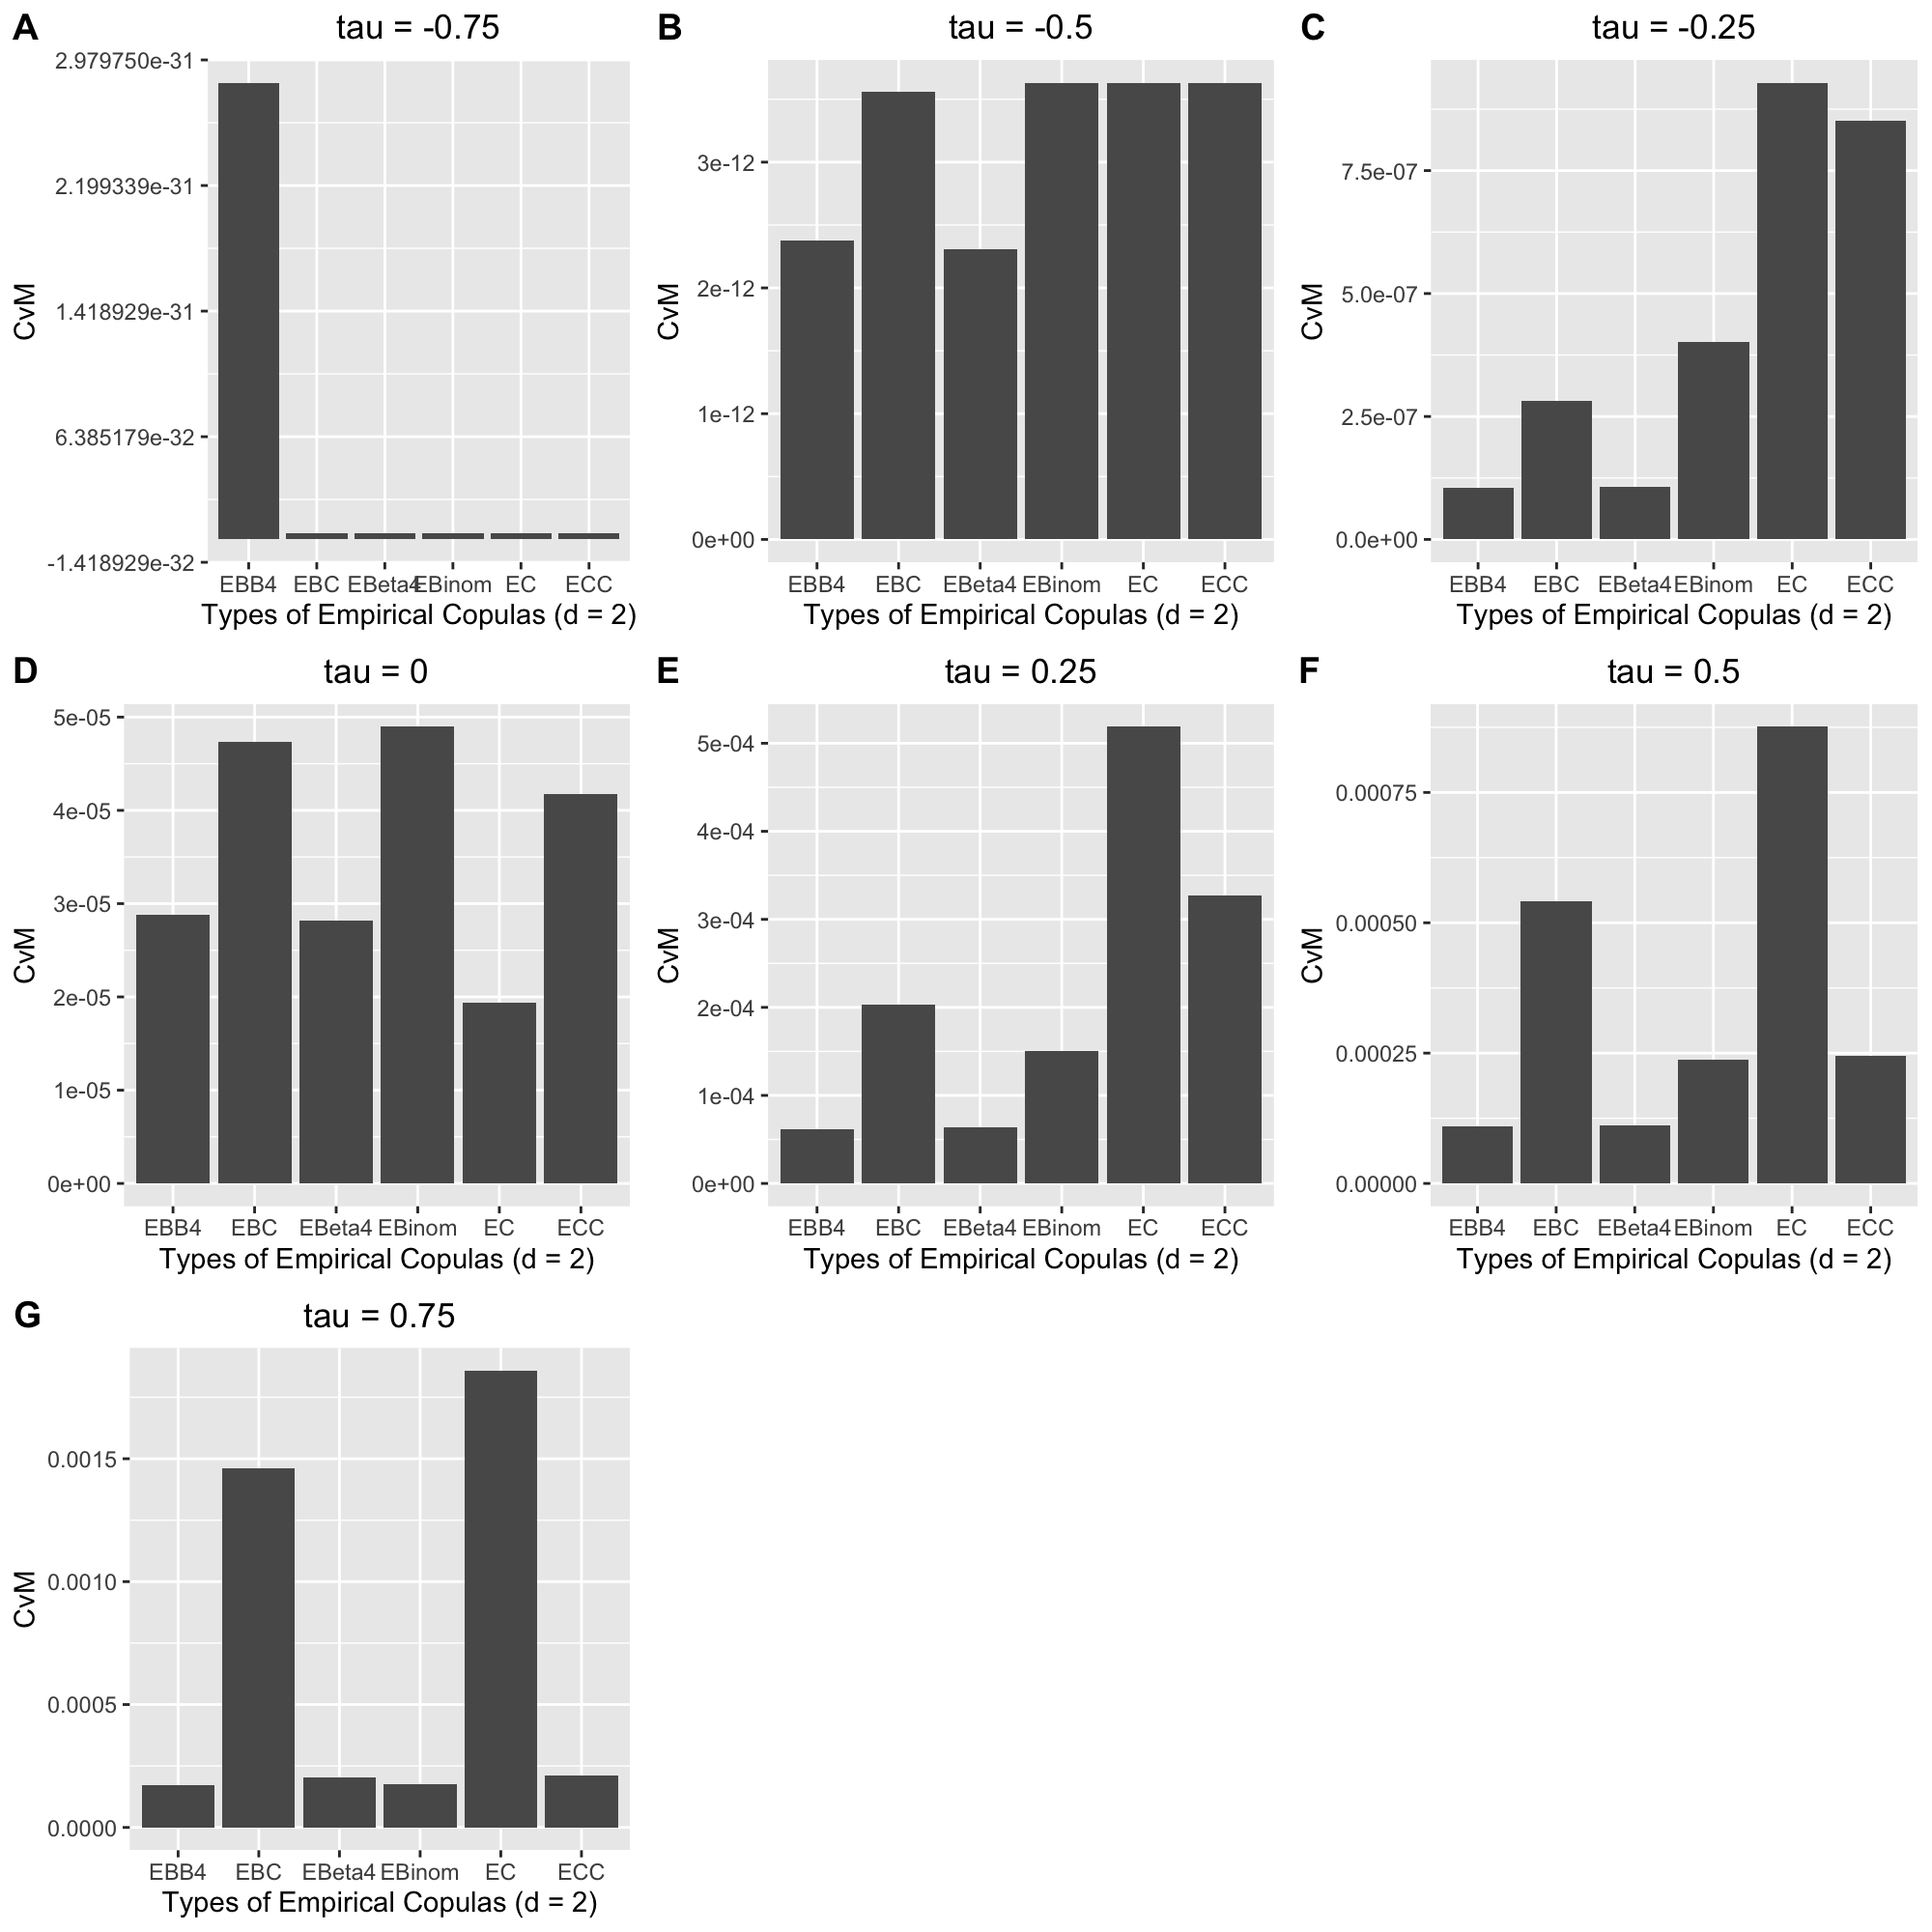
\includegraphics[width=17cm]{CumulativeCvM/N_2d_c_CvM.png}
\captionof{figure}{Gaussian copula with d = 2}
\end{center}%

\begin{center}
\label{C_2d_c_CvM}
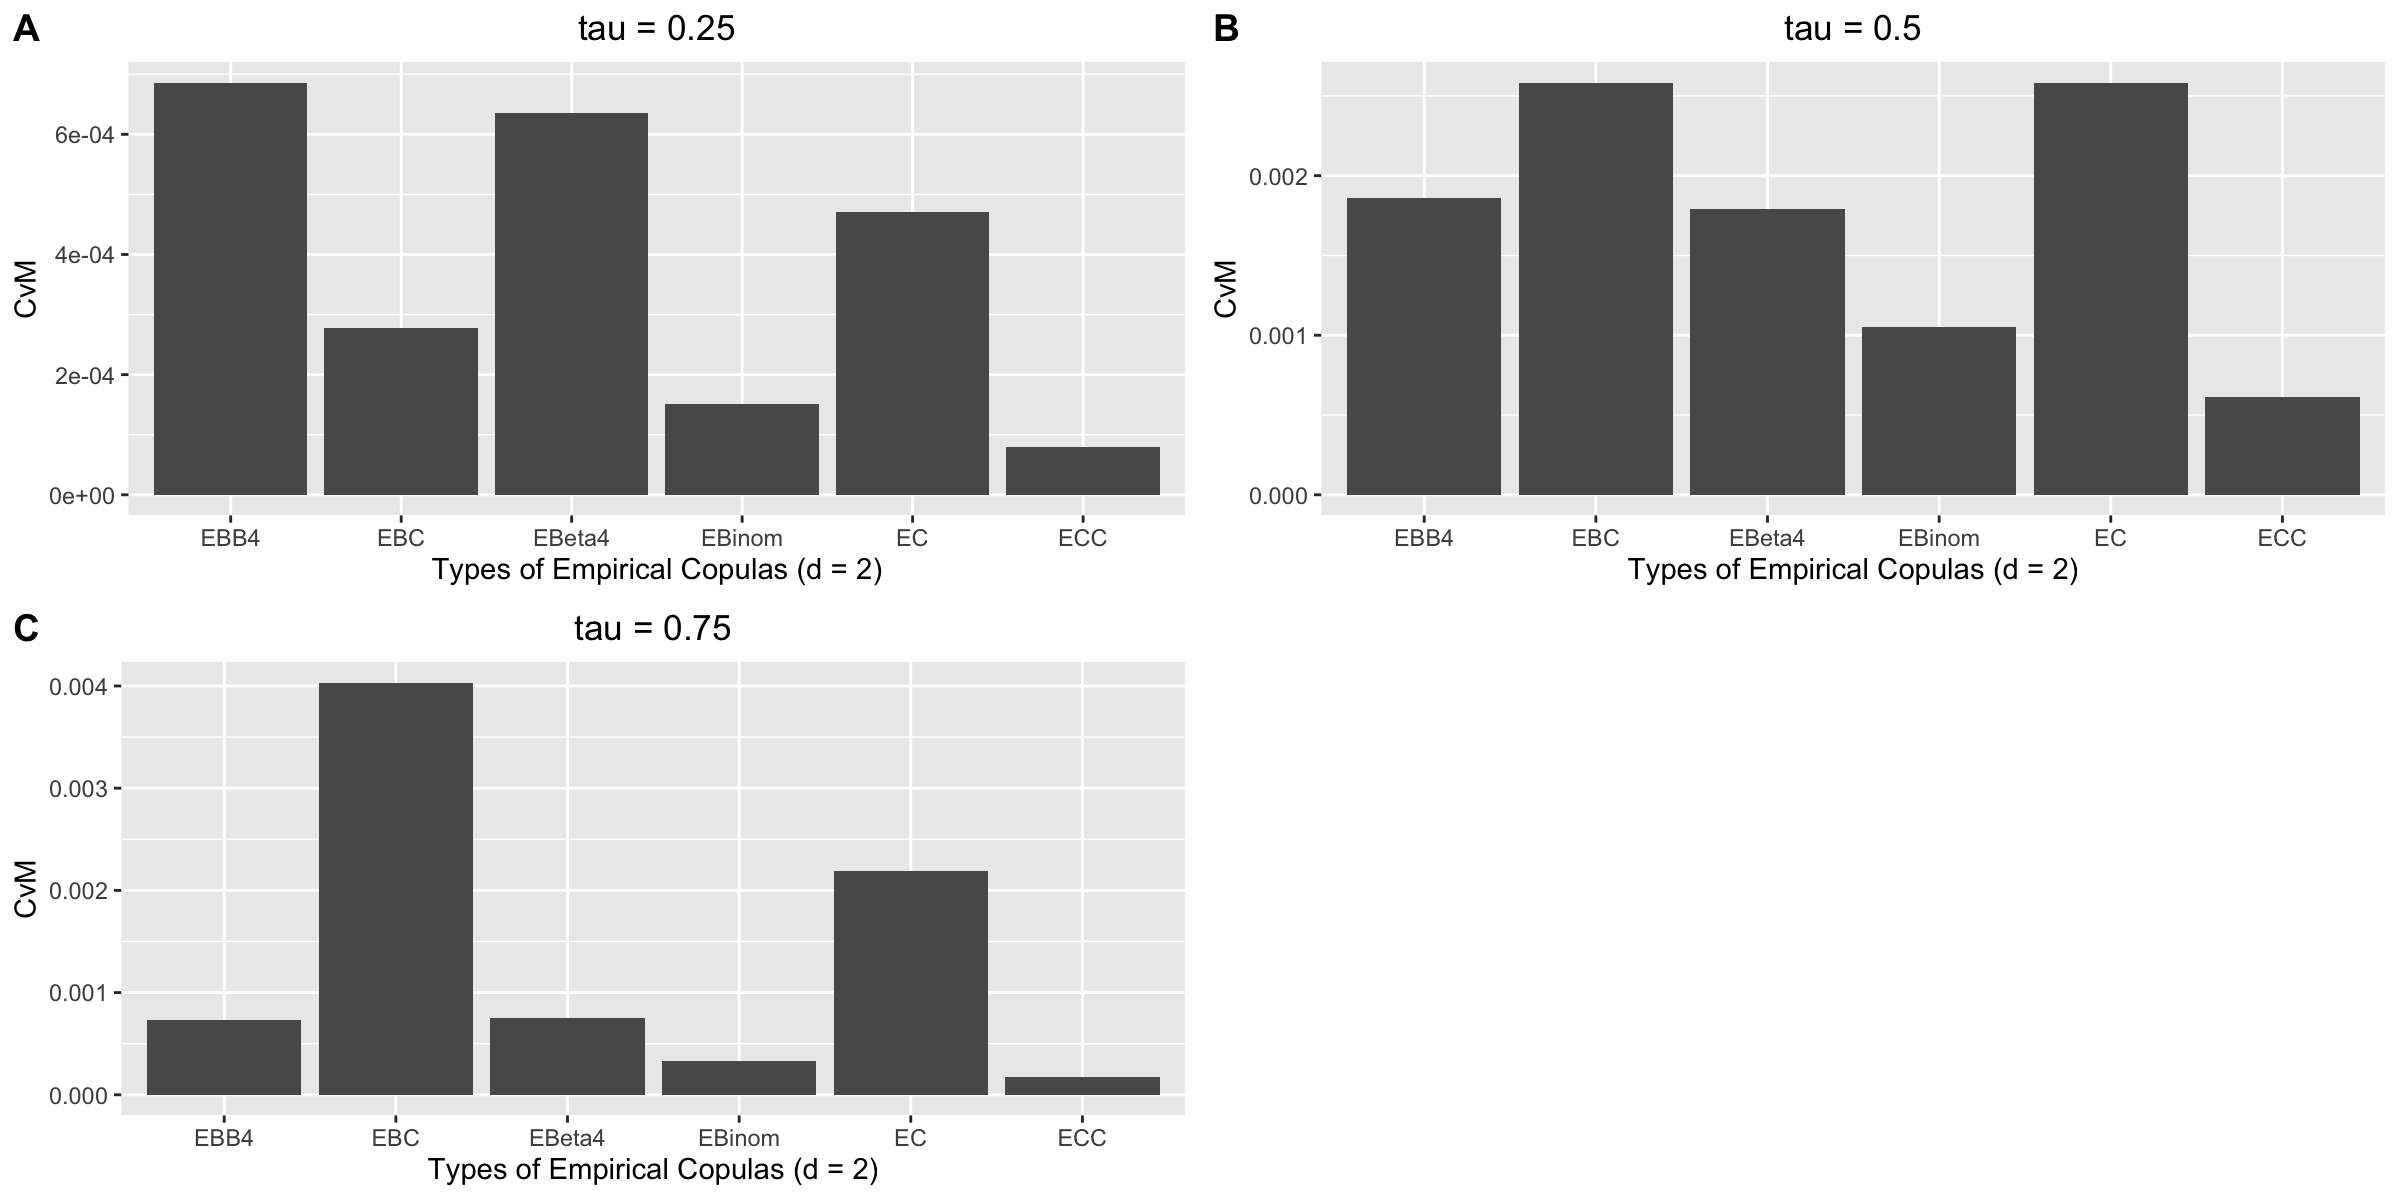
\includegraphics[width=17cm]{CumulativeCvM/C_2d_c_CvM.png}
\captionof{figure}{Clayton copula with d = 2}
\end{center}%

\begin{center}
\label{C_3d_c_CvM}
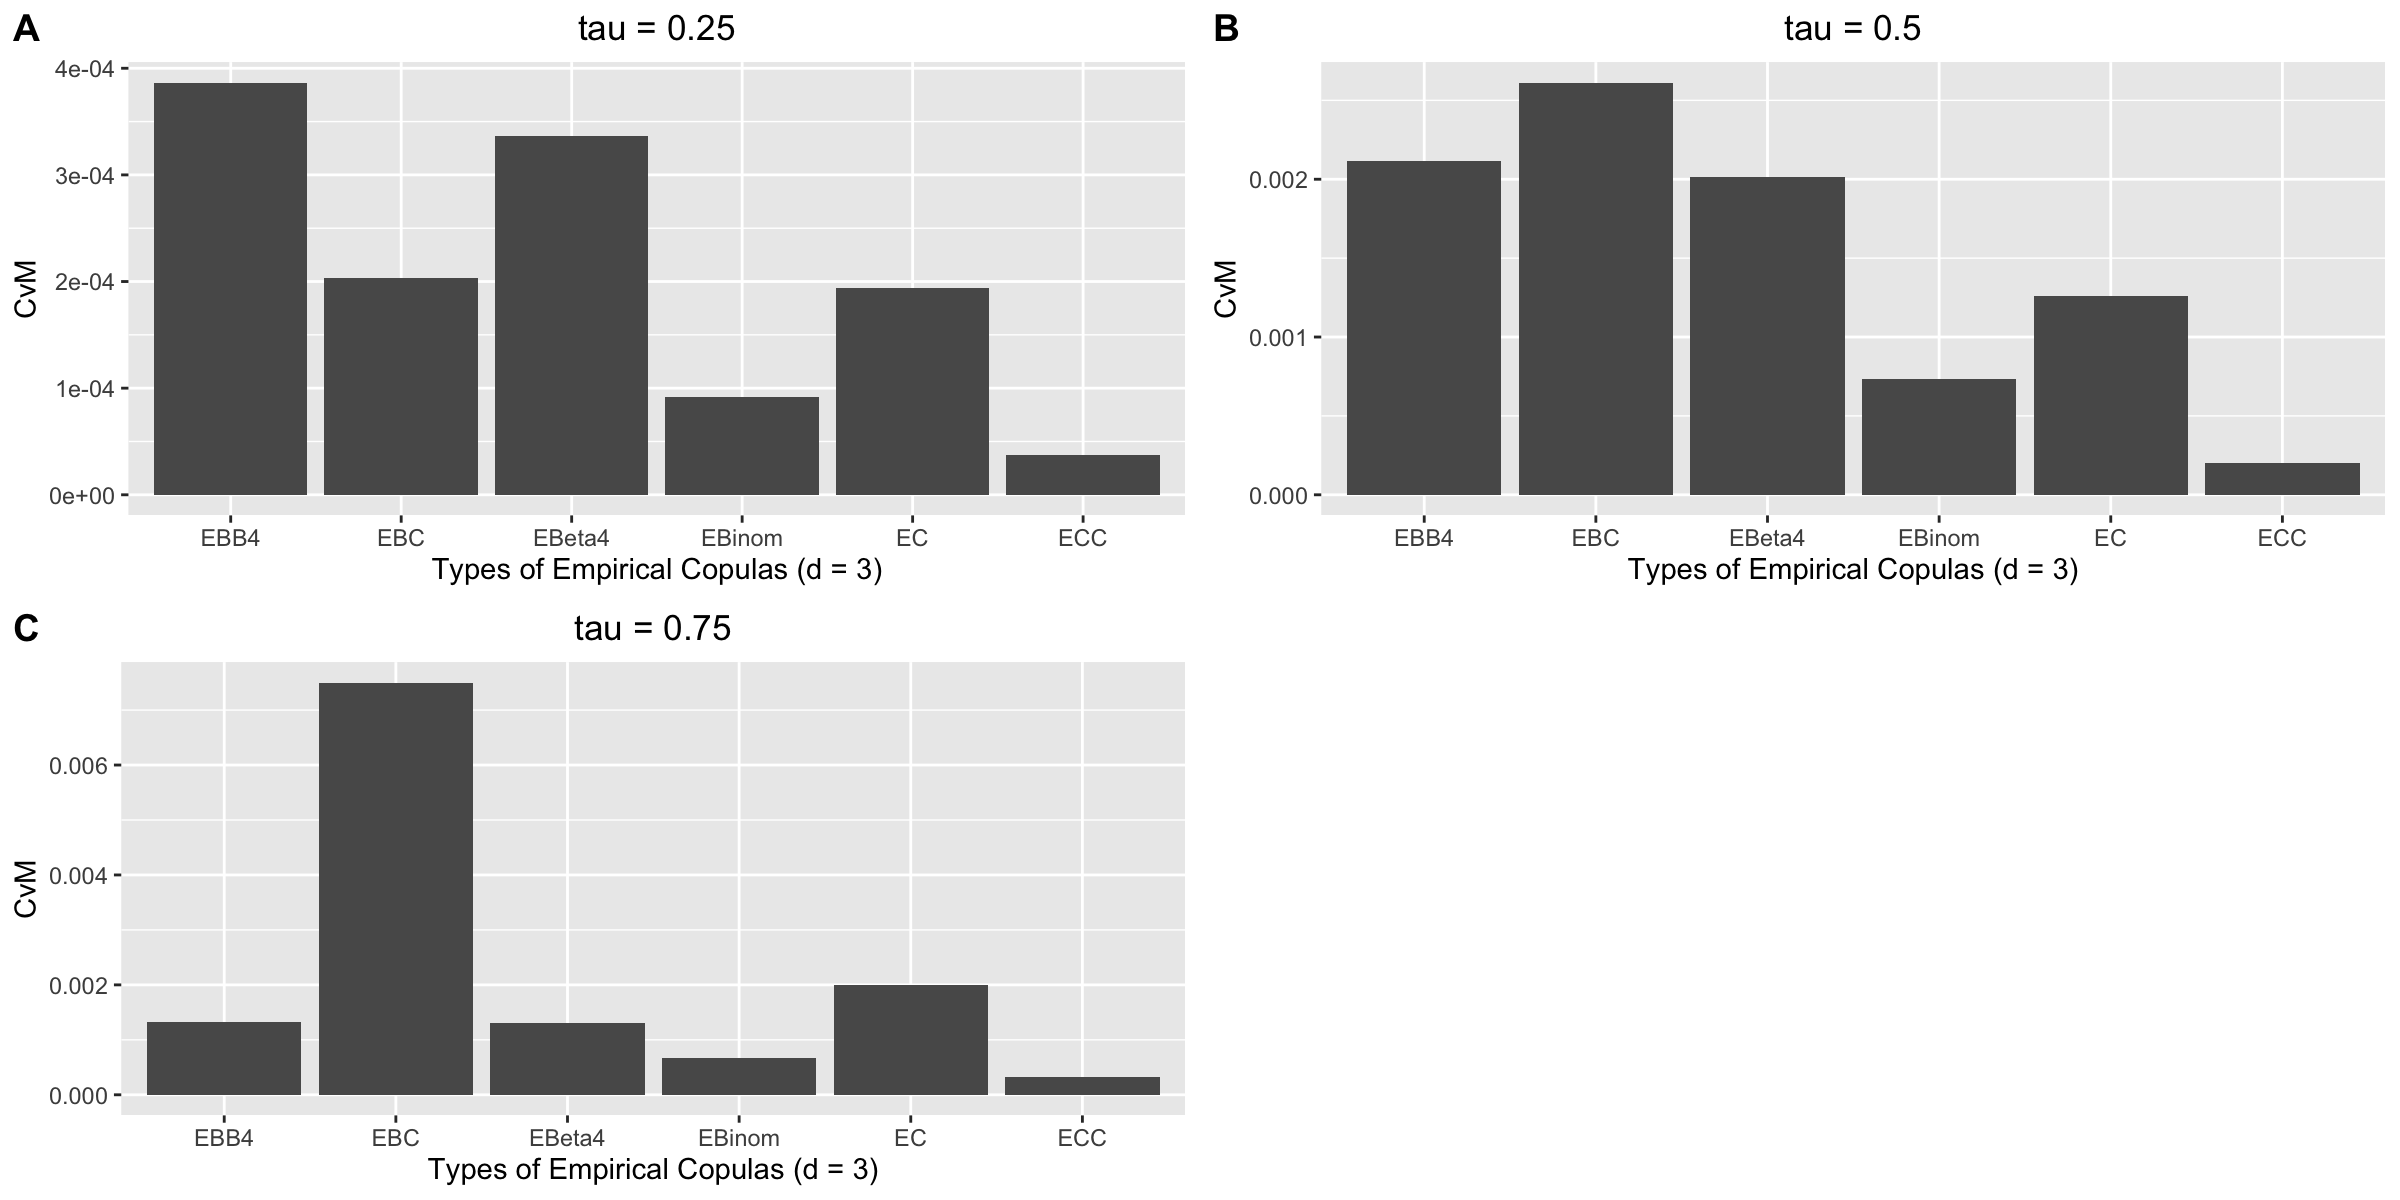
\includegraphics[width=17cm]{CumulativeCvM/C_3d_c_CvM.png}
\captionof{figure}{Clayton copula with d = 3}
\end{center}%

\begin{center}
\label{C_4d_c_CvM}
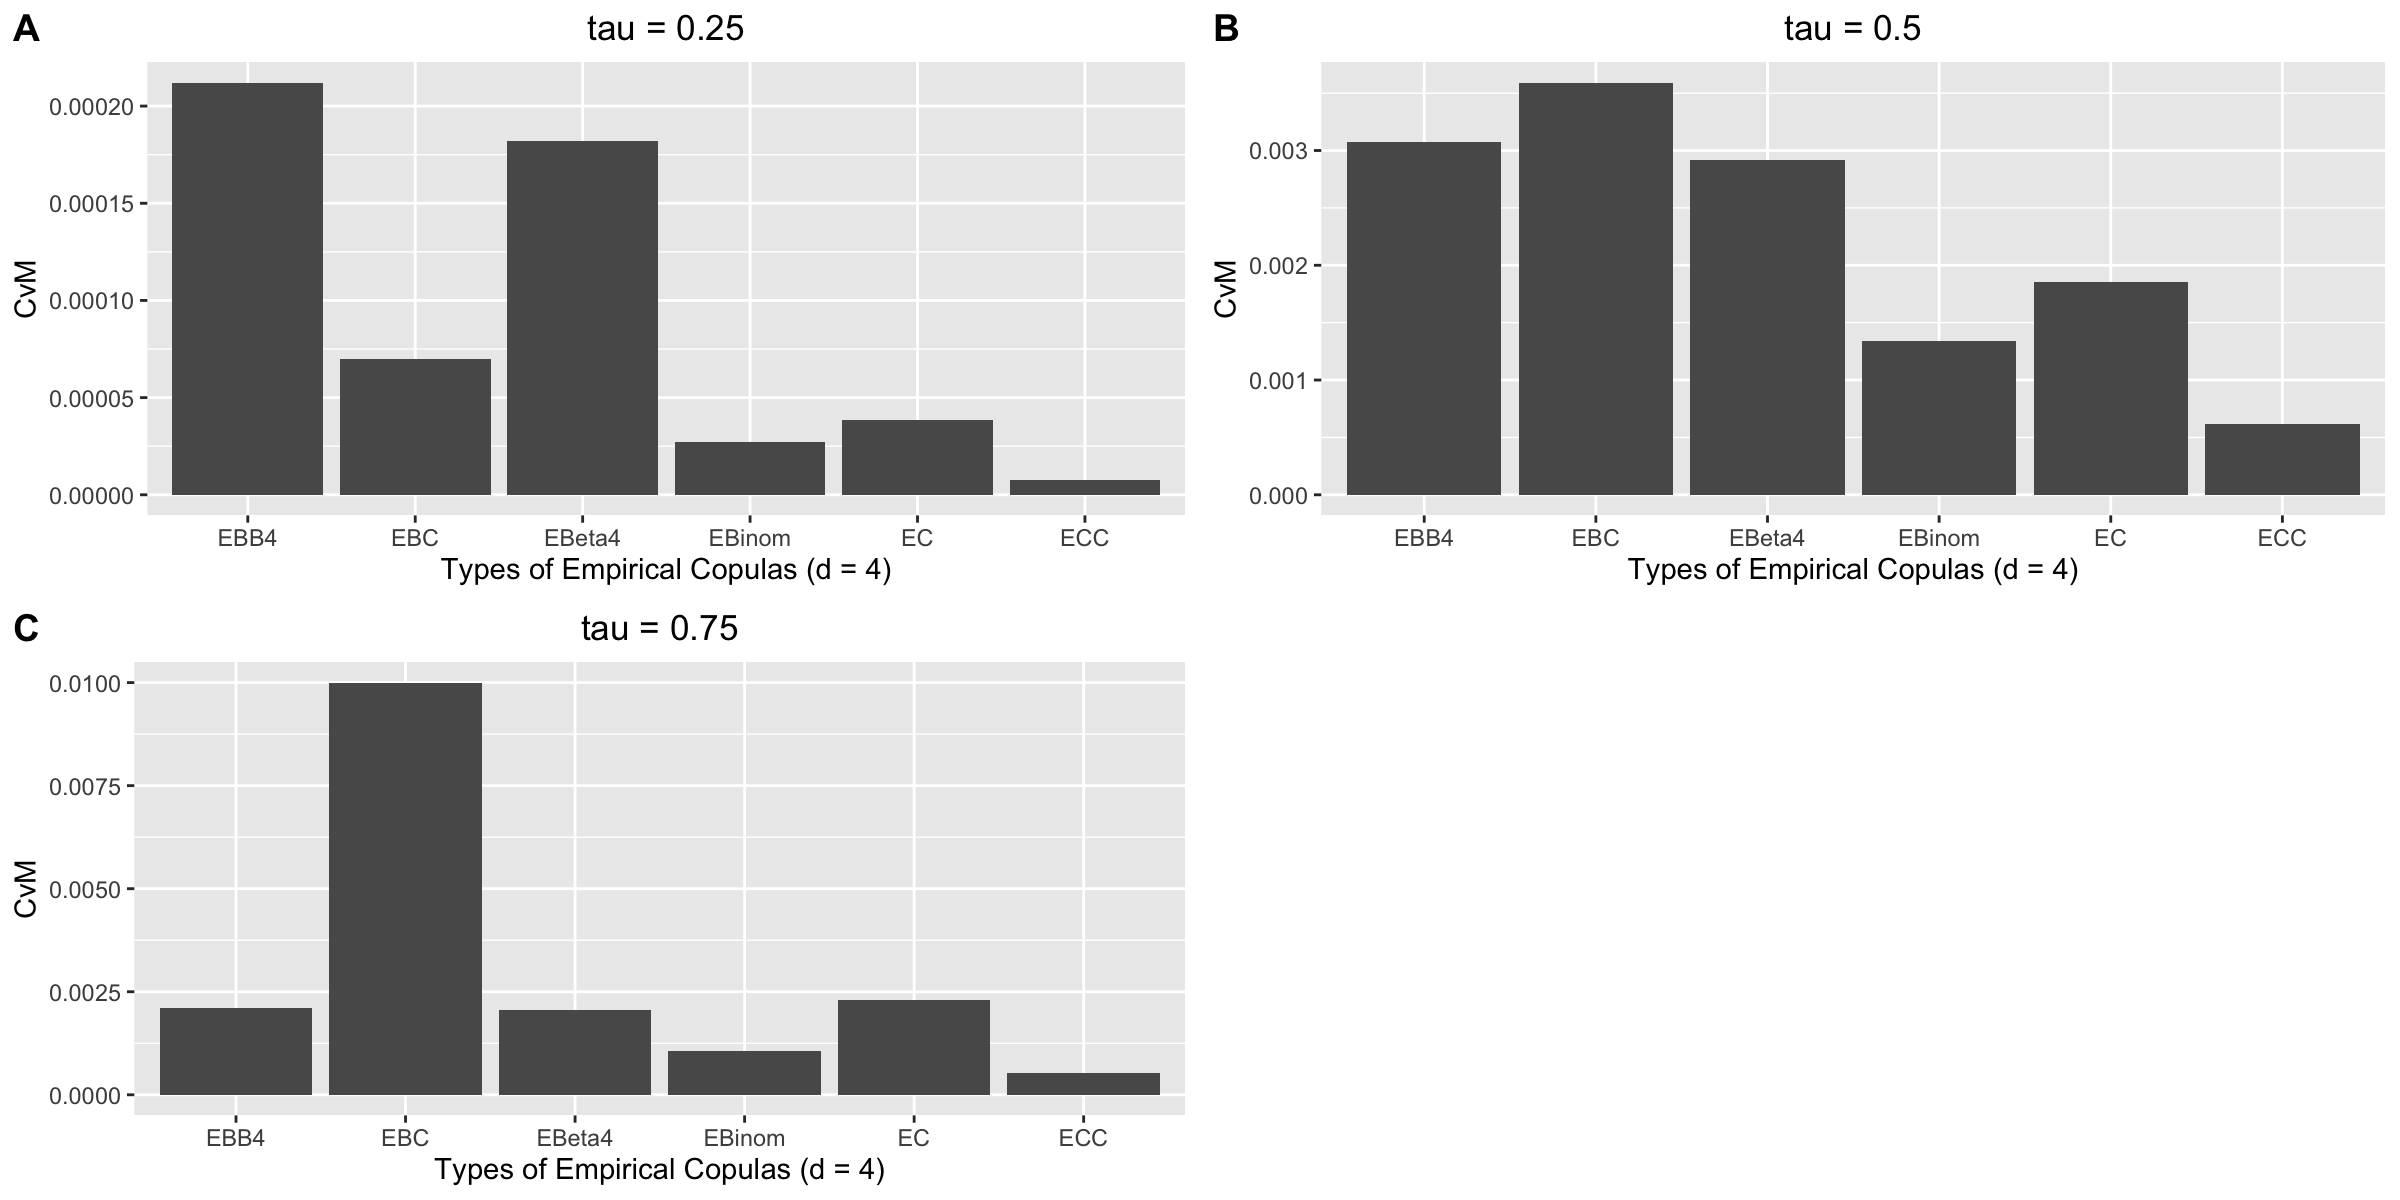
\includegraphics[width=17cm]{CumulativeCvM/C_4d_c_CvM.png}
\captionof{figure}{Clayton copula with d = 4}
\end{center}%

\begin{center}
\label{C_5d_c_CvM}
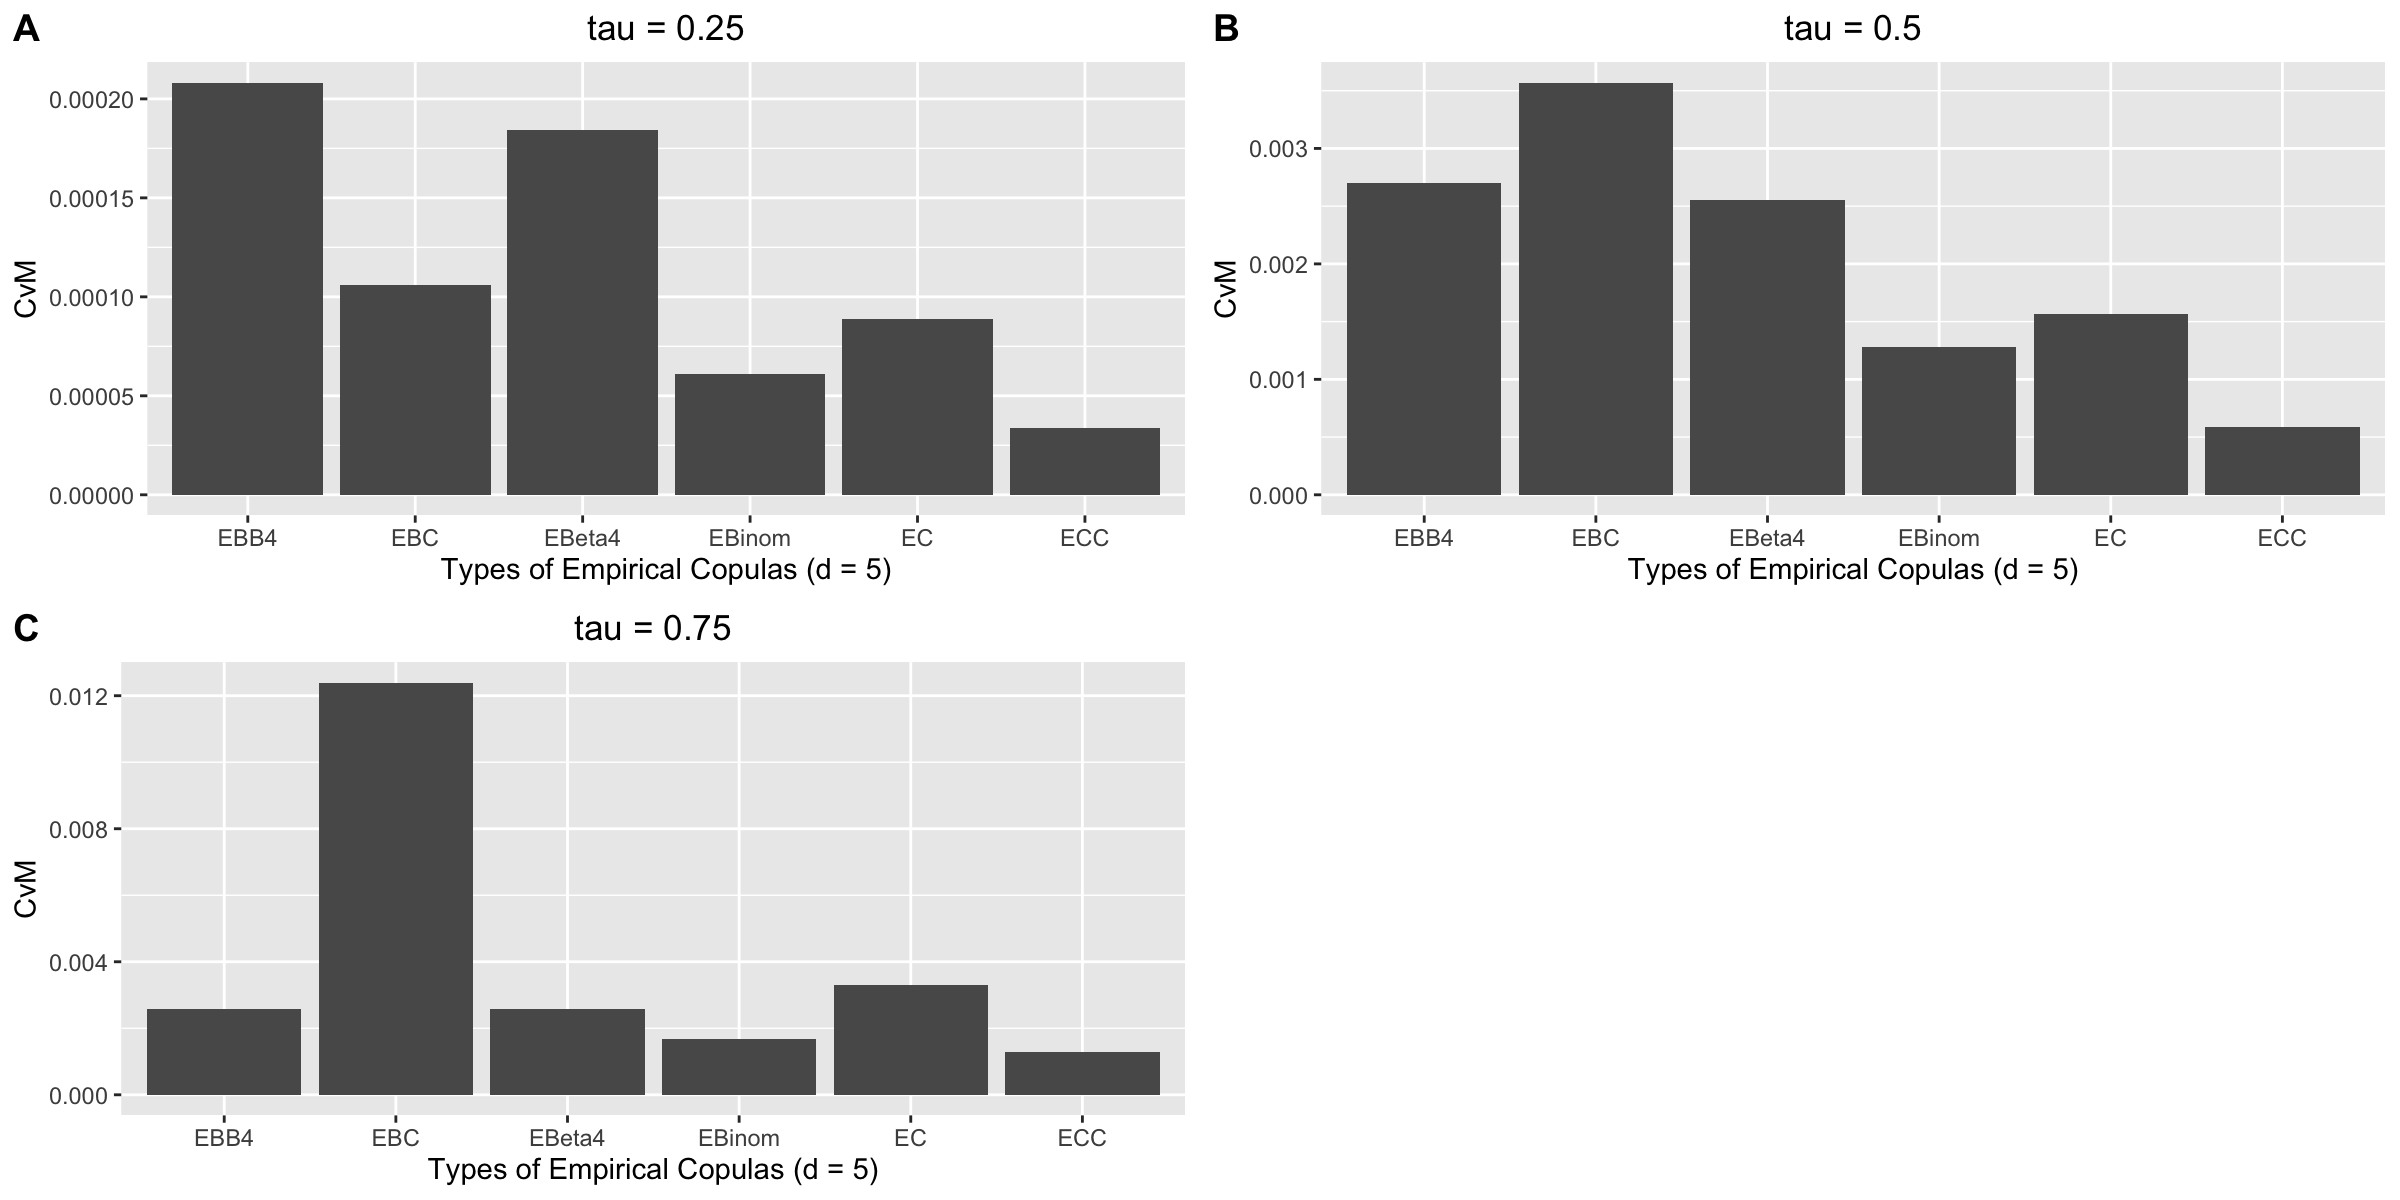
\includegraphics[width=17cm]{CumulativeCvM/C_5d_c_CvM.png}
\captionof{figure}{Clayton copula with d = 5}
\end{center}%

\newpage
\subsection{Analysis: Cumulative probabilities}


%3:3 -> 1000,1000$
%2:2 -> 1200,600$
\end{flushleft}
 
\medskip

\printbibliography
\end{document}
